%% ============================================================
%%  Master Thesis – Causal Shapley Values
%%  Juan David Rios Garcia
%%  LaTeX version – compile with: pdflatex -> bibtex -> pdflatex x2
%% ============================================================
\documentclass[12pt,a4paper,oneside]{article}

%% ── Encoding & fonts ────────────────────────────────────────
\usepackage[T1]{fontenc}
\usepackage[utf8]{inputenc}
\usepackage{lmodern}
\usepackage{microtype}

%% ── Page geometry ───────────────────────────────────────────
\usepackage[top=2.5cm, bottom=2.5cm, left=3cm, right=2.5cm, headheight=15pt]{geometry}

%% ── Line spacing ────────────────────────────────────────────
\usepackage{setspace}
\onehalfspacing

%% ── Mathematics ─────────────────────────────────────────────
\usepackage{amsmath}
\usepackage{amssymb}
\usepackage{mathtools}
\usepackage{bm}

%% ── Algorithms ──────────────────────────────────────────────
\usepackage{algorithm}
\usepackage{algpseudocode}
\algnewcommand\algorithmicinput{\textbf{INPUT:}}
\algnewcommand\INPUT{\item[\algorithmicinput]}
\algnewcommand\algorithmicoutput{\textbf{OUTPUT:}}
\algnewcommand\OUTPUT{\item[\algorithmicoutput]}
\algnewcommand\algorithmicprecompute{\textbf{PRECOMPUTE:}}
\algnewcommand\PRECOMPUTE{\item[\algorithmicprecompute]}

%% ── Tables ──────────────────────────────────────────────────
\usepackage{booktabs}
\usepackage{tabularx}
\usepackage{multirow}
\usepackage{array}
\newcolumntype{L}[1]{>{\raggedright\arraybackslash}p{#1}}
\newcolumntype{C}[1]{>{\centering\arraybackslash}p{#1}}
\newcolumntype{R}[1]{>{\raggedleft\arraybackslash}p{#1}}

%% ── Graphics & figures ──────────────────────────────────────
\usepackage{graphicx}
\usepackage{float}
\usepackage{subcaption}
\usepackage{caption}
\captionsetup{font=small, labelfont=bf, margin=1cm}

%% ── Colours ─────────────────────────────────────────────────
\usepackage[dvipsnames,table]{xcolor}
\definecolor{algblue}{HTML}{2c4a6e}
\definecolor{algbg}{HTML}{eef2f7}

%% ── Hyperlinks ──────────────────────────────────────────────
\usepackage[hidelinks, breaklinks=true,
            pdfauthor={Juan David Rios Garcia},
            pdftitle={Evaluating the Impact of Discovered Causal Structures on
                      Structure-Aware Shapley Methods}]{hyperref}

%% ── References ──────────────────────────────────────────────
\usepackage[numbers,sort&compress]{natbib}
\bibliographystyle{plainnat}

%% ── Miscellaneous ───────────────────────────────────────────
\usepackage{enumitem}
\usepackage{parskip}
\setlength{\parskip}{6pt}
\usepackage{fancyhdr}
\pagestyle{fancy}
\fancyhf{}
\fancyhead[R]{\small\nouppercase{\leftmark}}
\fancyfoot[C]{\thepage}
\renewcommand{\headrulewidth}{0.4pt}

%% ── Custom algorithm box style ──────────────────────────────
\makeatletter
\renewcommand{\ALG@name}{Algorithm}
\makeatother

%% ============================================================
\begin{document}
%% ============================================================

%% ── Title page ──────────────────────────────────────────────
\begin{titlepage}
  \centering
  \vspace*{2cm}
  {\LARGE\bfseries Evaluating the Impact of Discovered Causal Structures on\\[0.4em]
  Structure-Aware Shapley Methods:\\[0.4em]
  An Experimental Pipeline\par}
  \vspace{2cm}
  {\large Juan David Rios Garcia\par}
  \vfill
  {\large Master Thesis\par}
  \vspace{1cm}
  {\large 2026\par}
\end{titlepage}

\newpage
\tableofcontents
\newpage

%% ============================================================
\section{Introduction}
\label{sec:intro}
%% ============================================================

Model explainability has become a fundamental prerequisite for the deployment of machine learning systems, particularly across high-stakes socioeconomic domains such as credit scoring, healthcare access, and public resource allocation, where algorithmic decisions must be transparently justified to affected individuals and regulatory bodies \citep{Baron2023}.

While Shapley values derived from cooperative game theory have emerged as a gold standard for local feature attribution due to their unique axiomatic foundations, traditional implementations frequently rely on the simplifying assumption of feature independence. This assumption treats all feature permutations as equally probable during coalition formation, which can systematically misattribute credit when the true generative process involves structured causal dependencies among inputs \citep{Lundberg2017, Heskes2020}.

To mitigate these limitations, recent literature has introduced structure-aware Shapley frameworks that explicitly embed topological and causal constraints into the attribution process. Asymmetric Shapley Values (ASV) restrict permutations to those consistent with a causal ordering \citep{Frye2021}; Causal Shapley Values (CSV) replace observational marginalization with interventional conditioning based on Pearl's do-calculus \citep{Heskes2020}; and Shapley Flow reframes credit assignment from nodes to directed edges in a causal graph \citep{Wang2021}. Each of these methods promises attributions that are more faithful to the underlying causal mechanism that generated the data.

Historically, these structure-aware Shapley frameworks have been demonstrated almost exclusively on well-characterized systems, domains backed by years of research where the causal links between variables are firmly established and treated as ground truth. A different situation arises far more often in practice: a practitioner suspects that causal relationships exist among the features of a system but cannot point to a validated graph describing them. In this setting, a traditional Shapley computation will ignore those dependencies entirely, distributing credit as if every feature were an independent, interchangeable coalition partner. The practitioner is therefore caught between a method that disregards causal structure and a family of methods that assume it is already known.

A critical bottleneck in prior work is the assumption that the underlying Causal Directed Acyclic Graph (DAG) is known \emph{a priori} or completely specified by a domain expert. In practical applications, the true causal graph is almost never directly observable. Practitioners must instead rely on automated causal discovery algorithms such as the constraint-based PC algorithm \citep{Spirtes2000} and the functional causal model DirectLiNGAM \citep{Shimizu2011} to infer a plausible graph structure from observational data. These estimated graphs are inherently noisy, subject to false-positive and false-negative edge errors, and sensitive to violations of their underlying assumptions \citep{Glymour2019}.

This thesis addresses this open gap by constructing a comprehensive experimental pipeline that integrates automated causal discovery directly into structure-aware explainability frameworks and systematically measures how graph estimation errors propagate downstream into feature attribution outputs. The pipeline evaluates three structure-aware Shapley methods (Asymmetric Shapley, Causal Shapley, and Shapley Flow) under three causal graph sources: the PC-discovered graph, the LiNGAM-discovered graph, and the True DAG used as an oracle reference. Evaluation is performed on two benchmarks: a controlled synthetic dataset with 50 features and known linear causal structure, and the real-world Sachs cell signaling dataset \citep{Sachs2005}, where an established consensus DAG allows external validation.

The central research question is: when a practitioner feeds an imperfect discovered causal graph into a structure-aware Shapley method, does the method produce attributions that meaningfully differ from a graph-free baseline, and do those attributions move closer to or further from the oracle attributions obtained with the True DAG? The answer has direct implications for how causal explainability tools should be adopted in practice.

To answer this question consistently, the analysis tracks two dimensions along which an attribution can shift when causal structure is injected: the \emph{magnitude} of the attribution assigned to a feature and the \emph{direction} (sign) of that attribution. This separation is deliberate. Prior comparisons of attribution methods overwhelmingly report how much the size of the attributions changes, while the question of whether a feature's contribution flips from pushing a prediction up to pushing it down is reported far less often, even though a sign reversal is arguably the more consequential failure for a practitioner trying to explain a single decision. A graph that merely rescales attributions still preserves the qualitative story told to an affected individual; a graph that inverts signs tells the opposite story. Both dimensions therefore matter, and they can move independently: a method may keep magnitudes stable while reordering signs, or preserve signs while inflating magnitudes. The two dimensions are operationalized by a single metric each, used identically across every comparison: a Magnitude Divergence and a Sign Disagreement, each reported relative to a named reference (the graph-free baseline, the oracle DAG, or the opposite discovered graph). The mathematical logic of both metrics are detailed deeply in Section~\ref{sec:metrics}. Thanks to this dual-axis approach operating independently of any specific dataset or model architecture, it establishes a universal, replicable framework for future work; for now, setting magnitude and direction as our primary analytical axes provides the definitive standard needed to assess the viability of any structure-aware method in real-world scenarios.

%% ============================================================
\section{Conceptual Framework and Methodology}
\label{sec:framework}
%% ============================================================

\subsection{Model Explainability and Causal Understanding}

A fundamental distinction must be established regarding the objective of model explainability. Rather than attempting to reveal the underlying laws of a real-world physical system, the focus of this work is strictly bounded to explaining the predictive behavior of a trained machine learning model. This distinction mirrors the conceptual separation established by \citet{Baron2023} between causal understanding of nature and causal understanding of a model's decision function.

In practical machine learning scenarios, conducting physical manipulations or randomized controlled treatments is often expensive, time-consuming, or ethically impossible. Consequently, model explanations must be grounded in the observational data distribution used during training, while ideally respecting the causal relationships that govern how features jointly determine model outputs. Structure-aware Shapley methods operationalize this grounding by encoding causal relationships as constraints on the attribution computation, rather than by performing physical interventions.

\subsection{Counterfactual Explanations and the Structural Causal Model Framework}

Counterfactual explanations provide an intuitive contrastive explainability framework by identifying the minimal input feature perturbations required to alter an algorithmic output \citep{Wachter2018}. Standard optimization methods, however, generate counterfactuals that may violate physical plausibility constraints by placing instances in low-density regions of the joint feature space or proposing changes that contradict causal relationships \citep{Mahajan2020}.

To satisfy real-world feasibility constraints, explanations must be grounded within a Structural Causal Model (SCM), formally defined as a tuple $\mathcal{G} := (\mathcal{S}, P(\varepsilon))$, where $\mathcal{S}$ is a collection of deterministic structural equations of the form $x_i = f_i(\mathrm{Pa}(x_i), \varepsilon_i)$, and $P(\varepsilon)$ is a joint distribution over independent exogenous noise variables \citep{Pearl2009}. Full abduction-action-prediction within an SCM is computationally demanding and requires complete structural equation knowledge. Structure-aware Shapley methods circumvent this bottleneck by using the causal graph topology to define conditional distributions for feature imputation, approximating the post-interventional distribution without requiring full structural equation reconstruction.

It is worth noting that the original Shapley Flow formulation \citep{Wang2021} relies heavily on approximating these structural equations to actively propagate values along graph edges. However, for reproducibility purposes and to avoid strict dependence on a well-calibrated SCM, the implementation adopted in this thesis deliberately replaces full structural-equation evaluation with a lighter binary activation rule (detailed in Section~\ref{sec:flow}). This approach preserves the framework's core conceptual contribution, attributing credit to directed edges rather than isolated nodes, while ensuring tractable computation that relies solely on the discovered graph topology and trained predictive model.

\subsection{Causal Discovery: Structure Identification}

Estimating the causal graph is a critical step in the experimental pipeline. Two prominent causal discovery algorithms are utilized:

\paragraph{PC Algorithm \citep{Spirtes2000}.} A constraint-based method that recovers the causal skeleton through conditional independence tests (Fisher-z at $\alpha = 0.05$) and applies Meek's orientation rules to produce a Completed Partially Directed Acyclic Graph. Undirected edges are resolved by orienting them from lower to higher feature index, yielding a valid DAG for downstream Shapley computation.

\paragraph{DirectLiNGAM \citep{Shimizu2011}.} A functional causal model that exploits linear non-Gaussian structures to simultaneously identify causal ordering and structural coefficients. Each entry in the estimated adjacency matrix represents the linear weight a parent contributes to a child. Because DirectLiNGAM initially returns a dense matrix containing minor estimation noise, a magnitude threshold is applied to recover a sparse structure. Edges with an absolute coefficient below $0.10$ are pruned; this cutoff effectively treats weak direct effects as noise, maintaining a graph density comparable to the other configurations without discarding meaningful dependencies.

Both algorithms operate strictly on the $X$-only training partition, excluding the target for the discovery step. While both the synthetic dataset and the real-world biological data likely do not perfectly fulfill all the theoretical requirements of these algorithms, this imperfection is deliberate. It serves as a realistic robustness test, reflecting the natural unmeasured confounding and structural uncertainty practitioners face in deployment.

\subsection{Traditional Shapley Values and the Axiomatic Framework}

Traditional Shapley values originate in cooperative game theory as the unique solution to the problem of fairly dividing the total payoff of a game among the players who produced it \citep{Shapley1953}. In the explainability transfer of this idea, the players are the input features, the coalition is any subset $S$ of features whose values are known, and the payoff of a coalition is the model output produced when only those features take their actual instance values while the remaining features are treated as absent. A feature that is in the coalition contributes its real value $x_j$; a feature that is out of the coalition is marginalized over the background distribution, so the model is evaluated as if that feature's value were unknown and drawn from the data at large. The marginal contribution of a feature is then the change in the payoff caused by moving that feature from outside the coalition to inside it, that is, the difference $f(S \cup \{i\}) - f(S)$ between the model output with the feature added and the model output without it.

Because this marginal contribution depends on which features are already present, the Shapley value averages it over every order in which the features could be added to the coalition. Concretely, for a given permutation of the features each feature is added one at a time, its marginal contribution against the coalition of all features preceding it in that order is recorded, and the Shapley value of a feature is the average of these marginal contributions taken over all $N!$ permutations. Averaging over all orderings is precisely what makes the allocation fair in the game-theoretic sense and is what guarantees the four axioms below. The construction satisfies \textbf{Efficiency} (the attributions sum to the gap between the prediction for the instance and the average prediction, $f(x)$ minus the baseline), \textbf{Linearity} (attributions from model ensembles combine linearly), \textbf{Null Player} (zero attribution for features with no marginal contribution in any coalition), and \textbf{Symmetry} (two features that contribute identically to every coalition receive equal credit). The Symmetry axiom is too restrictive for causal systems: it treats all features as interchangeable coalition partners, weighting every ordering equally, which misattributes credit from downstream effects to upstream causes when the two are correlated through the causal structure.

\subsection{Structure-Aware Shapley Methods: Theoretical Foundations}

Structure-aware Shapley frameworks preserve Efficiency, Linearity, and Nullity while modifying or relaxing Symmetry to accommodate causal topologies.

\subsubsection{Asymmetric Shapley Values (ASV)}

ASV breaks the Symmetry axiom by replacing the uniform distribution over feature orderings with a weighting scheme $w(\pi)$ that places probability mass exclusively on permutations consistent with a partial causal ordering \citep{Frye2021}. Concretely, the causal DAG is used to derive a topological order over the features, and only those permutations that respect this order---in which every ancestor appears before each of its descendants---are admitted into the averaging. This restriction shrinks the permutation universe relative to Traditional Shapley: instead of averaging over all $N!$ orderings, ASV averages only over the valid linear extensions of the partial order encoded by the graph, a strict subset whose size shrinks as the graph becomes more connected. Ancestral causes therefore always precede their downstream effects during coalition formation, preventing descendant features from receiving credit for contributions mediated by their ancestors.

Apart from this restriction on the ordering, ASV is mechanically identical to Traditional Shapley. The notion of a coalition is unchanged, features inside the coalition take their instance values and features outside it are marginalized over the background distribution, and the marginal contribution is still the same difference $f(S \cup \{i\}) - f(S)$ evaluated through the model. ASV retains observational marginalization for absent features, constraining only the permutation space and not the imputation distribution; the DAG enters the computation solely through the set of admissible orderings.

Formally, the attribution is the expectation of a feature's marginal contribution taken over orderings drawn uniformly from the topological orderings of the feature DAG:
\begin{equation}
  \phi_i(\mathrm{ASV}) = \mathbb{E}_{\pi \sim U(\Pi_{\mathrm{topo}})}
  \left[ v(P_i^\pi \cup \{i\}) - v(P_i^\pi) \right],
\end{equation}
where $\Pi_{\mathrm{topo}}$ is the set of all topological orderings (linear extensions) of the feature DAG, $U$ is the uniform distribution over that set, $P_i^\pi$ is the set of features preceding $i$ in ordering $\pi$, and the value function $v(\cdot)$ is exactly the observational coalition value of Traditional Shapley, $v(S) = \mathbb{E}[f(X) \mid X_S = x_S]$, estimated by marginalizing the absent features over the background data. The only change relative to Traditional Shapley is the replacement of the universe of all $N!$ orderings by the subset $\Pi_{\mathrm{topo}}$ consistent with the DAG; because every feature still appears in every admissible ordering, no feature is forced to a structural-zero attribution. In our implementation a uniform linear extension is drawn by a randomized Kahn procedure that maintains a pool of ``ready'' nodes whose ancestors have all been placed and selects one uniformly at each step, which respects every ancestor-descendant pair simultaneously and costs $O(N)$ per ordering.

\subsubsection{Causal Shapley Values (CSV)}

CSV retains a symmetric formulation over permutations but redefines the value function using interventional distributions rather than observational conditioning \citep{Heskes2020}. The coalition and averaging machinery is the same as in Traditional Shapley; what changes is how the absent features are filled in. Where Traditional Shapley conditions on the coalition features, preserving the correlations a confounder induces, Causal Shapley intervenes on them with Pearl's do-operator:
\begin{equation}
  v(S) = \mathbb{E}[f(X) \mid X_S = x_S] \quad \text{(Traditional)}
  \qquad \text{vs} \qquad
  v_{\mathrm{do}}(S) = \mathbb{E}[f(X) \mid \mathrm{do}(X_S = x_S)] \quad \text{(Causal).}
\end{equation}
Intervening cuts the incoming edges of the features in $S$, so a feature is credited only for effects that flow through its own outgoing causal paths and not for indirect effects inherited from upstream correlations. The node-level attribution keeps the standard Shapley weighting:
\begin{equation}
  \phi_i(\mathrm{CSV}) = \sum_{S \subseteq N \setminus \{i\}} \frac{|S|!\,(|N|-|S|-1)!}{|N|!}
  \left[ v_{\mathrm{do}}(S \cup \{i\}) - v_{\mathrm{do}}(S) \right].
\end{equation}
To make the interventional value computable, the theoretical formulation of CSV supports explicitly modeling shared hidden causes by merging bidirected confounder pairs into joint components. However, to ensure computational reproducibility across all experiments, explicit confounder information is not supplied for either the synthetic or the Sachs dataset in this implementation. Instead, every feature is treated as an independent component. This approach streamlines the architecture while strictly preserving the core do-intervention sampling across the network.

The computation relies on two distinct levels of stochasticity. An outer loop draws, for each Shapley trial, a fresh uniform random linear extension of the full feature DAG. An inner loop then estimates $v_{\mathrm{do}}(S)$ from $M$ Monte Carlo draws of the post-interventional distribution $P(X \mid \mathrm{do}(X_S = x_S))$. The inner loop always traverses the features in a fixed deterministic topological order, because propagating an intervention correctly requires each node's parents to be resolved before the node itself.

Each post-interventional draw fixes the intervened features to their instance values and then, proceeding in the fixed topological order, fills in the remaining features from their respective parents. Because confounder components are disabled, the missing features are drawn sequentially using the closed-form univariate Gaussian expression under a multivariate-Gaussian approximation $X \sim \mathcal{N}(\mu, \Sigma)$:
\begin{equation}
  \mu_{A|B} = \mu_A + \Sigma_{AB}\Sigma_{BB}^{-1}(x_B - \mu_B),
  \qquad
  \Sigma_{A|B} = \Sigma_{AA} - \Sigma_{AB}\Sigma_{BB}^{-1}\Sigma_{BA}.
\end{equation}
By executing this continuous interventional sampling natively across the DAG, the method effectively severs non-causal information flow without requiring the immense computational overhead of multivariate confounded-component tracking.

\subsubsection{Shapley Flow}
\label{sec:flow}

Shapley Flow moves from node-based to edge-based attribution \citep{Wang2021}. It extends the classical Shapley axioms to directed graph edges and introduces a Boundary axiom: the sum of attribution flow entering any intermediate node equals the sum leaving it, ensuring credit conservation at intermediate nodes. The system is viewed as a connected graph running from source features through intermediate features to the target $Y$, and the game asks how much each edge contributes to moving the prediction from its background value to its foreground value. The players are therefore the edges, not the features, and each edge receives the average marginal contribution it makes as edges are activated in random order:
\begin{equation}
  \phi_{u \to v} = \mathbb{E}_{\pi \sim U(\Pi_E)}
  \left[ V(E_{u \to v}^\pi \cup \{u \to v\}) - V(E_{u \to v}^\pi) \right],
  \qquad
  \phi_u = \sum_{v:\, u \to v \in E} \phi_{u \to v},
\end{equation}
where $\Pi_E$ is the set of orderings of the edge set $E$, $E_{u \to v}^\pi$ is the set of edges preceding $u \to v$ in ordering $\pi$, $V(\cdot)$ is the system value of a set of active edges, and node-level importance is recovered by summing each node's outgoing edge credits. The system value assigns every node either its foreground value, taken from the instance, or its background value: a node takes its foreground value if it is a source with at least one active outgoing edge, or if it has at least one active incoming edge, or if its direct edge to $Y$ is active; otherwise it takes its background value, and $Y$ itself is always stripped before the model is evaluated. With this rule the empty edge set yields the background prediction and the full edge set yields the foreground prediction, so the edge credits satisfy efficiency exactly: the sum of all edge credits equals $f(x_{\mathrm{fg}}) - f(x_{\mathrm{bg}})$. Because credit is routed along edges, graph errors propagate along all paths connected to an affected edge, not only at the node level.

The DAG plays a more central role here than in either ASV or CSV, because its edges are the players: with no graph there is no game to play. In the faithful formulation of \citet{Wang2021} the graph additionally supplies the structural mechanism between connected nodes, propagating each parent's value through the corresponding causal function $f_{\mathrm{parent}\to\mathrm{child}}(x_{\mathrm{parent}})$ when a node lies outside the active edge set; this couples a node's attribution to its entire upstream sub-graph and is the source of the method's computational cost. The implementation in this thesis preserves the edge-as-player formulation and the efficiency property but, as discussed in Section~\ref{sec:framework}, replaces the full structural-equation propagation with the lighter binary foreground/background activation rule above, so that the method depends only on the discovered graph and the trained model. A final implementation detail involves how edges are ordered during the sampling process. Instead of forcing edges to activate in a strict causal sequence (from upstream roots to downstream leaves), they are shuffled entirely at random. Randomly shuffling the edges ensures that, roughly half the time, an intermediate feature's effect on the target is evaluated before its parents update it. This allows the framework to fairly capture the full direct impact of intermediate features, preventing root causes from absorbing all the credit.

%% ============================================================
\section{Experimental Setup and Practical Implementation}
\label{sec:setup}
%% ============================================================

The proposed experimental pipeline is designed to help practitioners navigate scenarios where measured systems contain underlying causal connections or highly correlated features. Within this framework, two distinct datasets are evaluated across multiple structure-aware Shapley methods. The resulting variations in feature attributions are measured along two primary dimensions: magnitude deviation and sign disagreement, both of which are critical for ensuring the reliability of local explanations.

\begin{figure}[H]
  \centering
  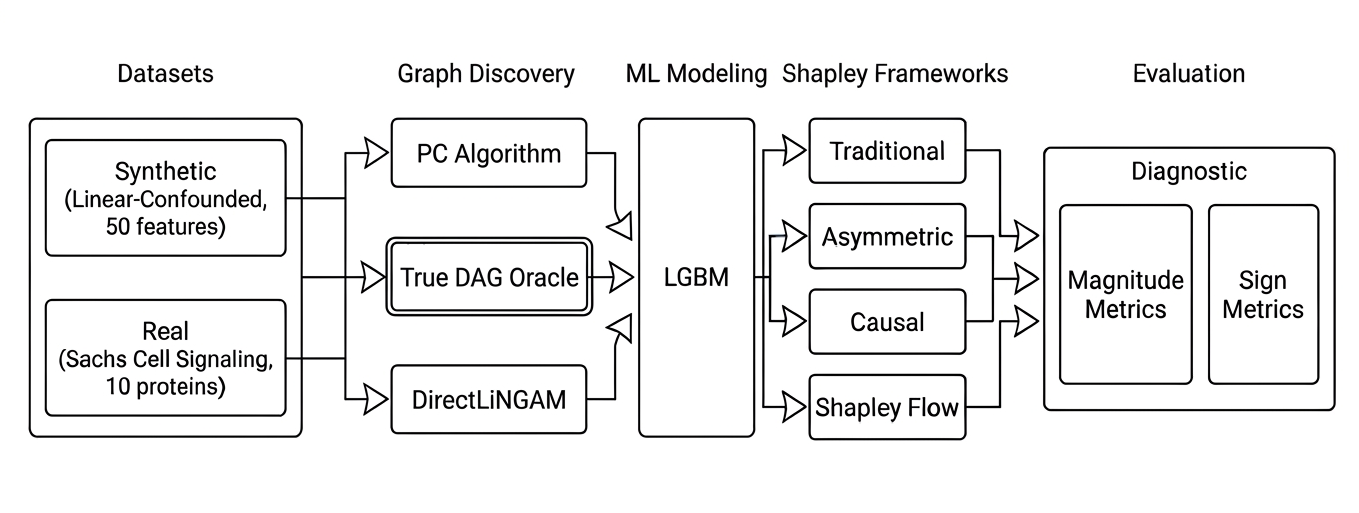
\includegraphics[width=\linewidth]{figures/experimental_pipeline_diagram.png}
  \caption{\textbf{Overview of the experimental pipeline.} End-to-end flow from data generation and causal discovery through Shapley computation to evaluation, illustrating how the two datasets, three graph sources, and three structure-aware methods feed into the magnitude and sign metrics.}
  \label{fig:pipeline}
\end{figure}

\subsection{Data Synthesis and Target Datasets}

The experimental pipeline employs a synthetic benchmarking framework to generate a dataset with a known, deterministic ground-truth causal structure. Specifically, the analysis in this thesis relies on a simulated linear system with confounding, paired alongside the real-world Sachs dataset. This linear configuration was selected because it closely matches the operating assumptions of the two discovery algorithms: both the PC algorithm and DirectLiNGAM are designed around linear structural relationships. By utilizing a linear data-generating process, the discovery task remains aligned with what these estimators can in principle recover, ensuring that the errors observed downstream can be attributed to confounding and finite-sample noise rather than a fundamental mismatch between the data and the estimators' functional assumptions. The deliberate addition of hidden confounders then violates the causal sufficiency assumption shared by both algorithms, providing precisely the stress condition of interest. The two core cases analyzed throughout the pipeline are therefore the following:

\paragraph{Linear System with Confounding (Synthetic).}
Strictly linear structural equations $X_j = \sum_{i \in \mathrm{Pa}(j)} w_{ij} X_i + \varepsilon_j$, with $\varepsilon_j \sim \mathcal{N}(0, 0.5)$ and coefficients drawn from $\mathrm{Uniform}(0.5, 2.0)$ with random sign. The graph is Erd\H{o}s--R\'{e}nyi with edge probability $p = 0.07$, yielding 87 $X \to X$ edges across 50 features (${\approx}1.74$ edges per node). Exactly 15 of 50 features are direct causal parents of $Y$ (\texttt{y\_parents\_ratio} $= 0.30$). Five hidden confounders each additively influence 2--3 features, violating causal sufficiency for both discovery algorithms. Dataset parameters: $N_{\mathrm{FEATURES}} = 50$, $N_{\mathrm{SAMPLES}} = 1000$, \texttt{random\_state} $= 42$.

\paragraph{Sachs Cell Signaling Dataset (Real Data).}
7,466 simultaneous measurements of 11 protein concentrations in stimulated human T-cells \citep{Sachs2005}, obtained from the Carnegie Mellon University Philosophy Department causal datasets repository \citep{Scheines2024}. Akt kinase (\texttt{akt}) is the regression target $Y$ and 10 proteins are input features (\texttt{raf, mek, plc, pip2, pip3, erk, pka, pkc, p38, jnk}). A consensus reference DAG has 17 $X \to X$ edges and 3 direct $X \to Y$ edges. Raw concentrations are preprocessed with a log1p transformation, followed by StandardScaler fit on the training partition only.

Both datasets use an 80/20 train/test split with random seed 42. The synthetic graph density ($\sim$7.1\%, 1.74 edges/node) was calibrated to match the Sachs network density, enabling direct comparison between the two experimental tracks.

\subsection{Predictive Model}

A LightGBM gradient-boosted tree regressor is fitted to each dataset using Optuna-based hyperparameter optimization (50 TPE trials, RMSE objective). Feature selection is disabled for both datasets so that all input features participate in the model, keeping the feature space consistent with the causal graph and Shapley computation.

\begin{table}[H]
  \centering
  \small
  \caption{\textbf{Predictive Model Performance and Output Distribution on Test Sets.} The output std $\hat{\sigma}$ is the standard deviation of the LightGBM predictions, used to normalise the magnitude metrics (Section~\ref{sec:metrics}). AU\,=\,Akt concentration units.}
  \label{tab:model_performance}
  \begin{tabular}{lrrrcc}
    \toprule
    \textbf{Dataset} & \textbf{R\textsuperscript{2}} & \textbf{RMSE} & \textbf{MAE}
      & \textbf{Output mean} & \textbf{Output std $\hat{\sigma}$} \\
    \midrule
    Linear-Conf (synthetic) & 0.900 & 1.72 & 1.36 & $\approx{-0.47}$ & 4.71 \\
    Sachs (real data)        & 0.679 & 88.78 & 17.82 & $\approx 81.2$ AU & 116.76 AU \\
    \bottomrule
  \end{tabular}
\end{table}

Beyond accuracy, $\hat{\sigma}$ is recorded as a first-class model summary because all magnitude metrics in Section~\ref{sec:metrics} are reported as a fraction of it. The two datasets live on incomparable raw scales ($\hat{\sigma} = 4.71$ for the synthetic target vs.\ $\hat{\sigma} = 116.76$ Akt units for Sachs); dividing by $\hat{\sigma}$ makes a Magnitude Divergence of 0.10 mean the same thing on both tracks --- a shift of 10\% of the model's explainable output spread. The formal justification for this choice of normaliser is given in Section~\ref{sec:metrics}.

\subsection{Causal Discovery Framework}

\subsubsection{DirectLiNGAM Integration}

The pipeline uses \texttt{causal-learn}'s DirectLiNGAM. The library outputs an adjacency matrix where \texttt{matrix[i,j]} is the coefficient of $X_j$ on $X_i$; the matrix is transposed before binarization. Edges with $|\mathrm{coefficient}| < 0.10$ are pruned.

\subsubsection{PC Algorithm Integration}

Constraint-based discovery uses \texttt{causal-learn}'s \texttt{pc} function with the Fisher-z test at $\alpha = 0.05$. Undirected edges in the resulting CPDAG are resolved by orienting them from the lower to the higher feature index. Cyclic edges introduced by this step are detected and removed.

\subsubsection{\texorpdfstring{$X \to Y$}{X→Y} Edge Augmentation Rule}

Both PC and LiNGAM operate on the $X$-only feature matrix and therefore produce no edges to $Y$. Because Shapley Flow requires at least one direct $X_i \to Y$ edge per feature to accumulate edge credit, an explicit augmentation step appends $X_i \to Y$ edges for every feature in the prediction model. In practice this connects all features to $Y$, since feature selection is disabled. The same rule is applied uniformly across all methods and to the True DAG reference graph.

\subsubsection{Discovery Performance}

\begin{figure}[H]
  \centering
  
\includegraphics[width=0.85\linewidth]{figures/discovery_vs_r2.png}
  \caption{\textbf{Causal discovery F1 ($X \to X$ edges) versus LightGBM test R\textsuperscript{2}, synthetic vs.\ Sachs.} Bars give PC and LiNGAM F1 on each dataset; the dashed line tracks model R\textsuperscript{2}. The discovery-quality ordering of the two algorithms reverses between tracks even as model fit declines from synthetic to real data.}
  \label{fig:discovery_r2}
\end{figure}

On the synthetic track, PC outperforms LiNGAM (F1: 0.567 vs.\ 0.250): conditional independence tests can partially block confounder-induced associations. LiNGAM reports 105 edges with only 24 correct and 81 false positives (precision 0.23, F1 0.25) because latent confounders violate its foundational assumption of mutually independent exogenous noise. On Sachs the ordering flips (F1: 0.326 vs.\ 0.167); log-transformed protein concentrations retain non-Gaussian residuals that LiNGAM can exploit. Notably, PC's output on Sachs required removing two cycles before yielding a valid DAG.

\subsection{Shapley Computation Settings}

Computing exact Shapley values requires evaluating every possible coalition of features, and for a 50-feature system this amounts to $2^{50}$ coalitions. The cost is severe even for the graph-free baseline, but it is compounded for the structure-aware methods: because they follow the DAG during the value computation, sampling interventional values along a topological order or activating edges in sequence, each coalition evaluation is itself more expensive than a single model call, so an exhaustive enumeration becomes outright unfeasible in practice. For this reason every Shapley method in this pipeline, the graph-free baseline included, is computed with the same Monte Carlo permutation approximation rather than by exact enumeration, using $T = 100$ sampled permutations. For each dataset, 30\% of training rows serve as the background reference distribution (240 rows for synthetic; 1,791 for Sachs), and up to 100 test instances are explained. All random operations use seed 42.

Ten combinations of structure-aware Shapley method and causal graph are computed for the synthetic dataset: Traditional Shapley (baseline) plus the three structure-aware methods applied to three graph sources (PC, LiNGAM, True DAG). The Sachs dataset mirrors this design: Traditional Shapley plus the three methods applied to PC, LiNGAM, and the consensus reference DAG, which here serves the same oracle role that the True DAG plays on the synthetic track. The consensus Sachs graph is thus used both for evaluating discovery quality (Figure~\ref{fig:discovery_r2}) and as the oracle Shapley input against which the discovered-graph attributions are compared. The same $T = 100$ permutation budget is applied to every combination on both tracks.

Table~\ref{tab:method_comparison} summarizes what each method changes relative to Traditional Shapley. It is designed to be read one row at a time: each structure-aware method modifies exactly one ingredient of the Traditional recipe. Asymmetric Shapley changes only the permutation space; Causal Shapley changes only the value function, with the ordering following from the components; and Shapley Flow changes who the players are.

\begin{table}[H]
  \centering
  \caption{\textbf{What Each Method Changes Relative to Traditional Shapley.}}
  \label{tab:method_comparison}
  \footnotesize
  \begin{tabularx}{\textwidth}{p{2.6cm}XXXX}
    \toprule
    \textbf{Property} & \textbf{Traditional} & \textbf{Asymmetric} & \textbf{Causal} & \textbf{Flow} \\
    \midrule
    Players & Features & Features & Features & Edges \\
    Permutation space & All $N!$ orderings & Topological orderings of feature DAG & Topological orderings of component DAG & All orderings of edge set \\
    Value function & Obs.\ $\mathbb{E}[f \mid X_S{=}x_S]$ & Observational (same) & Interventional $\mathbb{E}[f \mid \mathrm{do}(X_S{=}x_S)]$ & Foreground/background by edge activation \\
    Graph's role & None & Constrains ordering & Defines components, ordering, and intervention & Supplies the players (edges) \\
    \bottomrule
  \end{tabularx}
\end{table}

\subsubsection{Traditional Shapley Values (Graph-Free Baseline)}

The baseline discards all causal information. All features are treated symmetrically: $T = 100$ uniformly random permutations of all features are sampled and, building each coalition incrementally, the marginal contribution of each feature is computed by replacing the absent features with values drawn from the background data. This is the standard SHAP Monte Carlo estimator \citep{Lundberg2017} and serves as the graph-free reference against which all structure-aware methods are benchmarked.

The coalition value $v(S) = \mathbb{E}[f(X) \mid X_S = x_S]$ is estimated by the \textsc{coalition\_value} subroutine (Appendix~\ref{app:subroutines}), which overwrites the coalition columns of the background matrix with the instance's real values and averages the model output, and which is reused unchanged by Asymmetric Shapley.

\begin{algorithm}[H]
  \caption{Traditional Shapley (Monte Carlo)}
  \label{alg:traditional}
  \begin{algorithmic}[1]
    \INPUT{instance $x$, model $f$, background data $D$, number of permutations $T$}
    \OUTPUT{attribution vector $\phi \in \mathbb{R}^n$}
    \State $\phi \gets \mathbf{0}_n$
    \State $\text{baseline} \gets \text{mean}(f(D))$  \Comment{$v(\emptyset)$: all features marginalised}
    \For{$t = 1 \ldots T$}
      \State $\pi \gets \textsc{random\_permutation}(1 \ldots n)$  \Comment{unconstrained uniform ordering}
      \State $S \gets \emptyset$,\quad $v_{\text{prev}} \gets \text{baseline}$
      \For{$i$ \textbf{in} $\pi$}  \Comment{add features one at a time}
        \State $S \gets S \cup \{i\}$
        \State $v_{\text{curr}} \gets \textsc{coalition\_value}(x, S, f, D)$
        \State $\phi[i] \gets \phi[i] + (v_{\text{curr}} - v_{\text{prev}})$
        \State $v_{\text{prev}} \gets v_{\text{curr}}$
      \EndFor
    \EndFor
    \Return $\phi \mathbin{/} T$
  \end{algorithmic}
\end{algorithm}

The graph is never consulted, which is the defining property of the method. The cost is $O(T \cdot n \cdot |D|)$ model rows evaluated per instance.

\subsubsection{Asymmetric Shapley Values}

The Asymmetric Shapley implementation retains the same observational coalition value as Traditional Shapley but replaces the uniform random permutation with a randomized Kahn topological sort that draws uniformly from the linear extensions of the feature DAG (the \textsc{sample\_topological\_ordering} subroutine, Appendix~\ref{app:subroutines}). The modification is exclusively in the permutation space; the coalition values are computed identically through \textsc{coalition\_value}. The children lists and initial in-degrees are precomputed once over the $X$-only subgraph, since $Y$ is never a player; if the feature DAG contains a cycle the constraints are disabled and the method reduces to Traditional Shapley.

\begin{algorithm}[H]
  \caption{Asymmetric Shapley}
  \label{alg:asymmetric}
  \begin{algorithmic}[1]
    \INPUT{instance $x$, model $f$, background data $D$, feature DAG $G$, permutations $T$}
    \OUTPUT{attribution vector $\phi \in \mathbb{R}^n$}
    \PRECOMPUTE \texttt{children[]}, \texttt{in\_degree[]} from the $X$-only edges of $G$  (Subroutine~\ref{alg:topo})
    \State $\phi \gets \mathbf{0}_n$,\quad $\text{baseline} \gets \text{mean}(f(D))$
    \For{$t = 1 \ldots T$}
      \State $\pi \gets \textsc{sample\_topological\_ordering}()$  \Comment{ancestors precede descendants}
      \State $S \gets \emptyset$,\quad $v_{\text{prev}} \gets \text{baseline}$
      \For{$i$ \textbf{in} $\pi$}
        \State $S \gets S \cup \{i\}$
        \State $v_{\text{curr}} \gets \textsc{coalition\_value}(x, S, f, D)$  \Comment{same value fn as Traditional}
        \State $\phi[i] \gets \phi[i] + (v_{\text{curr}} - v_{\text{prev}})$
        \State $v_{\text{prev}} \gets v_{\text{curr}}$
      \EndFor
    \EndFor
    \Return $\phi \mathbin{/} T$
  \end{algorithmic}
\end{algorithm}

The cost is the same order as Traditional Shapley; the topological sampler adds only $O(n)$ per permutation. The graph is consulted solely to build the ordering structures at initialization, and the value function never sees it.

\subsubsection{Causal Shapley Values}

Causal Shapley replaces the observational coalition value with post-interventional sampling that approximates Pearl's do-operator, $v_{\mathrm{do}}(S) = \mathbb{E}[f(X) \mid \mathrm{do}(X_S = x_S)]$. The method has two nested levels of stochasticity that must be kept distinct: an outer loop that draws a fresh uniform linear extension of the component DAG for each Shapley trial, and an inner loop that, for each coalition, estimates the interventional value from $M$ draws of the post-interventional distribution while traversing components in a fixed deterministic topological order so that each node's parents are resolved before the node itself. Each draw fixes the intervened features and fills in the remaining features from their parents using the closed-form conditional Gaussian of the background data; inside a confounded component the missing features are drawn independently given their parents (which destroys the spurious within-component correlation), while in an ordinary component they are drawn jointly given the parents and any fixed siblings. In this pipeline the confounder list is empty, so every feature is its own component, the outer ordering reduces to a uniform linear extension of the full feature DAG, and the inner sampler always takes the univariate-Gaussian branch. The experiments use $T = 100$ outer permutations and $M = 10$ inner samples.

\begin{algorithm}[H]
  \caption{Causal Shapley (post-interventional)}
  \label{alg:causal}
  \begin{algorithmic}[1]
    \INPUT{instance $x$, model $f$, background data $D$, feature adjacency $A$ ($X$ only),}
    \Statex \hspace{2.5em} confounder list, outer permutations $T$, inner samples $M$
    \OUTPUT{attribution vector $\phi \in \mathbb{R}^n$}
    \PRECOMPUTE \texttt{components}, \texttt{confounded[]}, \texttt{parents[]} $\gets$ \textsc{build\_components}$(A, \text{confounder list})$
    \State $\mu \gets \text{mean}(D)$;\quad $\Sigma \gets \text{cov}(D) + \varepsilon I$  \Comment{$\varepsilon$ for numerical stability}
    \State $\phi \gets \mathbf{0}_n$,\quad $\text{baseline} \gets \text{mean}(f(D))$
    \For{$t = 1 \ldots T$}  \Comment{OUTER: re-randomised}
      \State $\pi \gets \textsc{sample\_component\_topo\_ordering}()$, then expand to features
      \State $S \gets \emptyset$,\quad $v_{\text{prev}} \gets \text{baseline}$
      \For{$i$ \textbf{in} $\pi$}
        \State $S \gets S \cup \{i\}$
        \State $v_{\text{curr}} \gets 0$  \Comment{INNER: estimate $v_{\mathrm{do}}$}
        \For{$m = 1 \ldots M$}
          \State $v_{\text{curr}} \gets v_{\text{curr}} + f(\textsc{post\_interventional\_sample}(x, S, \ldots))$
        \EndFor
        \State $v_{\text{curr}} \gets v_{\text{curr}} \mathbin{/} M$
        \State $\phi[i] \gets \phi[i] + (v_{\text{curr}} - v_{\text{prev}})$
        \State $v_{\text{prev}} \gets v_{\text{curr}}$
      \EndFor
    \EndFor
    \Return $\phi \mathbin{/} T$
  \end{algorithmic}
\end{algorithm}

The \textsc{post\_interventional\_sample} subroutine that draws a single sample from $P(X \mid \mathrm{do}(X_S = x_S))$, together with the closed-form conditional-Gaussian draw it relies on, is given in Appendix~\ref{app:subroutines}.

The cost is $O(T \cdot n \cdot M)$ model evaluations, markedly heavier than Traditional or Asymmetric Shapley because of the inner sampling loop. The graph is used in three places: the directed edges define the parent sets for the interventional draws, the edges plus the confounder list define the component partition and the component DAG that constrains the outer ordering, and the same DAG fixes the deterministic inner traversal order.

\subsubsection{Shapley Flow}
\label{sec:flow_alg}

Shapley Flow treats directed edges as the players of the cooperative game, permuting the full edge set rather than the feature set. In each of $T = 100$ trials all edges ($X \to X$ and $X \to Y$) are randomly permuted and activated sequentially, and the system value is evaluated after each activation. The node-value assignment is binary: a node takes its foreground value if it is a source with an active outgoing edge, or if it has an active incoming edge, or if its direct edge to $Y$ is active; otherwise it takes its background value, and $Y$ is always dropped before the model is evaluated. No intermediate model calls are made between $X$ features; the model is evaluated only on the complete node-value vector at each edge addition. Node-level attributions are recovered by summing each node's outgoing edge credits, and by construction the credits satisfy efficiency, summing to $f(x_{\mathrm{fg}}) - f(x_{\mathrm{bg}})$. The $X \to Y$ augmentation of Section~\ref{sec:setup} is essential here, as it guarantees every feature has a direct route to accumulate edge credit.

\begin{algorithm}[H]
  \caption{Shapley Flow (uniform edge-permutation)}
  \label{alg:flow}
  \begin{algorithmic}[1]
    \INPUT{foreground instance $x_{\mathrm{fg}}$, background row $x_{\mathrm{bg}}$,}
    \Statex \hspace{2.5em} graph adjacency ($n+1$ nodes incl.\ $Y$), target index $Y$, trials $T$
    \OUTPUT{node attribution vector $\phi \in \mathbb{R}^n$ ($Y$ excluded)}
    \State $E \gets \text{list of all directed edges } (u \to v) \text{ in the graph}$
    \State $\texttt{edge\_credit} \gets \{e: 0.0 \mid e \in E\}$
    \For{$t = 1 \ldots T$}
      \State $\text{perm} \gets \textsc{random\_permutation}(E)$  \Comment{unconstrained over ALL edges}
      \State $v_{\text{prev}} \gets \textsc{system\_value}(\emptyset, x_{\mathrm{fg}}, x_{\mathrm{bg}})$  \Comment{$= f(x_{\mathrm{bg}})$}
      \State $\text{active} \gets []$
      \For{$e$ \textbf{in} $\text{perm}$}
        \State $\text{active}.\text{append}(e)$
        \State $v_{\text{curr}} \gets \textsc{system\_value}(\text{active}, x_{\mathrm{fg}}, x_{\mathrm{bg}})$
        \State $\texttt{edge\_credit}[e] \gets \texttt{edge\_credit}[e] + (v_{\text{curr}} - v_{\text{prev}})$
        \State $v_{\text{prev}} \gets v_{\text{curr}}$
      \EndFor
    \EndFor
    \For{$e \in E$}\quad $\texttt{edge\_credit}[e] \gets \texttt{edge\_credit}[e] \mathbin{/} T$\EndFor
    \State $\phi \gets \mathbf{0}_n$  \Comment{aggregate edges $\to$ features}
    \For{each edge $(u \to v) \in E$}
      \If{$u \neq Y$}\quad $\phi[u] \gets \phi[u] + \texttt{edge\_credit}[(u \to v)]$\EndIf
    \EndFor
    \Return $\phi$
  \end{algorithmic}
\end{algorithm}

The \textsc{system\_value} subroutine that maps a set of active edges to a model prediction, by assigning each node its foreground or background value under the activation rule, is given in Appendix~\ref{app:subroutines}.

The cost is $T \cdot (|E| + 1)$ model evaluations per instance (for the synthetic system, roughly $50 \times 276 \approx 1.4 \times 10^4$). This is the most structure-dependent of the four methods: the graph supplies the players themselves, so with no graph there is no game to play.

\subsection{Evaluation Metrics}
\label{sec:metrics}

\subsubsection{Notation}

Let $N$ be the number of input features, $\mathcal{F} = \{1,\ldots,N\}$ the feature index set, and $\mathcal{I}$ the set of test instances. The trained predictive model is $f: \mathbb{R}^N \to \mathbb{R}$, and $\hat{\sigma} = \mathrm{std}_{i \in \mathcal{I}}\, f(x_i)$ is the standard deviation of its predictions over the test set, the natural scale of the attribution space, so every magnitude number in this chapter is reported as a fraction of it. Let $m \in \{\text{Traditional, Asymmetric, Causal, Flow}\}$ index the Shapley method and $G \in \{\emptyset, \text{PC}, \text{LiNGAM}, \text{True DAG}\}$ the causal graph source.

The per-instance per-feature attribution $\phi^{m,G}_{i,f}$ is the Shapley value assigned to feature $f \in \mathcal{F}$ for instance $i \in \mathcal{I}$ by method $m$ using graph $G$. Every comparison fixes a subject $(m, G)$ with $G \in \{\text{PC}, \text{LiNGAM}\}$ and contrasts it against one of three reference configurations: the \textbf{baseline} ref (Traditional Shapley, $G = \emptyset$, graph-free baseline), the \textbf{oracle} ref (True DAG on synthetic, consensus DAG on Sachs), and the \textbf{cross-discovery} ref (same method on the opposite discovered graph, $\text{PC} \leftrightarrow \text{LiNGAM}$).

\subsubsection{Two Dimensions, Two Metrics, Three Comparisons}

Every comparison in this chapter asks the same two questions of a (method, graph) result against a reference: did the attribution change in \textbf{magnitude}, and did it change in \textbf{direction}? These are the two evaluation dimensions, and each is measured by a single metric used identically in all three comparisons:

\begin{itemize}[nosep]
  \item \textbf{Magnitude Divergence ($\Delta M$)}: how much the absolute attribution moves relative to the reference, expressed as a fraction of $\hat{\sigma}$. $\Delta M \geq 0$; $\Delta M = 0.10$ means the typical attribution shifted by 10\% of $\hat{\sigma}$.
  \item \textbf{Sign Disagreement ($D$)}: the fraction of (instance, feature) attributions that point in the opposite direction to the reference. $D \in [0, 1]$; $D = 0$ means perfect directional agreement.
\end{itemize}

The only thing that changes between comparisons is the reference, which is carried as a tag so the same two names cover all six cells of Table~\ref{tab:metric_framework}:
\begin{itemize}[nosep]
  \item Tag \textbf{base} --- reference is Traditional Shapley (how far a graph moves attributions away from the graph-free baseline); Section~\ref{sec:baseline}.
  \item Tag \textbf{oracle} --- reference is the True / consensus DAG (how faithfully a discovered graph recovers the oracle attributions); Section~\ref{sec:oracle_align}.
  \item Tag \textbf{disc} --- reference is the opposite discovered graph (how much the choice of discovery algorithm alone perturbs attributions); Section~\ref{sec:disc_analysis}.
\end{itemize}

\begin{table}[H]
  \centering
  \caption{\textbf{Evaluation Metric Framework.} Two metrics, two dimensions, three reference comparisons.}
  \label{tab:metric_framework}
  \begin{tabularx}{\textwidth}{lXXX}
    \toprule
    \textbf{Dimension} & \textbf{vs.\ Traditional (base)} & \textbf{vs.\ Oracle DAG (oracle)} & \textbf{PC vs.\ LiNGAM (disc)} \\
    \midrule
    Magnitude  & $\Delta M_{\text{base}}$   & $\Delta M_{\text{oracle}}$   & $\Delta M_{\text{disc}}$   \\
    Sign / Dir & $D_{\text{base}}$          & $D_{\text{oracle}}$          & $D_{\text{disc}}$          \\
    \bottomrule
  \end{tabularx}
\end{table}

\subsubsection{Three Measurement Levels}

Both metrics are defined once at the atomic instance level and then lifted to the feature and global levels by fixed aggregation operators, so a single definition serves all three reporting granularities. The level is stated wherever a value is reported; as a convention, tables give the global level, heatmaps the feature level, and scatter plots the instance level.

\paragraph{Instance level (signed).}
The atomic magnitude quantity is the signed gap between absolute attributions for one (instance, feature):
\begin{equation}
  \delta^{\mathrm{ref}}_{i,f} = \left|\phi^{m,G}_{i,f}\right| - \left|\phi^{\mathrm{ref}}_{i,f}\right|.
\end{equation}
This keeps its sign on purpose: a positive value means the discovered graph inflates the feature's local importance relative to the reference, a negative value means it suppresses it. The atomic sign quantity is the disagreement indicator $\mathbf{1}\!\left[\operatorname{sign}(\phi^{m,G}_{i,f}) \neq \operatorname{sign}(\phi^{\mathrm{ref}}_{i,f})\right]$, defined only on instances where the reference attribution is non-zero.

\paragraph{Feature level (non-negative).}
Per feature, the instance gaps are collapsed by a root-mean-square over instances and normalised by $\hat{\sigma}$:
\begin{equation}
  \Delta M^{\mathrm{ref}}_f = \frac{1}{\hat{\sigma}}\sqrt{\frac{1}{|\mathcal{I}|}\sum_{i \in \mathcal{I}} \left(\delta^{\mathrm{ref}}_{i,f}\right)^2}.
\end{equation}
The RMS (rather than a plain mean) measures the typical size of the per-instance change without letting positive and negative gaps cancel, and dividing by $\hat{\sigma}$ puts the result on a single interpretable scale (percentage of model-output standard deviation) that is comparable across features and across datasets of different raw units.

The choice of $\hat{\sigma}$ as that scale is not arbitrary; it is the natural unit of the attribution space itself. By the efficiency axiom, every Shapley method here satisfies $\sum_{f} \phi^{m,G}_{i,f} = f(x_i) - \mathbb{E}[f(x)]$, so the attributions live on the same scale as the model output and $\hat{\sigma} = \mathrm{std}_{i}\, f(x_i)$ is the total dispersion the whole SHAP space has to distribute. Normalising by $\hat{\sigma}$ expresses a magnitude change as a fraction of the attribution budget that actually exists, a value of 0.10 means ``a tenth of the model's explainable variation'' regardless of whether the target is a unitless synthetic variable or a raw protein concentration.

The feature-level sign metric is the disagreement rate $D^{\mathrm{ref}}_f$, the fraction of valid instances whose sign disagrees with the reference.

\paragraph{Global level.}
Both feature-level metrics are averaged over features:
\begin{equation}
  \Delta M^{\mathrm{ref}} = \frac{1}{N}\sum_{f \in \mathcal{F}} \Delta M^{\mathrm{ref}}_f,
  \qquad
  D^{\mathrm{ref}} = \frac{1}{N}\sum_{f \in \mathcal{F}} D^{\mathrm{ref}}_f.
\end{equation}

The cross-discovery metrics $\Delta M_{\text{disc}}$ and $D_{\text{disc}}$ are the same constructions with the subject fixed to PC and the reference to LiNGAM.

%% ============================================================
\section{Results and Empirical Analysis}
\label{sec:results}
%% ============================================================

\subsection{Causal Discovery Baseline Performance}

\subsubsection{Performance on the Confounded Linear System}

The five hidden confounders introduce spurious correlations that directly violate the causal sufficiency assumption of both estimators. PC exhibits high structural resilience, recovering 40 of 87 true $X \to X$ edges with precision 0.741 and F1 of 0.567. Thanks to conditional independence testing, which evaluates localized relationships, it can partially block extended confounder-induced association paths through careful conditioning on intermediate variables \citep{Spirtes2000}, allowing PC to maintain a structurally conservative graph relatively close to the true sparse structure.

DirectLiNGAM experiences severe structural degradation, reporting 105 edges with only 24 correct and 81 false positives (precision 0.23, F1 0.25). Standard linear non-Gaussian functional models are highly sensitive to unmeasured variables; because latent confounders violate the foundational assumption of mutually independent exogenous noise, the algorithm frequently misinterprets confounder-induced correlations as direct causal pathways \citep{Hoyer2008, Shimizu2011}. This over-discovery creates the central experimental contrast: the same Shapley methods receive fundamentally different structural priors from the two discovery algorithms.

\begin{figure}[H]
  \centering
  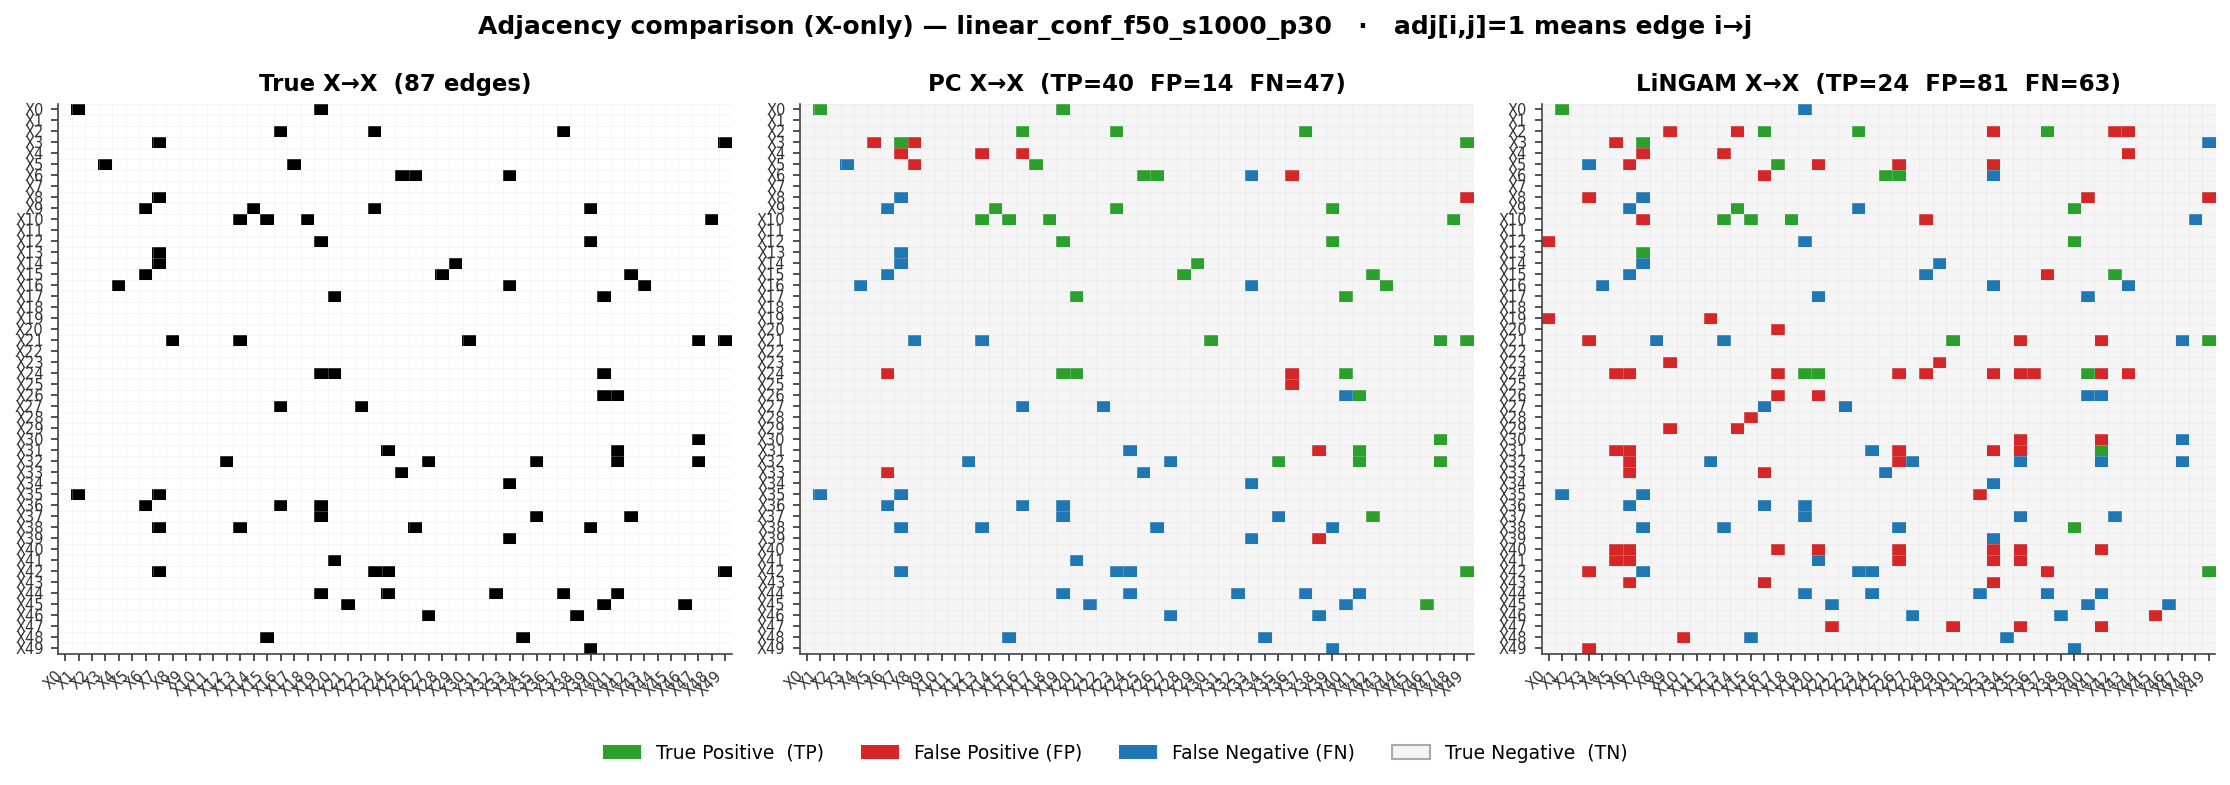
\includegraphics[width=\linewidth]{figures/adjacency_comparison_linear_conf_f50_s1000_p30.png}
  \caption{\textbf{$X \to X$ adjacency matrices for the synthetic linear-confounded dataset, where $\mathrm{adj}[i,j]=1$ denotes an edge $i \to j$.} The True DAG (87 edges) is shown alongside the PC (54 edges) and LiNGAM (105 edges) recoveries. PC stays close to the sparse true structure, whereas LiNGAM scatters spurious edges across the matrix, the visual signature of the over-connection that drives its low precision.}
  \label{fig:adj_synthetic}
\end{figure}

\subsubsection{Performance Reversal on the Sachs Cell Signaling Dataset}

On the real-world Sachs dataset, the performance hierarchy reverses: LiNGAM outperforms PC (F1 = 0.326 vs.\ 0.167; precision = 0.269 vs.\ 0.158). Real intracellular signaling pathways generate joint distributions with strong non-Gaussian marginals even after log1p transformation, a property that LiNGAM's functional causal model is explicitly designed to exploit. Conversely, PC's Fisher-z test assumes linear, multivariate Gaussian residuals. This introduces a known sample-size paradox: while larger sample sizes generally improve causal discovery, providing PC with a massive biological dataset (5,972 training rows compared to 800 in the synthetic side) gives the statistical tests so much power that they become hypersensitive to minor non-Gaussian distributional violations \citep{Glymour2019, Ramsey2014}. Consequently, PC loses its discriminative thresholding power under this physical complexity, leading to severe under-recovery.

\begin{figure}[H]
  \centering
  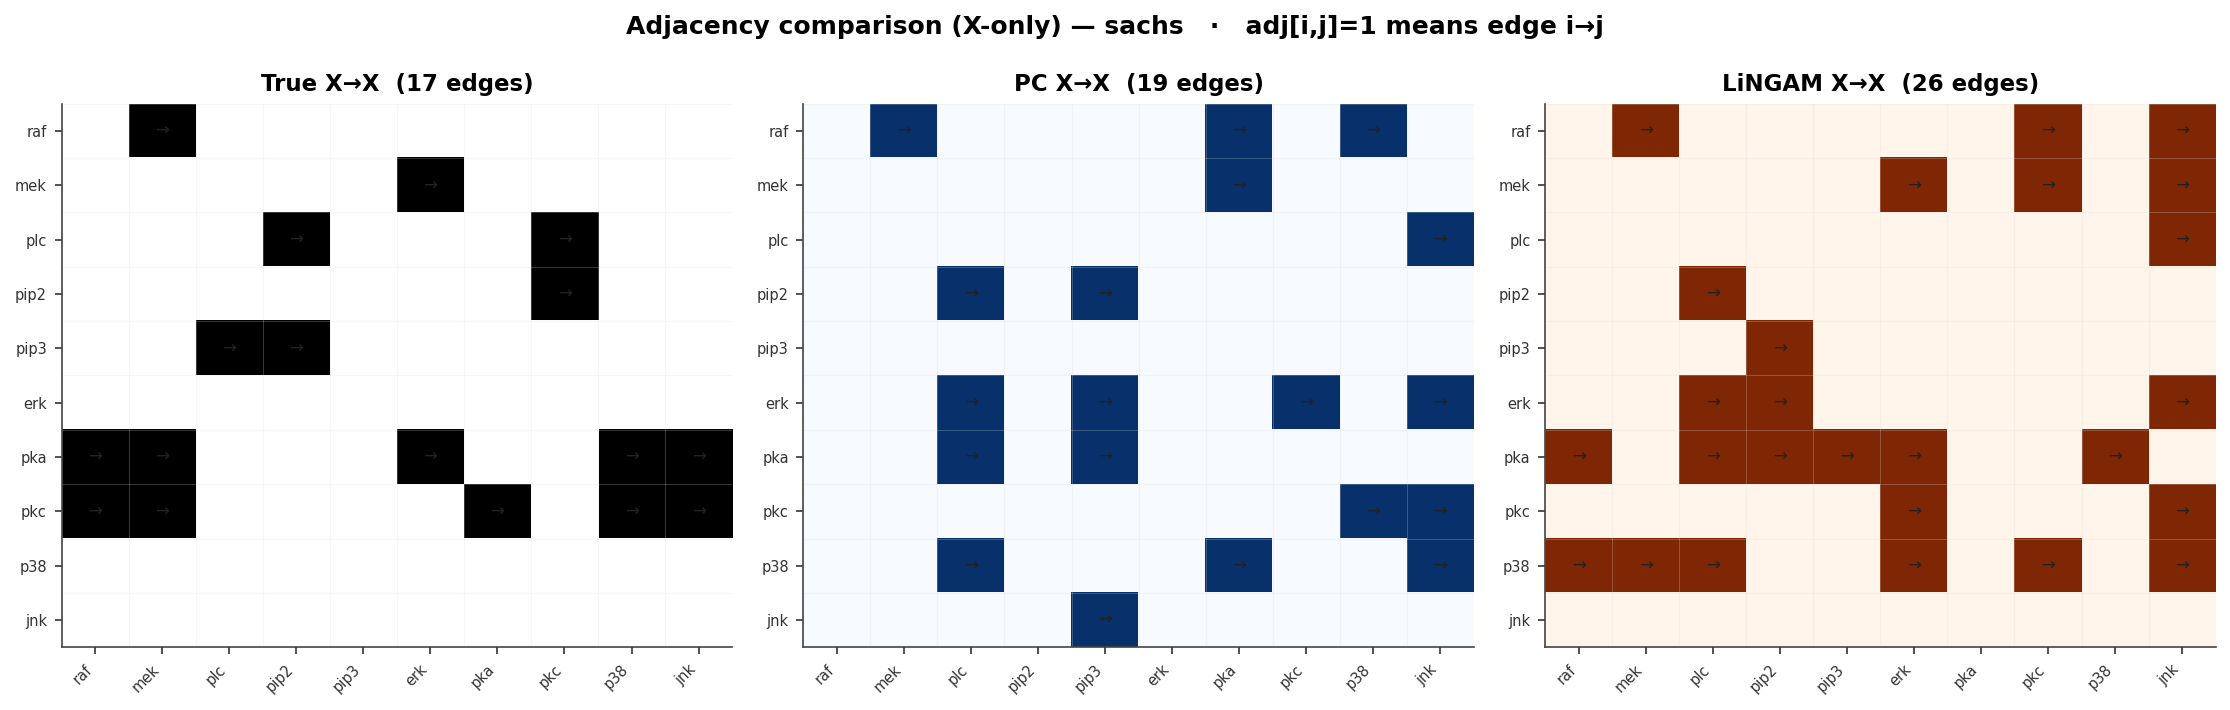
\includegraphics[width=\linewidth]{figures/adjacency_comparison_sachs.png}
  \caption{\textbf{$X \to X$ adjacency matrices for the Sachs dataset, where $\mathrm{adj}[i,j]=1$ denotes an edge $i \to j$.} The consensus reference DAG (17 edges) is compared against the PC (19 edges) and LiNGAM (26 edges) recoveries over the ten signaling proteins. Both algorithms recover only a fraction of the true links and introduce edges absent from the consensus network, with LiNGAM the denser of the two.}
  \label{fig:adj_sachs}
\end{figure}

\subsection{Graph-Free Baseline Deviation Analysis}
\label{sec:baseline}

Following the metric definitions of Section~\ref{sec:metrics}, this evaluation block compares each structure-aware method and discovered-graph combination against the Traditional Shapley baseline ($\Delta M_{\text{base}}$, $D_{\text{base}}$) to verify the expected theoretical behaviour of each method and validate that this behaviour holds on real data.

The theoretical ordering of sensitivity to causal graph injection is given directly by Table~\ref{tab:method_comparison}. Asymmetric Shapley is the least conditioned by the graph: it uses the discovered edges only to restrict the permutation space while keeping the observational value function unchanged, so its deviation from the graph-free baseline depends entirely on how many orderings the graph forbids. Causal Shapley is more sensitive: the graph enters the value function itself, driving post-interventional distributions for features outside the coalition via their discovered parent sets, so every false or missing edge corrupts an attribution directly. Shapley Flow is the most sensitive: the discovered edges are the players of the game, and the entire credit-routing mechanism collapses without them, so any graph error propagates across all downstream paths simultaneously.

Two cross-cutting patterns emerge from Tables~\ref{tab:baseline_synth}--\ref{tab:baseline_sachs} and are visible immediately in the scatter plots. First, Sign Disagreement $D_{\text{base}}$ is a more pervasive perturbation than Magnitude Divergence $\Delta M_{\text{base}}$: introducing a causal graph flips the direction of a larger share of feature attributions than it inflates their absolute size. This is because sign inversions arise whenever a moderate per-feature change crosses zero, a threshold many near-zero attributions sit close to, while large magnitude changes are concentrated in a handful of dominant features. Second, the choice of discovered graph---PC or LiNGAM---matters little for the graph-versus-no-graph contrast: both discovered graphs perturb $\Delta M_{\text{base}}$ and $D_{\text{base}}$ by nearly identical amounts for a given method, so the dominant driver of deviation is the method's structural coupling to any causal graph, not the specific graph supplied.

\begin{figure}[H]
  \centering
  \begin{subfigure}[t]{0.48\linewidth}
    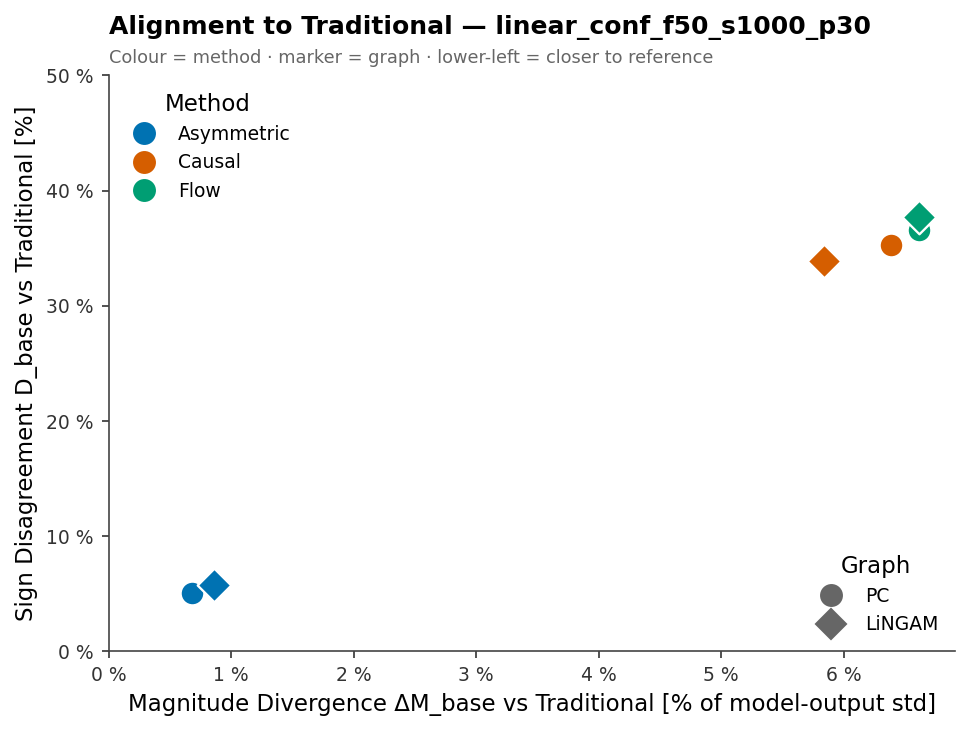
\includegraphics[width=\linewidth]{figures/tga_sa_scatter_traditional_linear_conf_f50_s1000_p30.png}
    \caption{Synthetic dataset. Asymmetric Shapley clusters tightly in the lower-left corner under both graphs, while Causal and Flow sit far to the upper-right, deviating strongly on both axes regardless of which graph supplies the structure.}
    \label{fig:scatter_trad_synth}
  \end{subfigure}
  \hfill
  \begin{subfigure}[t]{0.48\linewidth}
    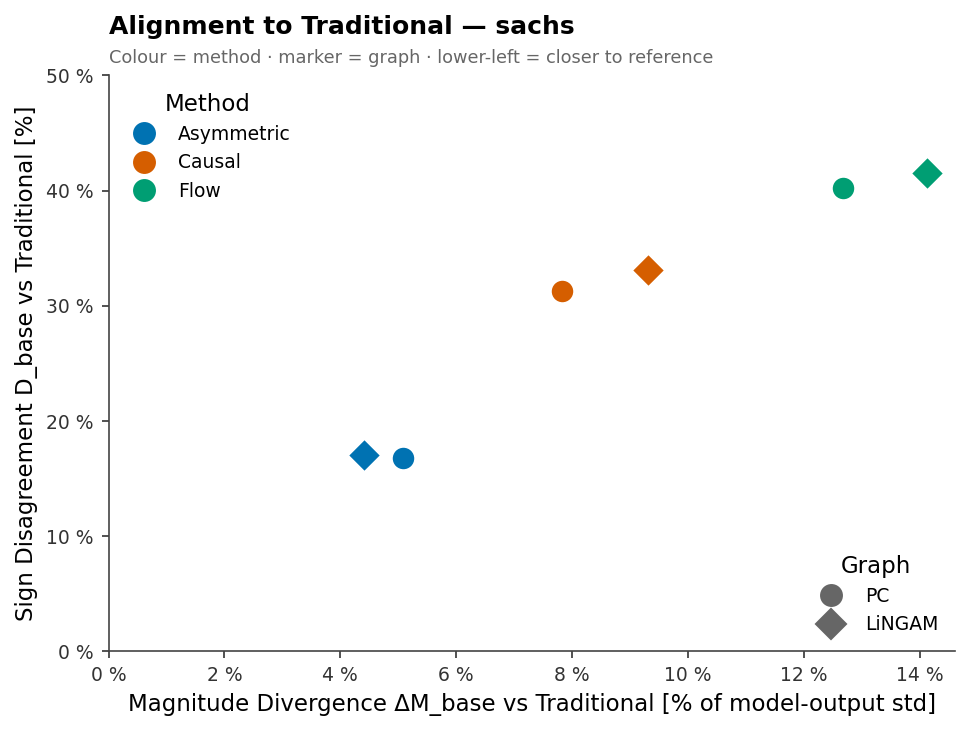
\includegraphics[width=\linewidth]{figures/tga_sa_scatter_traditional_sachs.png}
    \caption{Sachs dataset. The same lower-left clustering of Asymmetric Shapley holds, but both axes spread wider than on synthetic and the PC/LiNGAM markers separate more visibly for Causal and Flow, but still less than 2\% apart, the early signal of the discovery-algorithm sensitivity examined in Section~\ref{sec:disc_analysis}.}
    \label{fig:scatter_trad_sachs}
  \end{subfigure}
  \caption{\textbf{Magnitude versus sign deviation from Traditional Shapley.}}
  \label{fig:scatter_trad}
\end{figure}

\begin{table}[H]
  \centering
  \caption{\textbf{Baseline Deviation -- Linear-Conf Synthetic Dataset.}}
  \label{tab:baseline_synth}
  \begin{tabular}{llrr}
    \toprule
    \textbf{Method} & \textbf{Graph} & $D_{\text{base}}$ & $\Delta M_{\text{base}}$ \\
    \midrule
    Asymmetric & PC     & 5.08\%  & 0.68\% \\
    Asymmetric & LiNGAM & 5.76\%  & 0.86\% \\
    Causal     & PC     & 35.30\% & 6.39\% \\
    Causal     & LiNGAM & 33.92\% & 5.84\% \\
    Flow       & PC     & 36.58\% & 6.62\% \\
    Flow       & LiNGAM & 37.68\% & 6.61\% \\
    \bottomrule
  \end{tabular}
\end{table}

\begin{table}[H]
  \centering
  \caption{\textbf{Baseline Deviation -- Sachs Cell Signaling Dataset.}}
  \label{tab:baseline_sachs}
  \begin{tabular}{llrr}
    \toprule
    \textbf{Method} & \textbf{Graph} & $D_{\text{base}}$ & $\Delta M_{\text{base}}$ \\
    \midrule
    Asymmetric & PC     & 16.80\% & 5.08\%  \\
    Asymmetric & LiNGAM & 17.00\% & 4.41\%  \\
    Causal     & PC     & 31.30\% & 7.83\%  \\
    Causal     & LiNGAM & 33.10\% & 9.31\%  \\
    Flow       & PC     & 40.20\% & 12.68\% \\
    Flow       & LiNGAM & 41.50\% & 14.17\% \\
    \bottomrule
  \end{tabular}
\end{table}

\begin{figure}[H]
  \centering
  \begin{subfigure}[t]{0.48\linewidth}
    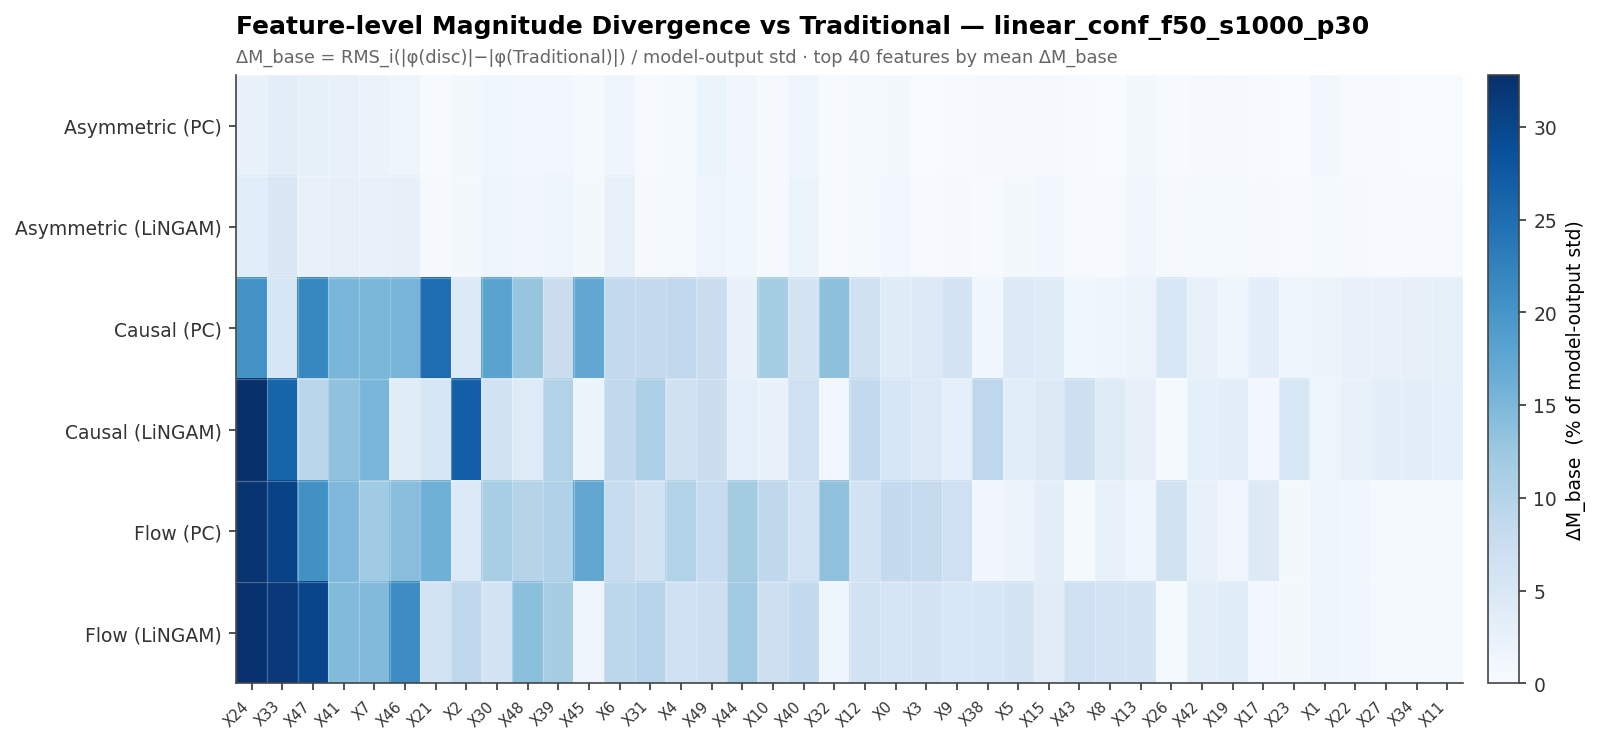
\includegraphics[width=\linewidth]{figures/tga_heatmap_traditional_linear_conf_f50_s1000_p30.png}
    \caption{Synthetic dataset (top 10 features by mean $\Delta M_{\text{base}}$). Rows are method-graph combinations; columns are features. The Asymmetric rows are near-zero throughout, while Causal and Flow concentrate their largest deviations on X24, X33 and X47.}
    \label{fig:heatmap_trad_synth}
  \end{subfigure}
  \hfill
  \begin{subfigure}[t]{0.48\linewidth}
    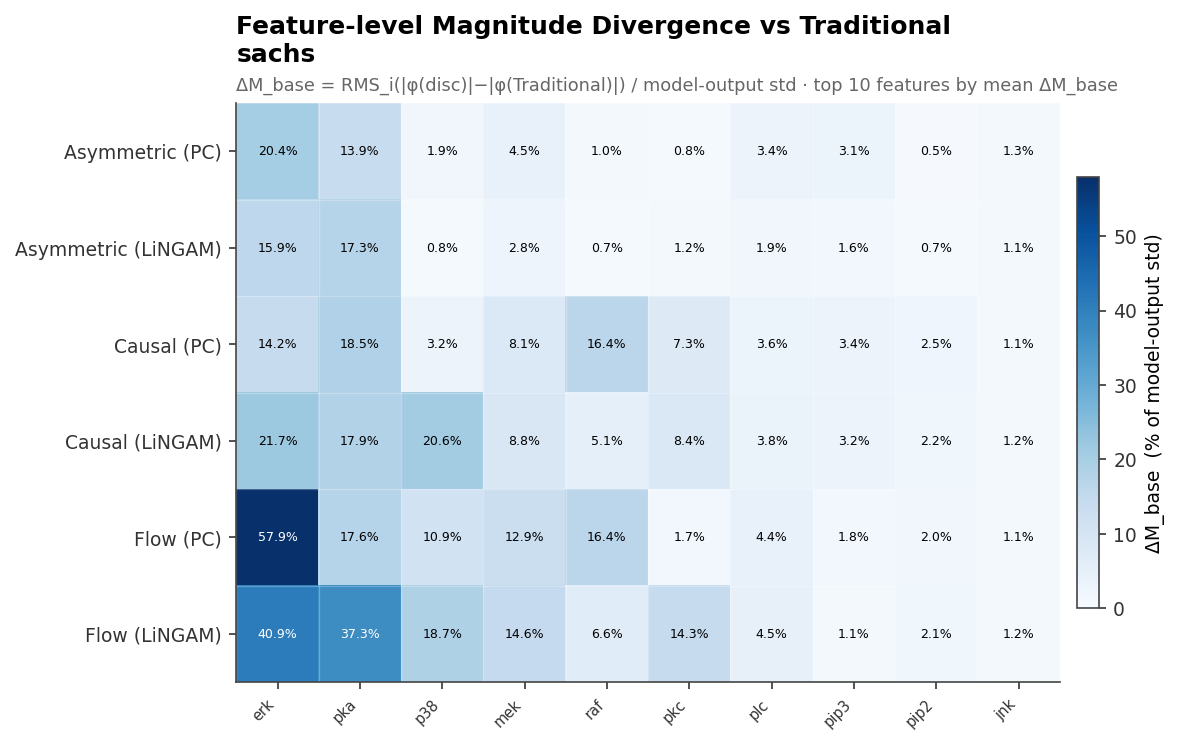
\includegraphics[width=\linewidth]{figures/tga_heatmap_traditional_sachs.png}
    \caption{Sachs dataset (top 10 features by mean $\Delta M_{\text{base}}$). The deviation concentrates on erk and pka, with Flow under PC producing the single largest feature-level shift (erk, 57.9\% of $\hat{\sigma}$).}
    \label{fig:heatmap_trad_sachs}
  \end{subfigure}
  \caption{\textbf{Feature-level Magnitude Divergence $\Delta M_{\text{base}}$ vs.\ Traditional Shapley.}}
  \label{fig:heatmap_trad}
\end{figure}

The feature-level magnitude deviations summarized by the global $\Delta M_{\text{base}}$ are shown in full in Figures~\ref{fig:heatmap_trad} and~\ref{fig:sign_trad}, which lay out the per-feature $\Delta M_{\text{base}}$ against Traditional Shapley for the top perturbed features of each dataset across all six method-graph combinations. The heatmaps make the method hierarchy visually immediate: the two Asymmetric rows are almost uniformly pale, while the Causal and Flow rows darken sharply on the highest-importance features (X24, X33, X47 on synthetic; erk, pka on Sachs), confirming that the magnitude shift concentrates on a small set of dominant features and is driven by the interventional and edge-routing methods rather than by Asymmetric.

\begin{figure}[H]
  \centering
  \begin{subfigure}[t]{0.48\linewidth}
    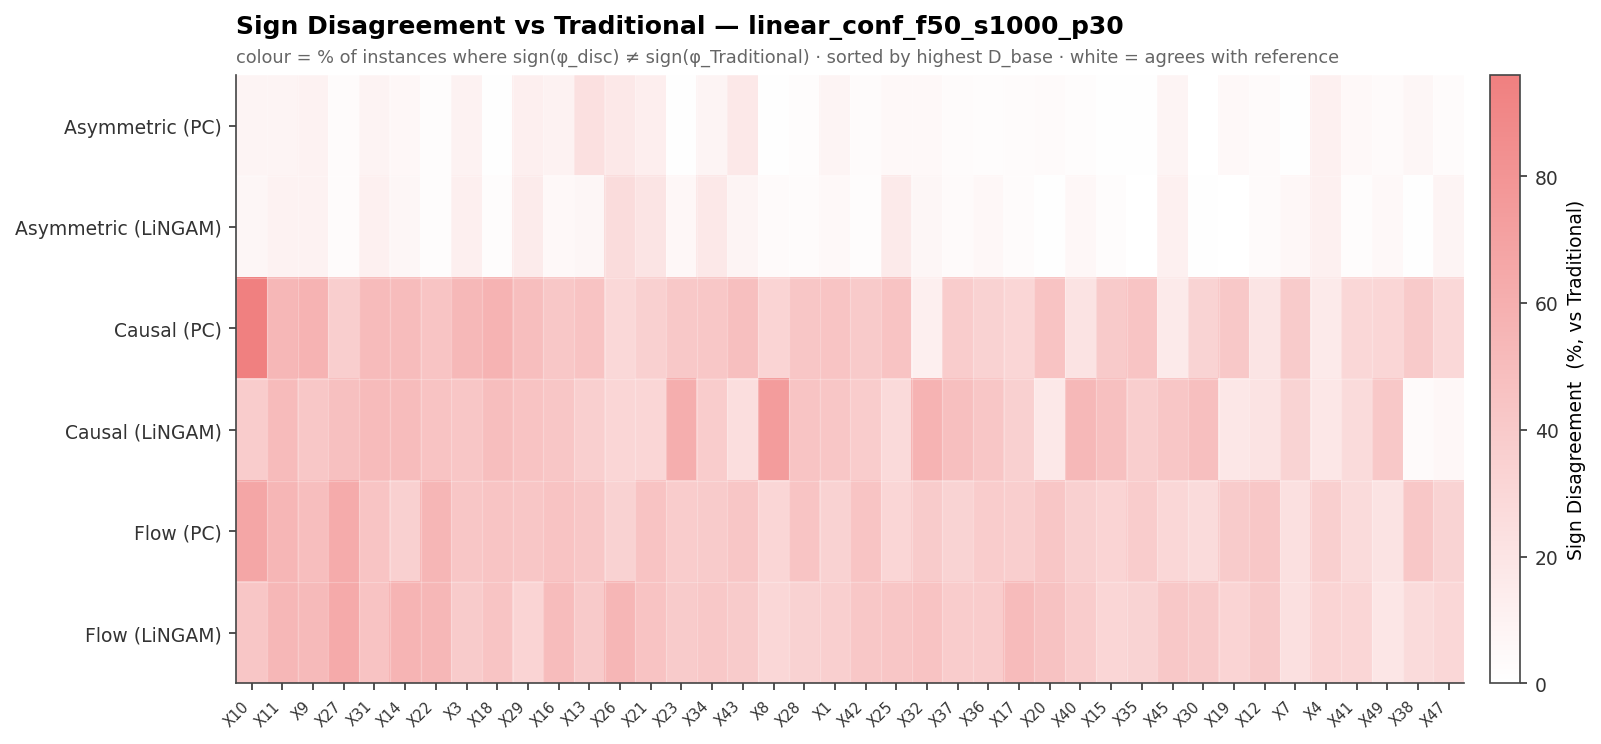
\includegraphics[width=\linewidth]{figures/sign_alignment_heatmap_traditional_linear_conf_f50_s1000_p30.png}
    \caption{Synthetic dataset (top 10 features by mean $D_{\text{base}}$). Rows are method-graph combinations; columns are features. The Asymmetric rows are near-zero throughout; Causal and Flow show elevated sign-flip rates concentrated on the same dominant features as the magnitude heatmap.}
    \label{fig:sign_trad_synth}
  \end{subfigure}
  \hfill
  \begin{subfigure}[t]{0.48\linewidth}
    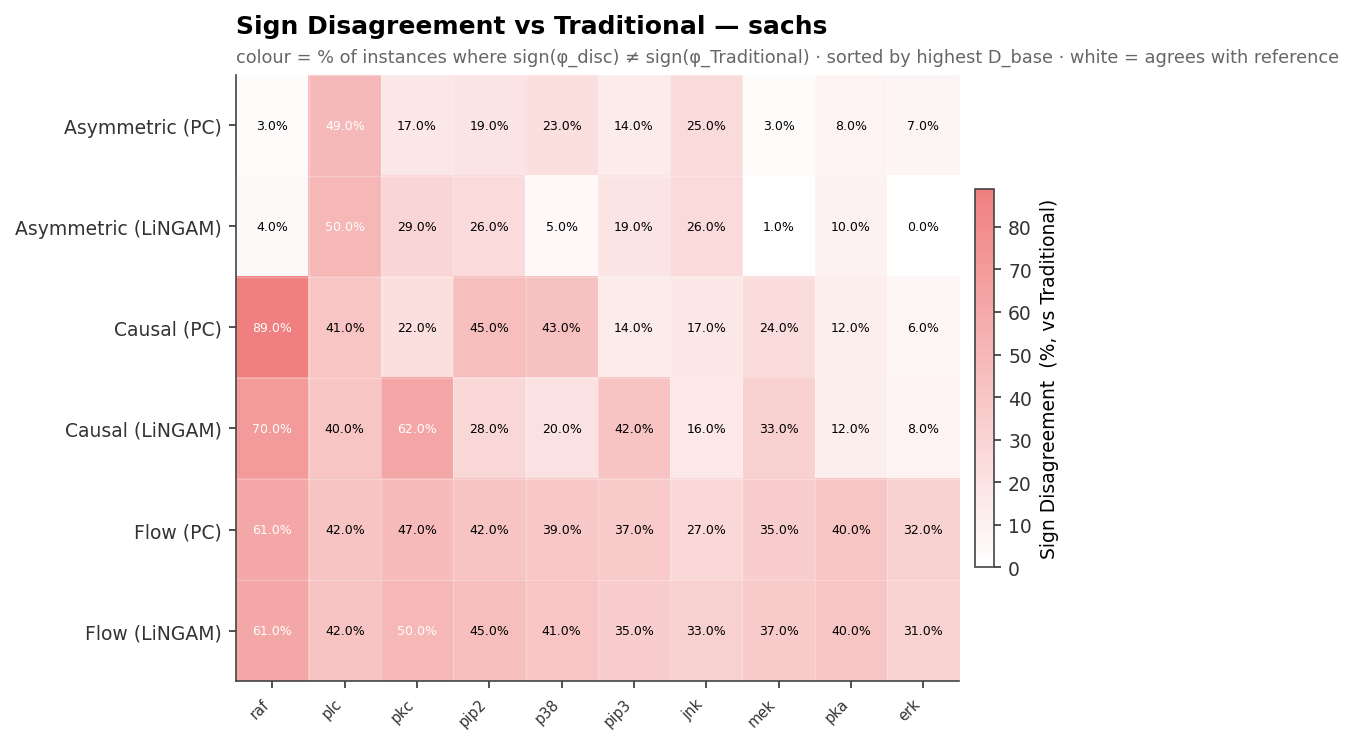
\includegraphics[width=\linewidth]{figures/sign_alignment_heatmap_traditional_sachs.png}
    \caption{Sachs dataset (top 10 features by mean $D_{\text{base}}$). Sign disagreement concentrates on raf, plc, pkc, with Causal under LiNGAM producing the highest per-feature sign-flip rate against the graph-free baseline.}
    \label{fig:sign_trad_sachs}
  \end{subfigure}
  \caption{\textbf{Feature-level Sign Disagreement $D_{\text{base}}$ vs.\ Traditional Shapley.}}
  \label{fig:sign_trad}
\end{figure}

The method hierarchy is the same: Asymmetric rows remain uniformly pale, except for plc, which has too many parents in the discovered graph and is therefore highly restricted in the causal ordering, while Causal and Flow concentrate their sign flips on the dominant features, confirming that magnitude inflation and sign inversion co-locate on the same nodes.

\subsubsection{Asymmetric Shapley: High Robustness to Graph Injection}

Asymmetric Shapley achieves the closest agreement with the Traditional Shapley baseline across both datasets. On the synthetic track, $D_{\text{base}} = 5.08\%$ (PC) and $5.76\%$ (LiNGAM), with $\Delta M_{\text{base}} = 0.68\%$ and $0.86\%$ respectively: fewer than 6\% of attribution signs change and the magnitude shift is under 1\% of $\hat{\sigma}$. On Sachs the deviation $D_{\text{base}}$ triples (16.80--17.00\%), also not bad if compared with the behaviour of Causal Shapley and Shapley Flow on synthetic dataset, and $\Delta M_{\text{base}}$ 4.41--5.08\% of $\hat{\sigma}$, the larger numbers reflecting the compact 10-node network where each ordering constraint binds a larger share of the graph. In both cases ASV remains the method that perturbs the baseline least.

The reason is structural: ASV changes only the permutation space and leaves the observational value function untouched, so its deviation from Traditional depends solely on how many orderings the graph forbids. The discovered graphs forbid very few, none of the PC or LiNGAM graphs form long directed chains, so most feature pairs stay order-free and the admissible permutations remain close to the full $N!$ set. The averaging therefore runs over almost the same orderings as Traditional and the attributions barely move, least of all on the larger, sparser synthetic graph.

The higher $D_{\text{base}}$ on Sachs ($\sim$17\% vs $\sim$5\% synthetic) could be related to its skewed importance profile, with attribution mass concentrated in a few proteins and a long tail of near-zero values, even a small magnitude shift easily pushes a fragile attribution across zero and registers as a sign flip.

\subsubsection{Causal Shapley: Intermediate Deviation with Interventional Redistribution}

Causal Shapley diverges from Traditional Shapley far more than Asymmetric with a general sign disagreement $D_{\text{base}}$ around 33.92--35.30\% and $\Delta M_{\text{base}}$ around 5.84--6.39\% on synthetic, with $D_{\text{base}}$ 31.30--33.10\% and $\Delta M_{\text{base}}$ 7.83--9.31\% of $\hat{\sigma}$ on Sachs. Replacing observational marginalization with do-distributions redistributes credit based on the discovered graph, changing the sign of roughly a third of all attributions.

A notable pattern across both datasets is that the features with the highest sign-flip rates are not the ones with the largest magnitude changes. Features such as X10 (synthetic) and raf (Sachs) do not rank among the top features by $\Delta M_{\text{base}}$, they fall outside the highest-perturbation columns in the heatmap, yet they show the highest sign disagreement. The reason is that their Traditional Shapley values sit close to zero; a small interventional redistribution is sufficient to push the attribution across zero and invert its sign. Larger-magnitude features absorb the same redistribution without crossing zero. The specific features that best exemplify the source-versus-intermediate credit shift are examined in Section~\ref{sec:cases}.

\subsubsection{Shapley Flow: High Deviation with Sign Instability}

Shapley Flow shows the highest Sign Disagreement on the synthetic dataset ($D_{\text{base}} = 36.58$--$37.68\%$) and the largest magnitude deviation overall, reaching $\Delta M_{\text{base}} = 14.17\%$ of $\hat{\sigma}$ on Sachs under LiNGAM. The two move together: re-routing credit along edges produces large magnitude shifts, and the larger the magnitude shift the more often it is large enough to carry an attribution across zero and invert its sign. Flow's high magnitude deviation is therefore the direct cause of its high sign instability.

Read per feature, the signed instance-level gap has a structural meaning for Flow: the discriminating quantity is the node's balance of incoming to outgoing edges. A node's attribution is the sum of its outgoing edge credits, so a feature with many incoming edges spends its activation propagating its parents' credit forward and tends to lose magnitude, while a feature with a high outgoing-to-incoming ratio accumulates edge credit and tends to gain it. The features that best illustrate these mechanisms, including cases where a node's edge balance flips between the two discovered graphs, are deferred to Section~\ref{sec:cases}.

\subsection{True-Graph Causal Alignment}
\label{sec:oracle_align}

The oracle-alignment analysis measures how closely each combination of structure-aware Shapley method and discovered graph recovers the attributions that would be obtained with the oracle graph as input. On the synthetic track the oracle is the True DAG; on Sachs it is the consensus reference DAG, which plays the same role. Tables~\ref{tab:oracle_synth}--\ref{tab:oracle_sachs} report $\Delta M_{\text{oracle}}$ and $D_{\text{oracle}}$ for each track, and Figures~\ref{fig:scatter_oracle} place every configuration on the magnitude axis ($\Delta M_{\text{oracle}}$) against the sign axis ($D_{\text{oracle}}$), where the lower-left corner marks the closest recovery of the oracle attributions. A clear pattern emerges across both tracks, the algorithm that achieves better causal discovery accuracy consistently produces smaller oracle deviation, which could sound logical, but we will see that even in noisy scenarios it have big difference. On the synthetic dataset the margin is modest---Causal Shapley under PC (F1 = 0.567) reaches $D_{\text{oracle}} = 31.60\%$ and $\Delta M_{\text{oracle}} = 5.32\%$, versus 37.46\% and 7.57\% under LiNGAM (F1 = 0.250)---yet the direction is unambiguous, with PC (the stronger discovery algorithm on this track) occupying the lower-left region of the scatter plot in every method. The effect is more striking on Sachs, where neither algorithm scores well in absolute discovery terms but LiNGAM outperforms PC (F1 = 0.326 vs.\ 0.167): Asymmetric Shapley under LiNGAM achieves $\Delta M_{\text{oracle}} = 2.84\%$ versus 9.16\% under PC, and Shapley Flow drops from 15.52\% to 8.12\% when switching from PC to LiNGAM. This demonstrates that imperfect graph discovery does not disqualify structure-aware methods: even with a noisy discovered graph, the better of the two candidate algorithms closes a substantial portion of the gap to the oracle. Among the three methods, Asymmetric Shapley is the least penalised by graph misspecification, at least in the magnitude divergence, its oracle deviation remains low regardless of which discovered graph is supplied, making it the safest choice when discovery quality cannot be guaranteed.

\begin{figure}[H]
  \centering
  \begin{subfigure}[t]{0.48\linewidth}
    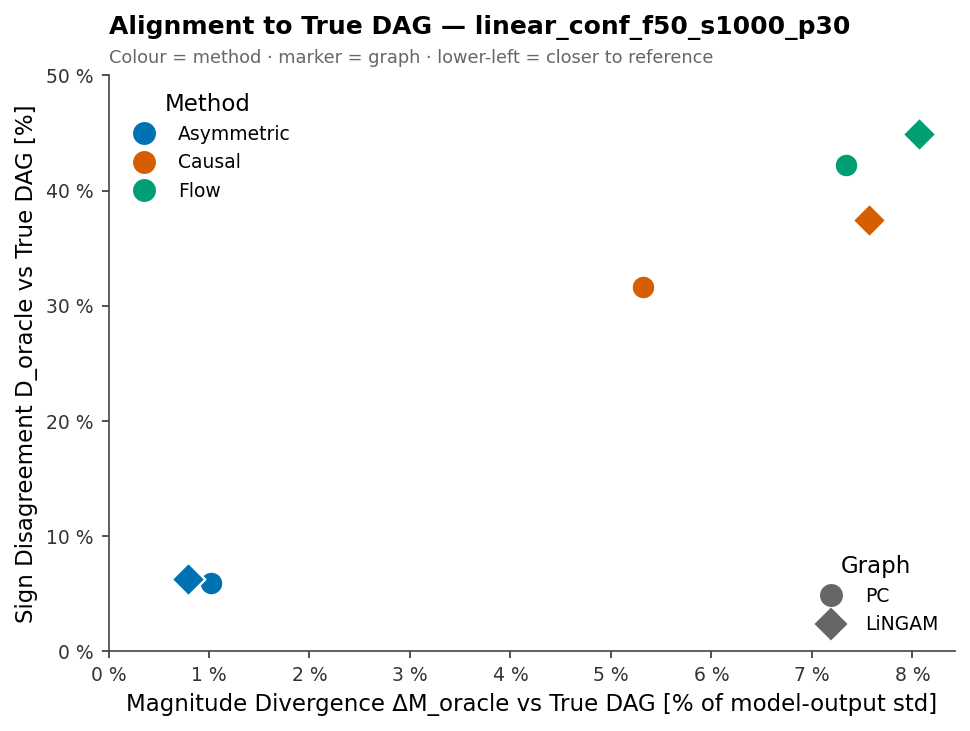
\includegraphics[width=\linewidth]{figures/tga_sa_scatter_true_linear_conf_f50_s1000_p30.png}
    \caption{Synthetic dataset. Asymmetric Shapley sits in the lower-left corner under both graphs, recovering the oracle attributions almost exactly, while Causal and Flow sit far up and to the right.}
    \label{fig:scatter_oracle_synth}
  \end{subfigure}
  \hfill
  \begin{subfigure}[t]{0.48\linewidth}
    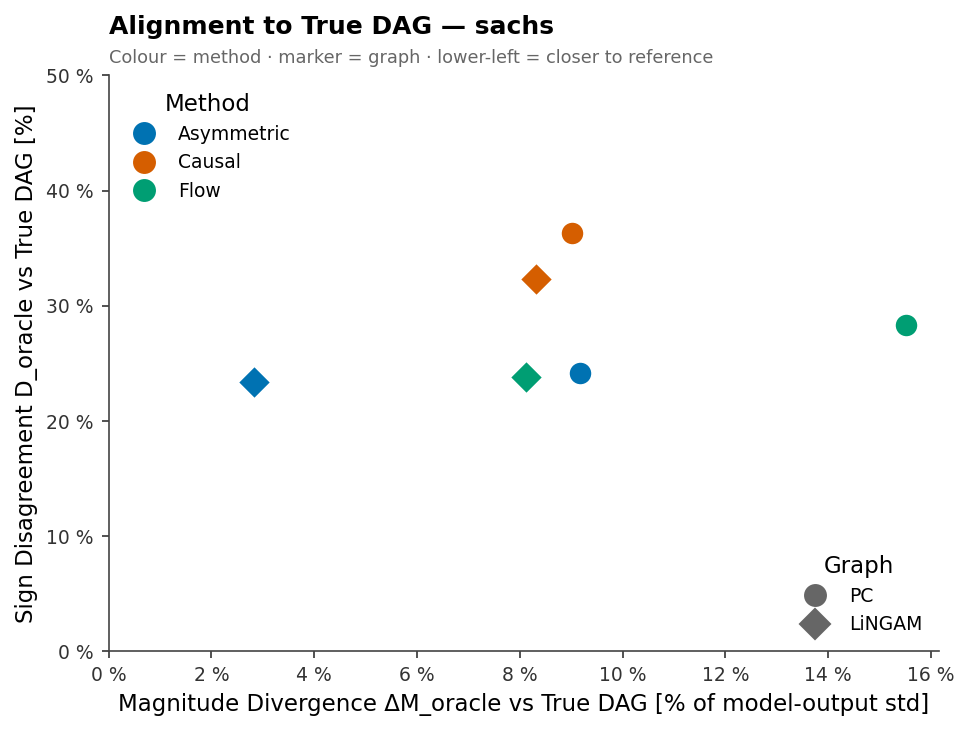
\includegraphics[width=\linewidth]{figures/tga_sa_scatter_true_sachs.png}
    \caption{Sachs dataset ($\Delta M_{\text{oracle}}$). The lower-left ordering is less clean than on the synthetic track: Asymmetric still aligns best on magnitude, but the sign axis compresses the three methods together and the PC/LiNGAM markers separate widely on magnitude.}
    \label{fig:scatter_oracle_sachs}
  \end{subfigure}
  \caption{\textbf{Magnitude versus sign deviation from the oracle DAG.}}
  \label{fig:scatter_oracle}
\end{figure}

\begin{table}[H]
  \centering
  \caption{\textbf{Oracle Alignment -- Linear-Conf Synthetic Dataset.} $D_{\text{oracle}}$ and $\Delta M_{\text{oracle}}$ in \% of $\hat{\sigma}$.}
  \label{tab:oracle_synth}
  \begin{tabular}{llrr}
    \toprule
    \textbf{Method} & \textbf{Graph} & $D_{\text{oracle}}$ & $\Delta M_{\text{oracle}}$ \\
    \midrule
    Asymmetric & PC     & 5.88\%  & 1.02\% \\
    Asymmetric & LiNGAM & 6.30\%  & 0.79\% \\
    Causal     & PC     & 31.60\% & 5.32\% \\
    Causal     & LiNGAM & 37.46\% & 7.57\% \\
    Flow       & PC     & 42.26\% & 7.34\% \\
    Flow       & LiNGAM & 44.91\% & 8.06\% \\
    \bottomrule
  \end{tabular}
\end{table}

\begin{table}[H]
  \centering
  \caption{\textbf{Oracle Alignment -- Sachs Cell Signaling Dataset (oracle = consensus DAG).} $D_{\text{oracle}}$ and $\Delta M_{\text{oracle}}$ in \% of $\hat{\sigma}$.}
  \label{tab:oracle_sachs}
  \begin{tabular}{llrr}
    \toprule
    \textbf{Method} & \textbf{Graph} & $D_{\text{oracle}}$ & $\Delta M_{\text{oracle}}$ \\
    \midrule
    Asymmetric & PC     & 24.26\% & 9.16\%  \\
    Asymmetric & LiNGAM & 23.40\% & 2.84\%  \\
    Causal     & PC     & 36.30\% & 9.01\%  \\
    Causal     & LiNGAM & 32.30\% & 8.31\%  \\
    Flow       & PC     & 28.36\% & 15.52\% \\
    Flow       & LiNGAM & 23.81\% & 8.12\%  \\
    \bottomrule
  \end{tabular}
\end{table}

\begin{figure}[H]
  \centering
  \begin{subfigure}[t]{0.48\linewidth}
    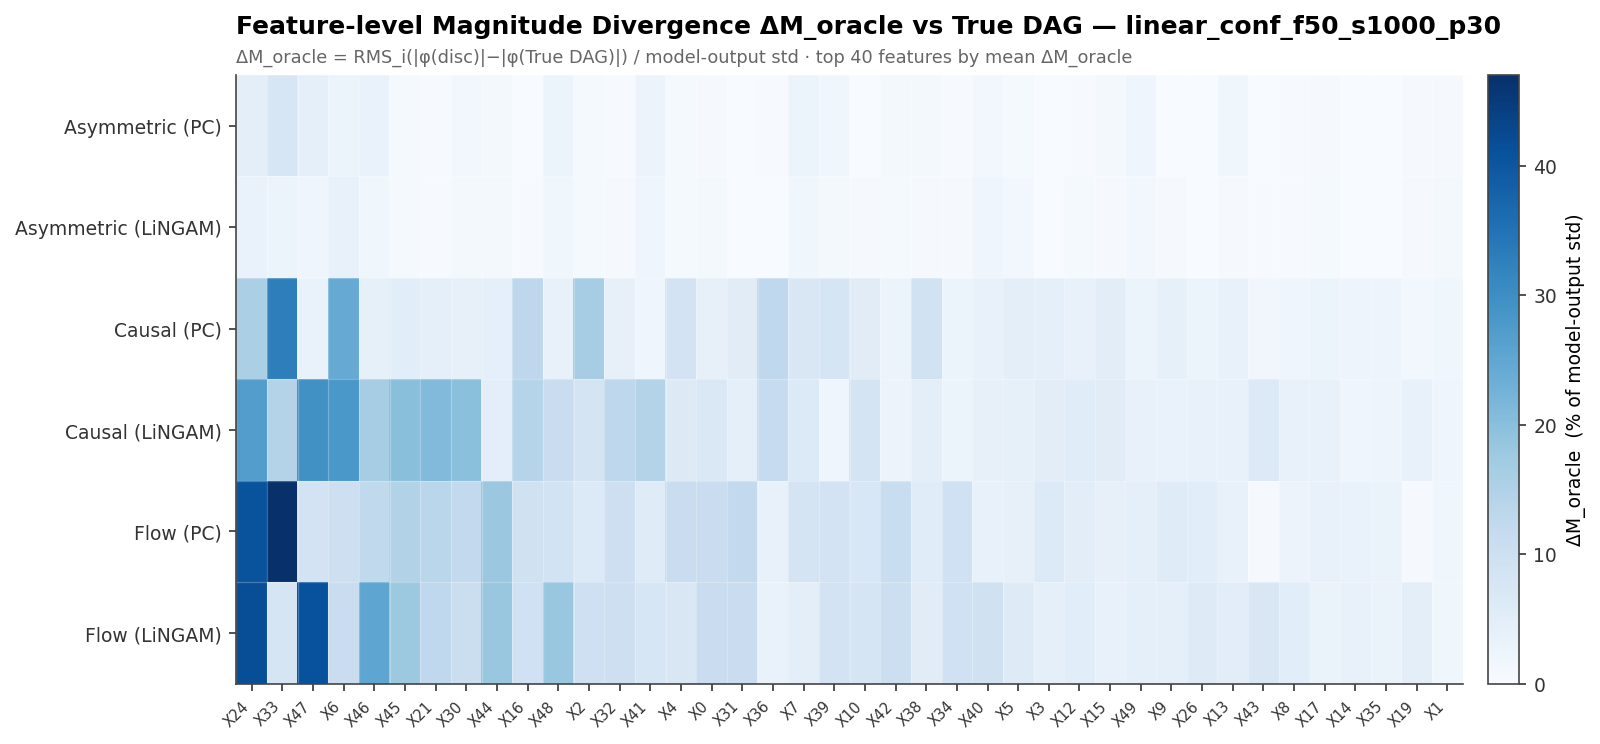
\includegraphics[width=\linewidth]{figures/tga_heatmap_true_linear_conf_f50_s1000_p30.png}
    \caption{Synthetic dataset (top 10 features by mean $\Delta M_{\text{oracle}}$). Asymmetric rows are near-zero; Causal and Flow concentrate their oracle deviations on X24, X33, X47 and X6.}
    \label{fig:heatmap_oracle_synth}
  \end{subfigure}
  \hfill
  \begin{subfigure}[t]{0.48\linewidth}
    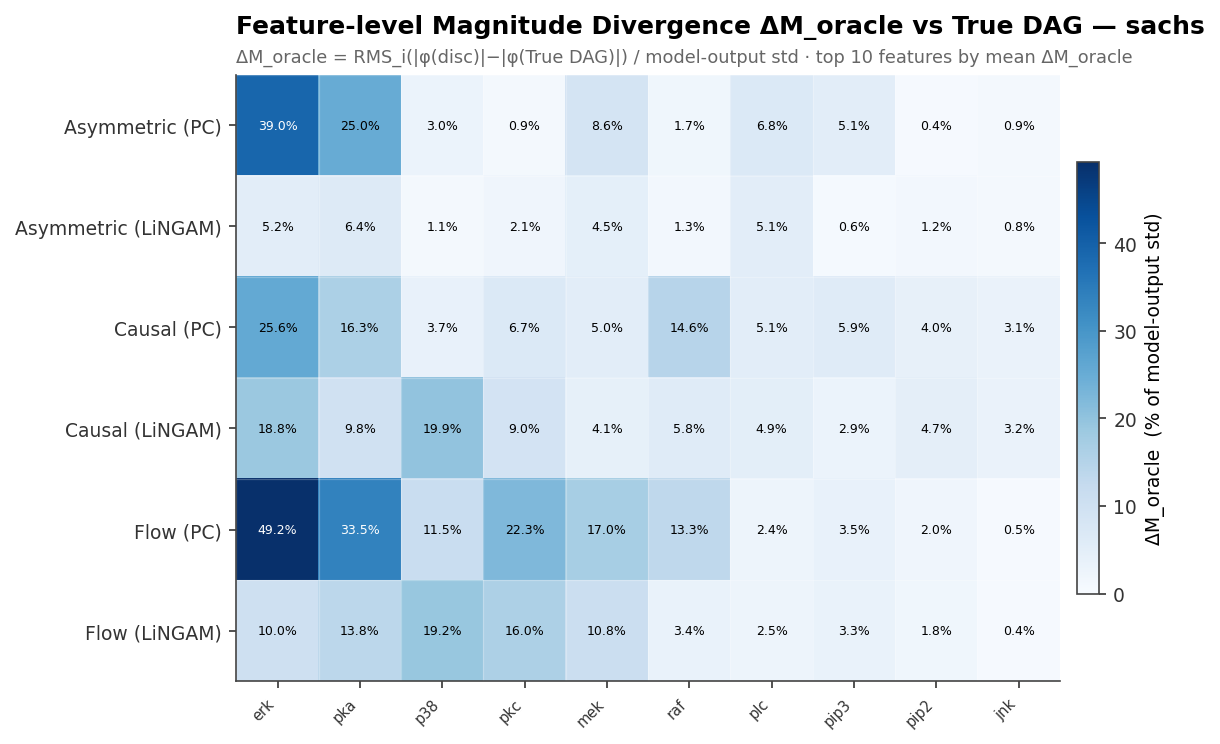
\includegraphics[width=\linewidth]{figures/tga_heatmap_true_sachs.png}
    \caption{Sachs dataset (top 10 features by mean $\Delta M_{\text{oracle}}$). Flow under PC produces the largest single deviation on erk (49.2\% of $\hat{\sigma}$), the protein PC isolates by deleting its parent links.}
    \label{fig:heatmap_oracle_sachs}
  \end{subfigure}
  \caption{\textbf{Feature-level Magnitude Divergence $\Delta M_{\text{oracle}}$ vs.\ the oracle DAG.}}
  \label{fig:heatmap_oracle}
\end{figure}

The feature-level breakdown of these oracle deviations confirms that Asymmetric rows stay pale across nearly all features while Causal and Flow darken on the dominant ones. Two details stand out: on synthetic, Flow under PC produces the single darkest cell on X33, the feature isolated as a spurious root by PC's edge reversals. On Sachs, Flow under PC reaches a feature-level $\Delta M_{\text{oracle}}$ of 49.2\% of $\hat{\sigma}$ on erk, concentrating the worst oracle deviation on a single mis-oriented node.

\begin{figure}[H]
  \centering
  \begin{subfigure}[t]{0.48\linewidth}
    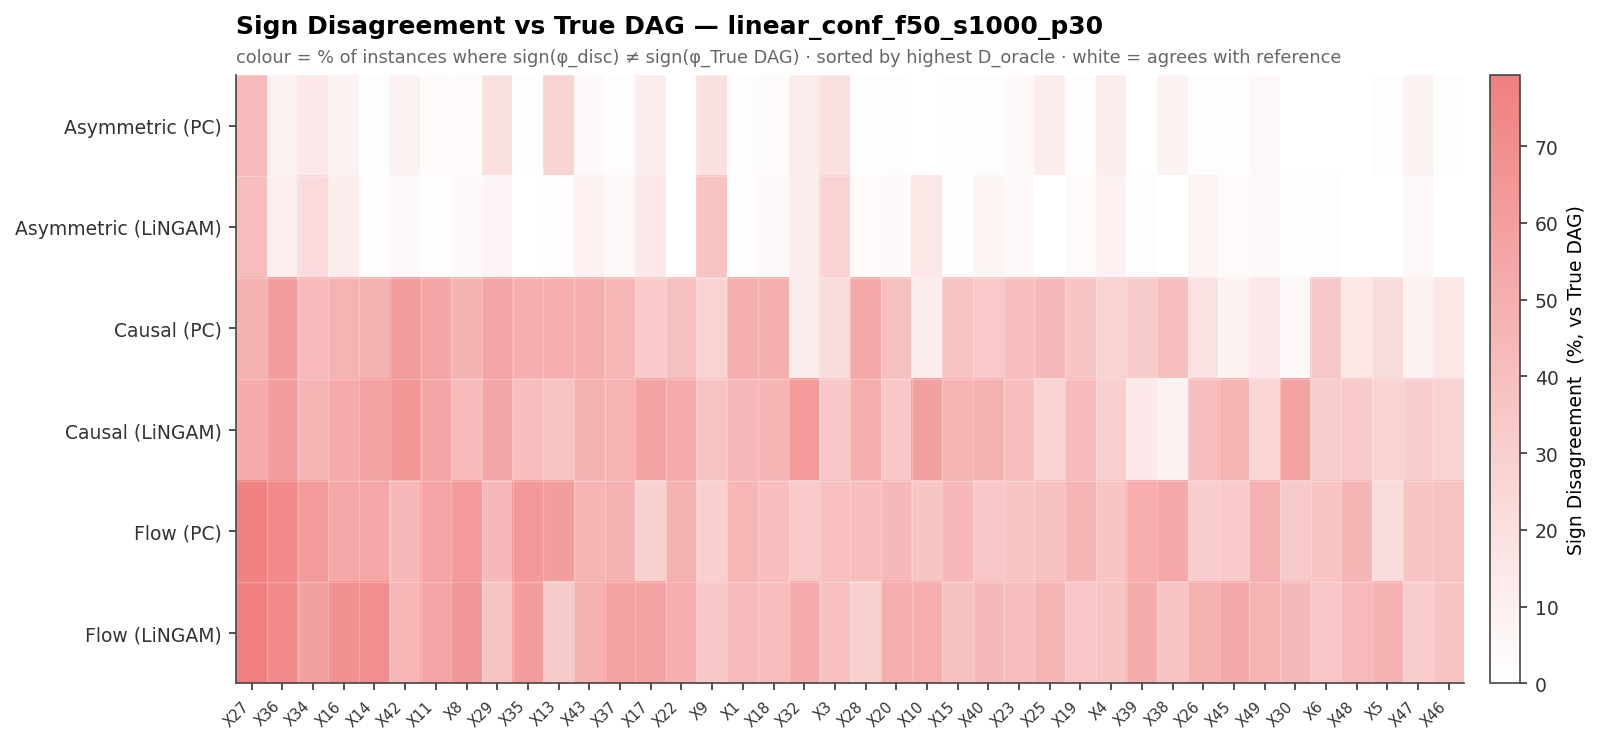
\includegraphics[width=\linewidth]{figures/sign_alignment_heatmap_true_linear_conf_f50_s1000_p30.png}
    \caption{Synthetic dataset (top 10 features by mean $D_{\text{oracle}}$). Asymmetric rows are near-zero; Causal and Flow show the highest sign disagreement on X24, X33, X47 and X6, the same dominant features that carry the oracle magnitude deviations.}
    \label{fig:sign_oracle_synth}
  \end{subfigure}
  \hfill
  \begin{subfigure}[t]{0.48\linewidth}
    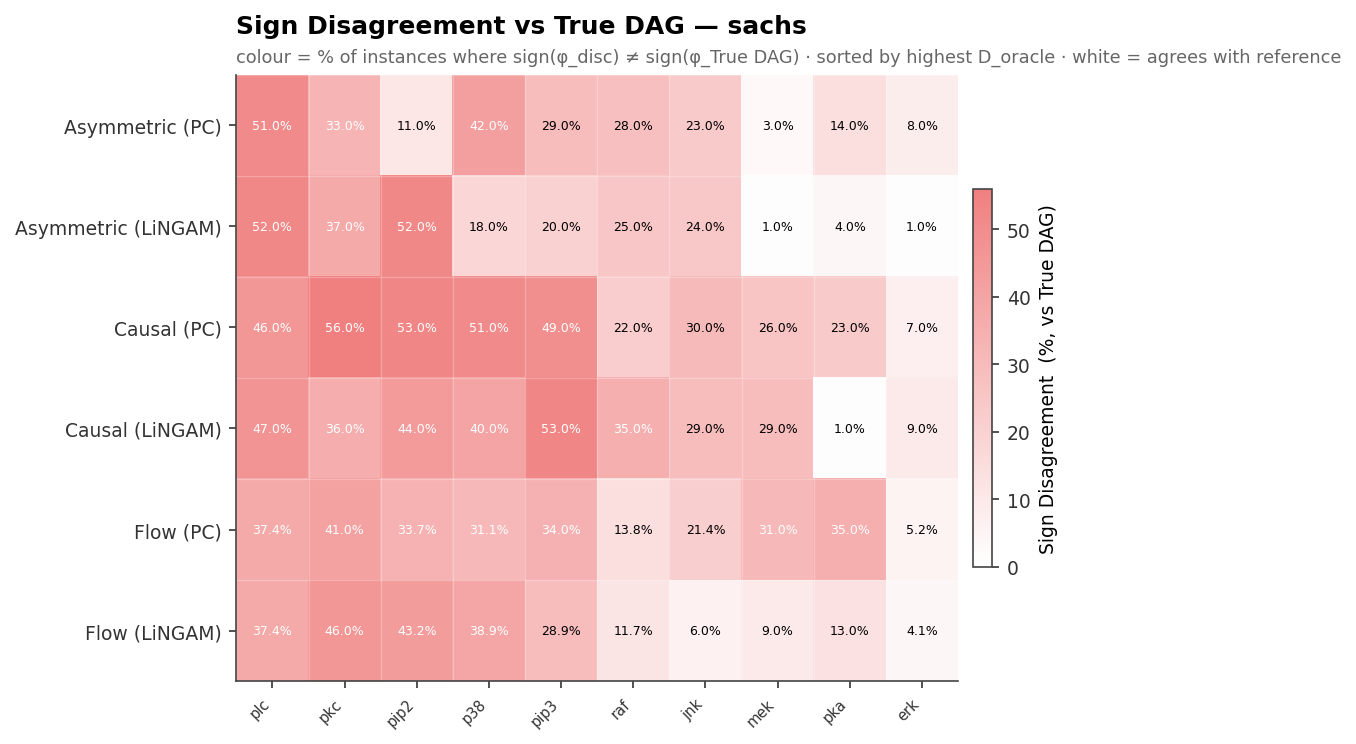
\includegraphics[width=\linewidth]{figures/sign_alignment_heatmap_true_sachs.png}
    \caption{Sachs dataset (top 10 features by mean $D_{\text{oracle}}$). Sign disagreement concentrates on erk and pka; Flow under PC produces the highest per-feature oracle sign-flip rate on erk, consistent with its largest magnitude deviation on that protein.}
    \label{fig:sign_oracle_sachs}
  \end{subfigure}
  \caption{\textbf{Feature-level Sign Disagreement $D_{\text{oracle}}$ vs.\ the oracle DAG.}}
  \label{fig:sign_oracle}
\end{figure}

The directional picture mirrors the magnitude one: Asymmetric Shapley preserves oracle attribution signs almost perfectly, while Causal and Flow flip the sign of the dominant features with the same ranking seen in the magnitude heatmaps.

\subsubsection{Asymmetric Shapley: Near-Perfect Oracle Fidelity}

On the synthetic dataset ASV achieves the highest alignment with the True DAG oracle: $D_{\text{oracle}} = 5.88\%$ (PC) and $6.30\%$ (LiNGAM), with $\Delta M_{\text{oracle}} = 1.02\%$ and $0.79\%$ of $\hat{\sigma}$ respectively. Despite LiNGAM injecting 81 false-positive edges, the additional ordering constraints introduced by these edges minimally affect the attribution magnitudes. In a 50-node sparse system, the true and discovered graphs share most of their valid topological orderings, producing nearly identical attributions regardless of graph source.

On Sachs the picture is the same in relative terms but coarser in absolute terms: ASV again has the lowest sign disagreement ($D_{\text{oracle}} = 23.40$--$24.26\%$) and the lowest magnitude deviation, with LiNGAM in particular reaching $\Delta M_{\text{oracle}} = 2.84\%$ of $\hat{\sigma}$ against the consensus oracle, the closest oracle recovery of any configuration on the real track. The larger sign-disagreement floor ($\sim$24\%, versus $\sim$6\% on synthetic) reflects the compact 10-node network, where each discovery error constrains a larger fraction of the available orderings.

Notably, graph quality plays a different role depending on the axis. On the sign side, the quality of the discovered graph does not give ASV a clear advantage: the distributions of instance-level gaps are centred close to zero with high variance under both PC and LiNGAM, with no feature showing a systematic tendency to align with or oppose the True DAG attributions, and the $D_{\text{oracle}}$ values are essentially tied between the two graphs on both datasets. On the magnitude side, however, the better graph does help: on Sachs the more accurate LiNGAM graph (F1 = 0.326 vs.\ PC's F1 = 0.167) achieves $\Delta M_{\text{oracle}} = 2.84\%$ against 9.16\% for PC, a threefold reduction. Because ASV's averaging is insensitive to all but the orderings a graph forbids, and the discovered graphs forbid few, directional recovery is stable regardless of graph quality, but the smaller set of forbidden orderings under the more accurate graph does reduce the magnitude perturbation.

\subsubsection{Causal and Flow: Compounding Error Under Imprecise Graphs}

CSV and Shapley Flow show substantial vulnerability to graph prior distortion. For CSV, LiNGAM's 81 false-positive edges inject spurious parent relationships into the interventional conditioning procedure. Each false parent link causes CSV to compute post-interventional distributions that do not correspond to any real causal mechanism, misrouting attribution credit. On synthetic this yields $D_{\text{oracle}} = 37.46\%$ and $\Delta M_{\text{oracle}} = 7.57\%$ of $\hat{\sigma}$ for CSV+LiNGAM; PC's more conservative graph reduces but does not eliminate the distortion ($D_{\text{oracle}} = 31.60\%$, $\Delta M_{\text{oracle}} = 5.32\%$).

Shapley Flow shows the largest sign disagreement with the oracle on synthetic: $D_{\text{oracle}} = 42.26$--$44.91\%$, meaning close to half of all attributions point in the wrong direction relative to the True DAG. PC's under-connected graph removes pathways along which credit should flow, and LiNGAM's over-connected graph creates excessive edge competition. $\Delta M_{\text{oracle}} = 7.34$--$8.06\%$ of $\hat{\sigma}$ confirms the magnitude scale is also substantially distorted in both cases.

The Sachs track qualifies this synthetic picture in two ways. First, the CSV ordering between graphs reverses: CSV+LiNGAM ($D_{\text{oracle}} = 32.30\%$) aligns slightly better with the consensus oracle than CSV+PC (36.30\%), consistent with LiNGAM being the stronger discovery algorithm on the real non-Gaussian data. Second, Flow is markedly less sign-unstable on Sachs ($D_{\text{oracle}} = 23.81$--$28.36\%$) than on synthetic, although it still carries the largest magnitude deviations ($\Delta M_{\text{oracle}}$ up to 15.52\% of $\hat{\sigma}$ for Flow+PC). The contrast indicates that Flow's extreme synthetic sign instability is partly a property of the dense, heavily mis-oriented synthetic graphs rather than an invariant of the method.

\subsection{Discovery Algorithm Sensitivity Analysis}
\label{sec:disc_analysis}

This final comparison answers a practical question: if a practitioner runs two discovery algorithms on the same data and feeds each graph into the same Shapley method, how much do the explanations change? The answer depends heavily on the method, and the effect is larger on the sign of attributions than on their magnitude. Asymmetric Shapley consistently shows the lowest sensitivity, keeping both $\Delta M_{\text{disc}}$ and $D_{\text{disc}}$ well below its counterparts on both datasets. The gap is most visible on the real data: Flow's magnitude divergence between the two graphs ($\Delta M_{\text{disc}} = 14.92\%$ of $\hat{\sigma}$) is nearly double Asymmetric's (8.46\%), meaning that choosing Shapley Flow instead of Asymmetric makes the explanation twice as sensitive in magnitude depending solely on which discovery algorithm was run. On the sign axis, choosing between Causal Shapley and Asymmetric Shapley for the Sachs dataset determines whether switching from one discovered graph to the other flips 31.80\% or 18.60\% of attribution signs---Causal disagrees with itself across graphs at almost double the rate of Asymmetric.

Figures~\ref{fig:scatter_disc} plot the two quantities against each other; the lower-left corner marks a method whose attributions are stable regardless of which discovery algorithm was used. Tables~\ref{tab:disc_synth}--\ref{tab:disc_sachs} quantify how much the choice between PC and LiNGAM affects the final attributions for each Shapley method.

\begin{figure}[H]
  \centering
  \begin{subfigure}[t]{0.48\linewidth}
    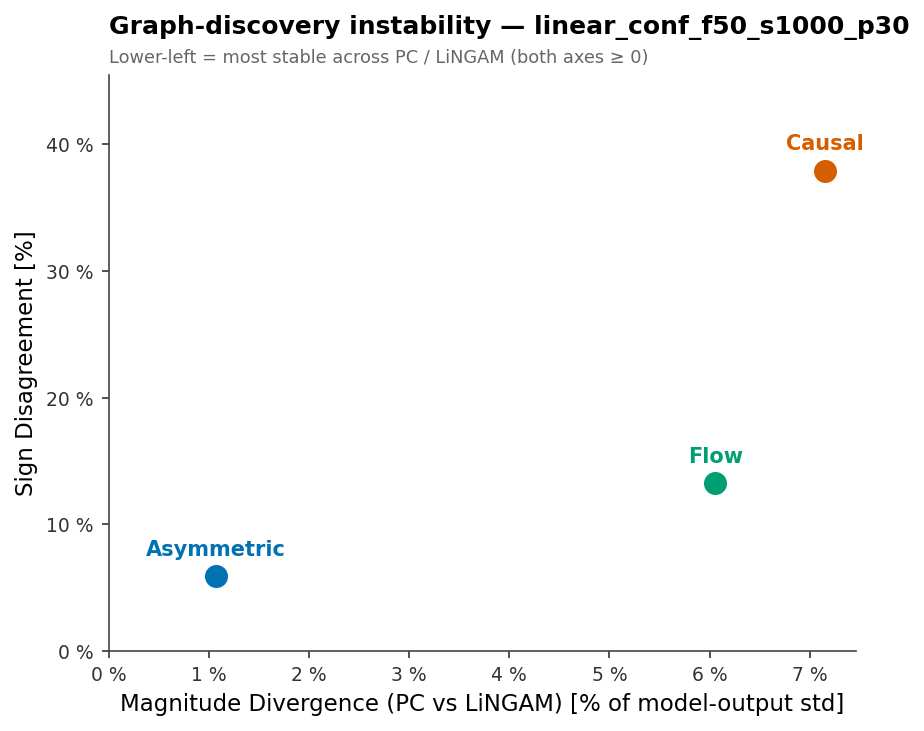
\includegraphics[width=\linewidth]{figures/gss_sss_scatter_linear_conf_f50_s1000_p30.png}
    \caption{Synthetic dataset. Asymmetric sits in the lower-left (stable on both axes), Causal in the upper-right (unstable on both), and Flow in between, magnitude-sensitive but comparatively sign-stable.}
    \label{fig:scatter_disc_synth}
  \end{subfigure}
  \hfill
  \begin{subfigure}[t]{0.48\linewidth}
    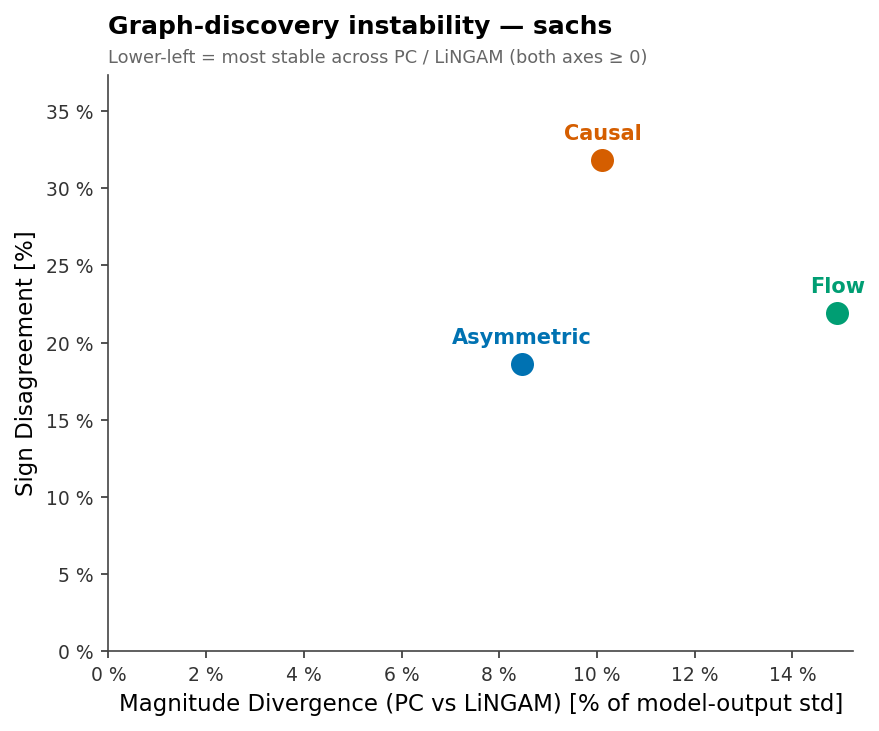
\includegraphics[width=\linewidth]{figures/gss_sss_scatter_sachs.png}
    \caption{Sachs dataset ($\Delta M_{\text{disc}}$). The same ordering holds, with both axes wider than on synthetic; Causal remains the most sign-unstable while Flow carries the largest magnitude difference between graphs.}
    \label{fig:scatter_disc_sachs}
  \end{subfigure}
  \caption{\textbf{Graph-discovery instability (PC vs.\ LiNGAM).}}
  \label{fig:scatter_disc}
\end{figure}

\begin{table}[H]
  \centering
  \begin{minipage}[t]{0.48\linewidth}
    \centering
    \caption{\textbf{PC vs.\ LiNGAM Sensitivity -- Synthetic.}}
    \label{tab:disc_synth}
    \begin{tabular}{lrr}
      \toprule
      \textbf{Method} & $\Delta M_{\text{disc}}$ & $D_{\text{disc}}$ \\
      \midrule
      Asymmetric & 1.07\%  & 5.93\%  \\
      Causal     & 7.15\%  & 37.94\% \\
      Flow       & 6.06\%  & 13.27\% \\
      \bottomrule
    \end{tabular}
  \end{minipage}
  \hfill
  \begin{minipage}[t]{0.48\linewidth}
    \centering
    \caption{\textbf{PC vs.\ LiNGAM Sensitivity -- Sachs.}}
    \label{tab:disc_sachs}
    \begin{tabular}{lrr}
      \toprule
      \textbf{Method} & $\Delta M_{\text{disc}}$ & $D_{\text{disc}}$ \\
      \midrule
      Asymmetric & 8.46\%  & 18.60\% \\
      Causal     & 10.11\% & 31.80\% \\
      Flow       & 14.92\% & 21.88\% \\
      \bottomrule
    \end{tabular}
  \end{minipage}
\end{table}

\begin{figure}[H]
  \centering
  \begin{subfigure}[t]{0.48\linewidth}
    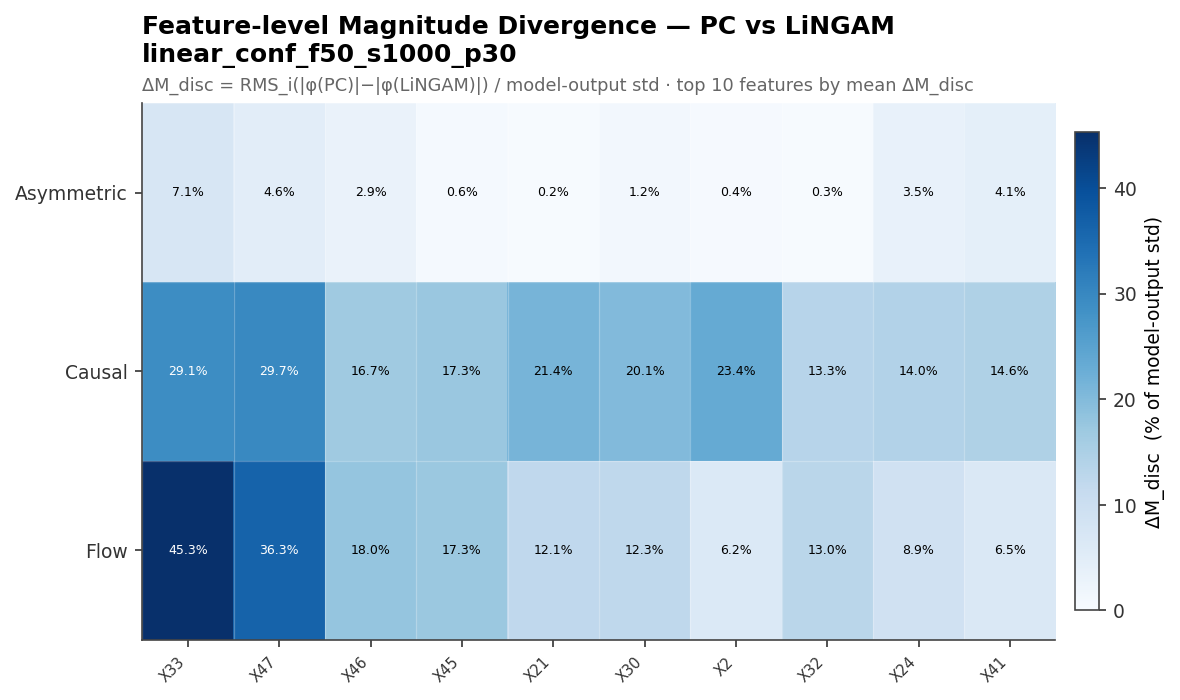
\includegraphics[width=\linewidth]{figures/gss_heatmap_linear_conf_f50_s1000_p30.png}
    \caption{Synthetic dataset (top 10 features by mean $\Delta M_{\text{disc}}$). The Asymmetric row is near-zero; Causal and Flow concentrate their PC-vs-LiNGAM magnitude differences on X33 and X47, with Flow producing the single darkest cell on X33.}
    \label{fig:gss_synth}
  \end{subfigure}
  \hfill
  \begin{subfigure}[t]{0.48\linewidth}
    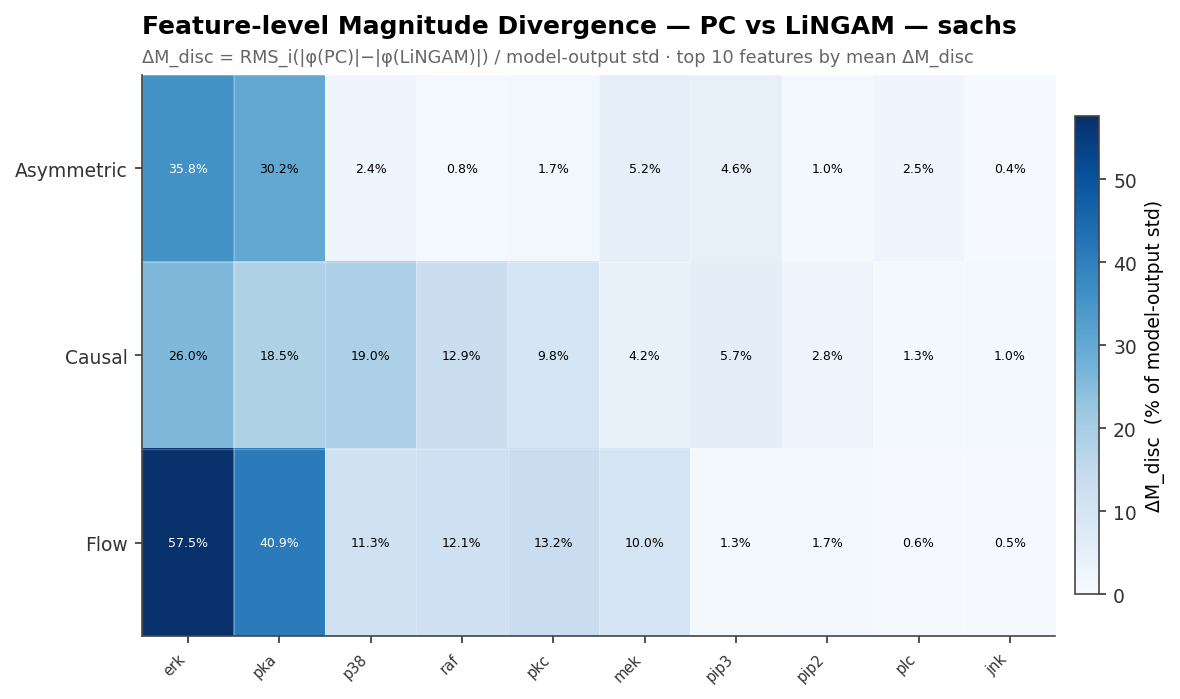
\includegraphics[width=\linewidth]{figures/gss_heatmap_sachs.png}
    \caption{Sachs dataset (top 10 features by mean $\Delta M_{\text{disc}}$). The sensitivity concentrates on erk and pka across all three methods, with Flow reaching a feature-level $\Delta M_{\text{disc}}$ of 57.5\% of $\hat{\sigma}$ on erk.}
    \label{fig:gss_sachs}
  \end{subfigure}
  \caption{\textbf{Feature-level cross-discovery Magnitude Divergence $\Delta M_{\text{disc}}$ (PC vs.\ LiNGAM).}}
  \label{fig:gss}
\end{figure}

The feature-level breakdown of $\Delta M_{\text{disc}}$ reveals which features are most sensitive to the choice of discovered DAG for each Shapley method. On the synthetic dataset, Asymmetric Shapley remains near-zero across all features, its per-feature $\Delta M_{\text{disc}}$ stays well within a single percentage point of $\hat{\sigma}$. The picture shifts on Sachs: even Asymmetric shows elevated sensitivity on erk and pka, driven by the large structural differences between the PC and LiNGAM graphs on those two proteins rather than by a weakness of the method itself.

\begin{figure}[H]
  \centering
  \begin{subfigure}[t]{0.48\linewidth}
    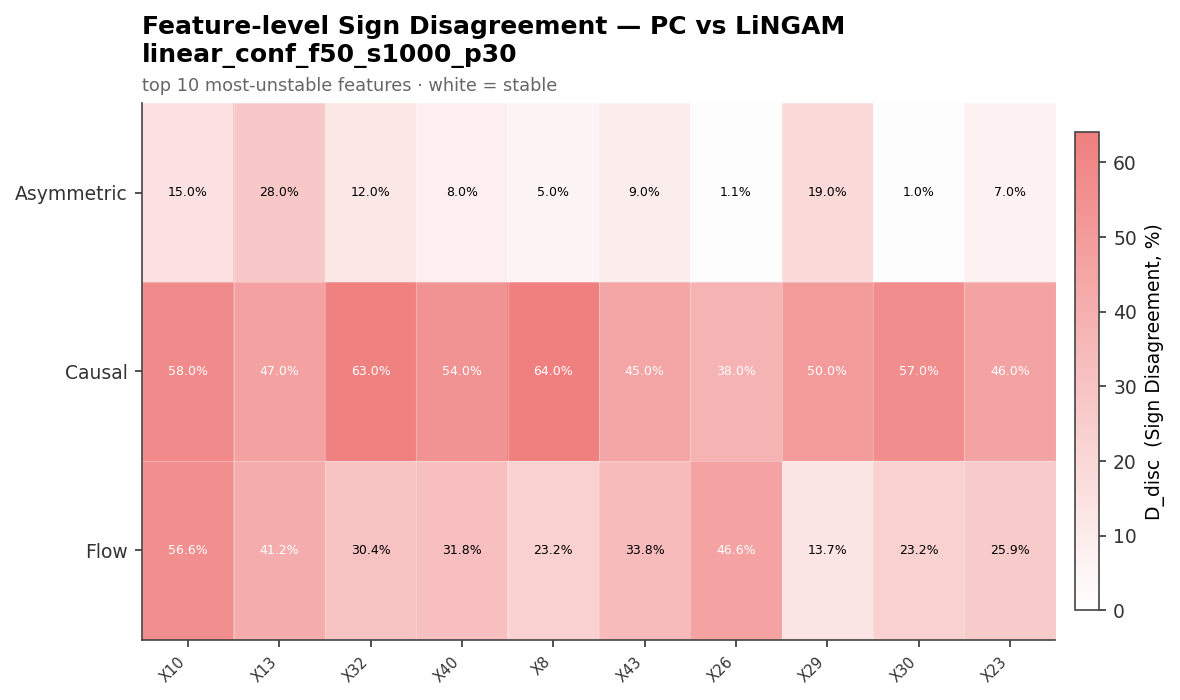
\includegraphics[width=\linewidth]{figures/sss_heatmap_linear_conf_f50_s1000_p30.png}
    \caption{Synthetic dataset (top 10 features by mean $D_{\text{disc}}$). The Asymmetric row is clearly low; Causal shows the highest sign instability concentrated on X10 and X32, while Flow's sign instability is moderate compared to its magnitude sensitivity.}
    \label{fig:sss_synth}
  \end{subfigure}
  \hfill
  \begin{subfigure}[t]{0.48\linewidth}
    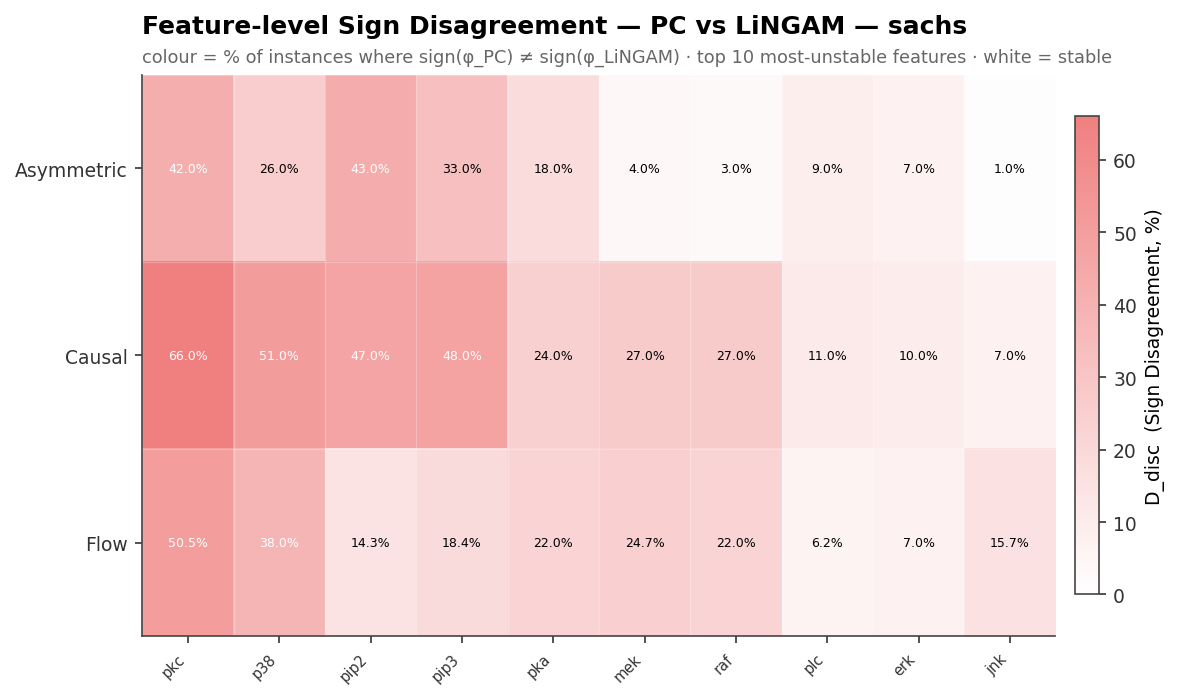
\includegraphics[width=\linewidth]{figures/sss_heatmap_sachs.png}
    \caption{Sachs dataset (top 10 features by mean $D_{\text{disc}}$). Sign instability concentrates on pkc and p38; Causal Shapley shows the broadest sign disagreement across proteins, consistent with its highest global $D_{\text{disc}}$.}
    \label{fig:sss_sachs}
  \end{subfigure}
  \caption{\textbf{Feature-level cross-discovery Sign Disagreement $D_{\text{disc}}$ (PC vs.\ LiNGAM).}}
  \label{fig:sss}
\end{figure}

Causal Shapley carries the largest cross-discovery sign instability on both tracks, reaching up to 64\% disagreement on individual features, meaning that for 64 out of 100 evaluated instances the attribution sign flips depending solely on which discovery algorithm was used. This concentrates across methods on X10 and X13 for the synthetic dataset and on pkc and p38 for Sachs, features that are examined in detail in Section~\ref{sec:cases}.

\subsubsection{Asymmetric Shapley: Minimal Sensitivity on Synthetic}

On the synthetic dataset, ASV shows the lowest sensitivity to discovery algorithm choice: $\Delta M_{\text{disc}} = 1.07\%$ of $\hat{\sigma}$, $D_{\text{disc}} = 5.93\%$. Only about 6 in 100 attribution signs differ between the PC and LiNGAM variants on average on all features. This is explained by the high-dimensional sparse setting of the synthetic dataset: both graphs leave most ordering relationships unconstrained and ASV's permutation sampling produces nearly identical attribution distributions regardless of which graph is supplied.

On the Sachs dataset, sensitivity increases substantially to $\Delta M_{\text{disc}} = 8.46\%$ of $\hat{\sigma}$ and $D_{\text{disc}} = 18.6\%$. Opposite to the synthetic dataset, the compact 10-node Sachs network means the different edge sets discovered by PC and LiNGAM impose materially different topological constraints, and these differences accumulate into visible attribution changes, especially in nodes with known influence such as erk and pka.

\subsubsection{Causal and Flow: High Sensitivity, Especially on Real Data}

CSV and Shapley Flow are substantially more sensitive to discovery algorithm choice, but in different ways. On the synthetic dataset, CSV's $\Delta M_{\text{disc}} = 7.15\%$ and Flow's $\Delta M_{\text{disc}} = 6.06\%$ of $\hat{\sigma}$ are roughly 7 and 6 times larger than ASV's. The sign axis separates the two methods: CSV's $D_{\text{disc}} = 37.94\%$ is the highest instability in the synthetic experiment, because interventional conditioning inverts attribution signs whenever the parent sets differ between graphs, which happens frequently given LiNGAM's 81 spurious edges. Flow, by contrast, is much more sign-stable on synthetic ($D_{\text{disc}} = 13.27\%$) despite its comparable magnitude sensitivity; its cross-discovery sign instability comes largely from both discovered graphs sharing many of the same orientation errors rather than diverging from each other.

On the Sachs dataset the magnitude instability escalates: CSV's $\Delta M_{\text{disc}} = 10.11\%$ and Flow's $\Delta M_{\text{disc}} = 14.92\%$ of $\hat{\sigma}$ mean that choosing LiNGAM over PC moves CSV and Flow attributions by more than a tenth of the model-output standard deviation, making the discovery algorithm a dominant source of attribution variance. The sign-disagreement rates converge somewhat (CSV $D_{\text{disc}} = 31.80\%$, Flow 21.88\%), with CSV remaining the most sign-unstable method on both tracks. The feature-level heatmaps in Figures~\ref{fig:gss}--\ref{fig:sss} show that magnitude instability is concentrated on a few nodes: on synthetic, $\Delta M_{\text{disc}}$ focuses on X33 and X47, and on Sachs almost entirely on erk and pka, the same dominant nodes that drive every other comparison in this chapter.

Across all three comparison tracks, a consistent pattern holds: magnitude divergence is driven by a handful of focal nodes, which Section~\ref{sec:cases} examines in depth. Sign divergence, by contrast, tends to spread more broadly across features, with many near-zero attributions getting pushed across the sign boundary by small magnitude shifts. In both dimensions, Asymmetric Shapley remains the lowest-risk choice when transitioning from a graph-free baseline, whether the discovered graph is noisy, unvalidated, or switches between discovery strategies.

\subsection{Granular Case Studies}
\label{sec:cases}

Three archetypal error mechanisms illustrate the micro-level behavior observed across both experimental tracks. Each is identified by tracing a large global or feature-level metric back to a specific discovery error, using the True DAG (or the Sachs consensus DAG) as the reference for what the correct local structure should have been.

\subsubsection{Out-Degree Inflation and Root Cause Overloading}

Interventional frameworks (CSV) and edge-routing models (Flow) over-inflate the attribution of any node that a discovered graph misrepresents as a high-degree root source. The clearest synthetic case is X24, a true direct parent of $Y$ with 3 incoming and 4 outgoing edges in the True DAG. Both PC and LiNGAM strip its true parents and add spurious children (Figure~\ref{fig:dag_X24}), recasting it as an apparent high out-degree source; this inflates its interventional parent set under CSV and its outgoing-edge credit under Flow, so it absorbs compounded attribution from paths that do not exist in the true graph.

\begin{figure}[H]
  \centering
  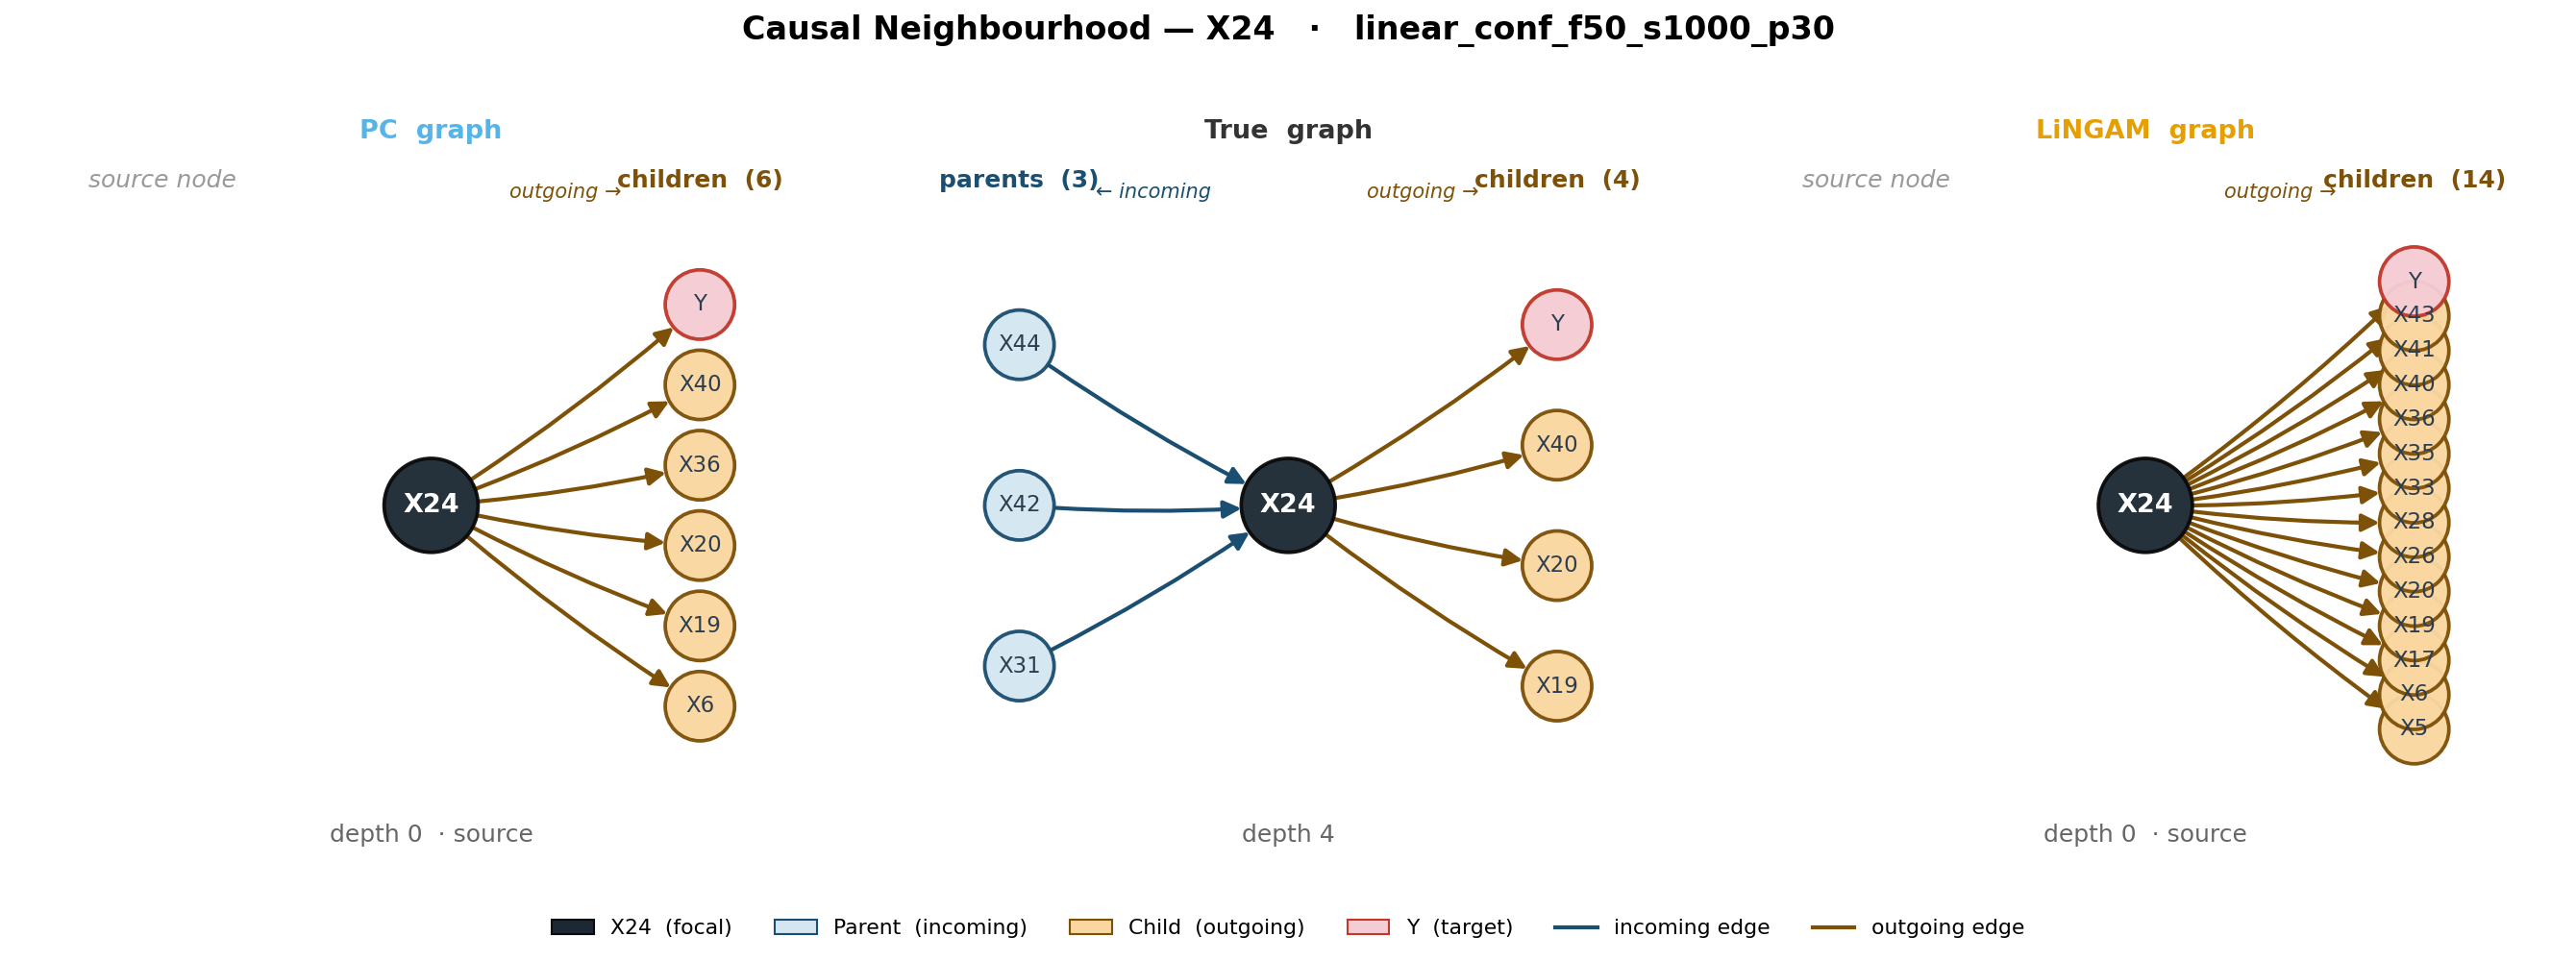
\includegraphics[width=\linewidth]{figures/dag_neighborhood_X24_linear_conf_f50_s1000_p30.png}
  \caption{\textbf{Causal neighbourhood of X24 across the PC (left), True DAG (centre), and LiNGAM (right) graphs, synthetic dataset.} Blue edges are incoming (parents), amber edges are outgoing (children). In the True DAG, X24 is a direct parent of $Y$ with 3 incoming and 4 outgoing edges. Both PC and LiNGAM strip its true incoming edges and add spurious outgoing ones (6 out-edges under PC, 14 under LiNGAM, 0 in-edges in both), recasting a mid-graph node as an apparent root source.}
  \label{fig:dag_X24}
\end{figure}

X24's feature-level $\Delta M_{\text{base}}$ against the Traditional baseline reaches 32.5\% of $\hat{\sigma}$, the highest among all features on the synthetic track. This is the signal that Section~\ref{sec:baseline} uses to flag X24 as a node worth deeper inspection. Under Traditional Shapley (no graph), X24 shows a clear, structured attribution pattern. As soon as either discovered graph is supplied, the attributions shift markedly: Flow+PC and Flow+LiNGAM both produce inflated and partially sign-flipped values relative to Flow+True, the scatter that would be obtained with the correct causal structure. This divergence is the instance-level signature of out-degree inflation: the spurious out-edges created by both discovery algorithms funnel additional credit through X24's path-accounting, moving its attributions far from the oracle. The 32.5\% $\Delta M_{\text{base}}$ is therefore not merely a global warning, it directly identifies a node whose Shapley Flow explanation should be treated as unreliable without further graph validation. More generally, a large feature-level $\Delta M_{\text{base}}$ is a practical heuristic: any feature that produces a divergence substantially above the dataset average deserves scrutiny of its discovered causal connections before its Flow attribution is used for downstream decisions.

\begin{figure}[H]
  \centering
  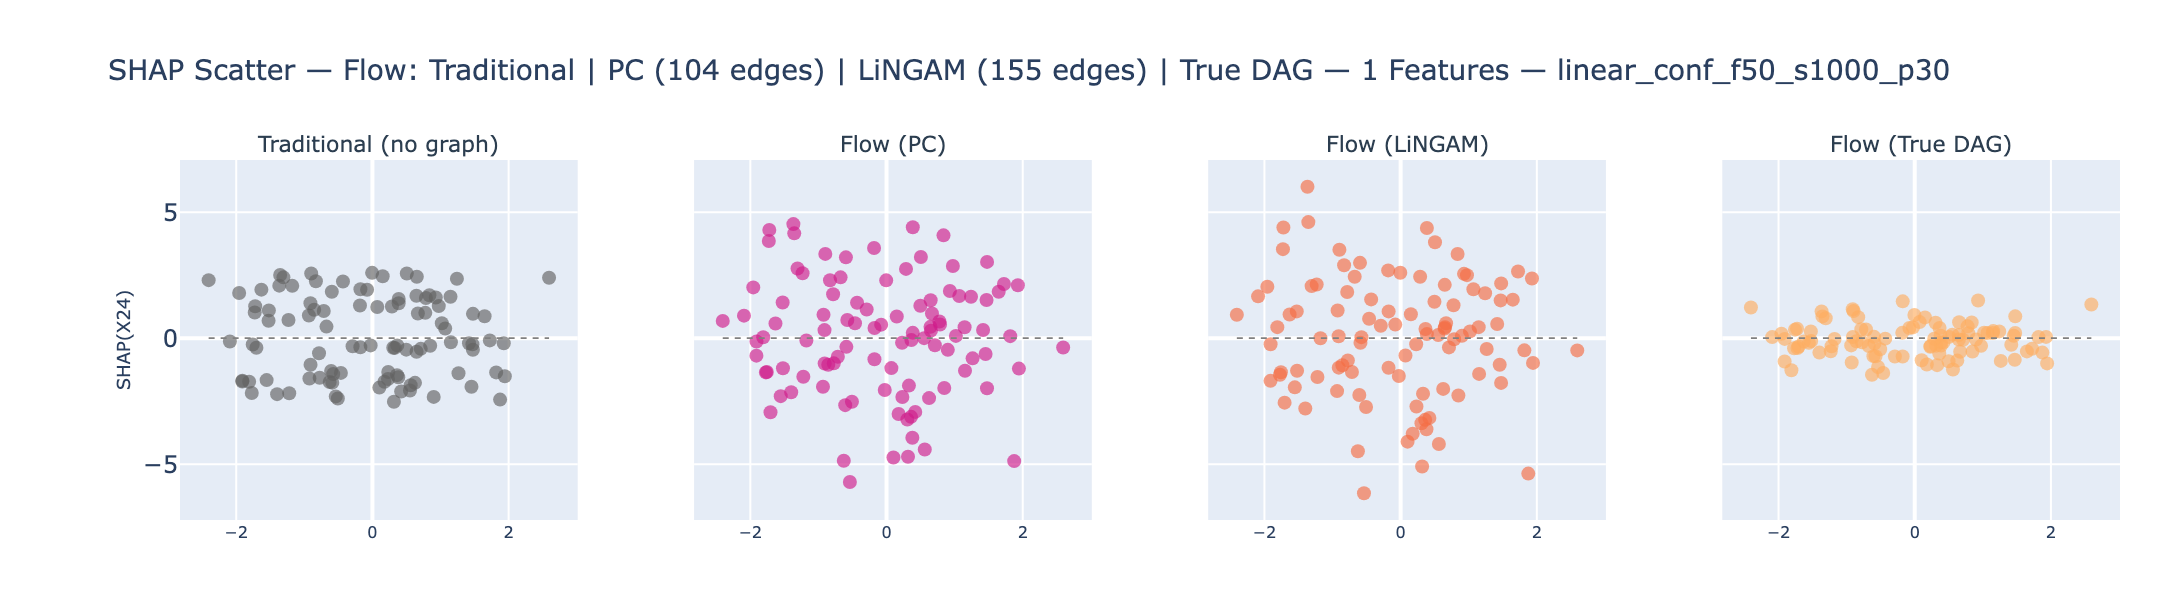
\includegraphics[width=\linewidth]{figures/shap_scatter_flow_X24_linear_conf_f50_s1000_p30.png}
  \caption{\textbf{Shapley Flow SHAP scatter (feature value vs.\ SHAP value) for X24 under Traditional (no graph), Flow+PC, Flow+LiNGAM and Flow+True DAG, synthetic dataset.} The Traditional column shows a stable attribution pattern; both discovered-graph columns diverge substantially from the True-DAG oracle, with inflated and partially sign-flipped values. The magnitude of this divergence, 32.5\% of $\hat{\sigma}$, is precisely the $\Delta M_{\text{base}}$ signal identified in Section~\ref{sec:baseline}, making this scatter a direct visualisation of why large feature-level baseline divergence should trigger structural validation of the discovered graph.}
  \label{fig:shap_X24}
\end{figure}

X47 shows the complementary pattern driven by edge reversal. In the True DAG it has 3 incoming and 1 outgoing edge. LiNGAM reverses its incoming edges and isolates it as an apparent root source, which causes Flow to inflate its attribution well above the oracle (feature-level $\Delta M_{\text{oracle}} = 41.2\%$ of $\hat{\sigma}$). PC, by contrast, recovers X47's incoming edges essentially correctly, and its feature-level $\Delta M_{\text{oracle}}$ is far lower (8.6\%). This split is visible in the Flow SHAP scatter: the X47 magnitudes under Flow+PC track Flow+True closely, while Flow+LiNGAM is widely inflated.

\begin{figure}[H]
  \centering
  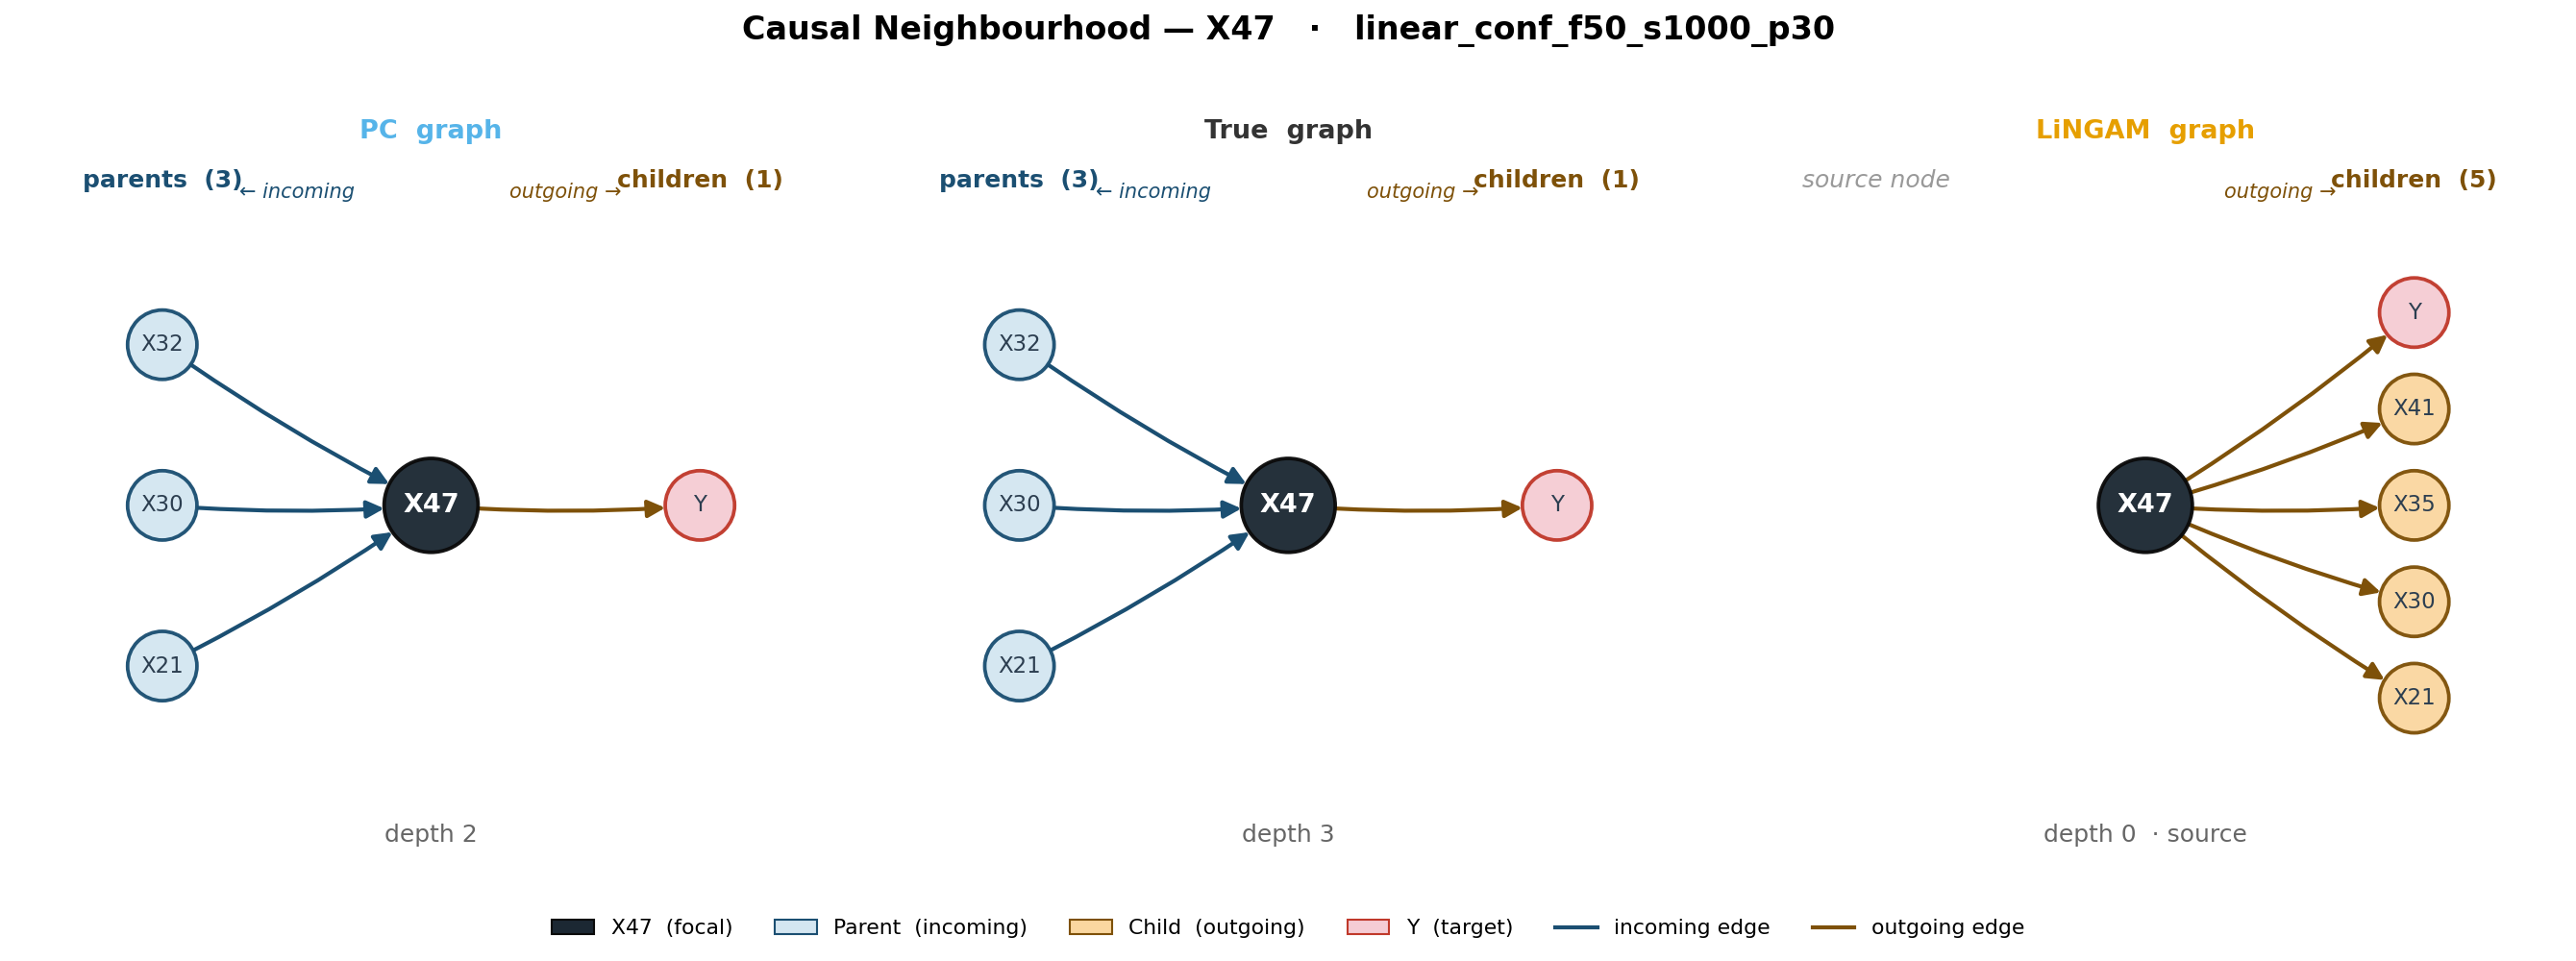
\includegraphics[width=\linewidth]{figures/dag_neighborhood_X47_linear_conf_f50_s1000_p30.png}
  \caption{\textbf{Causal neighbourhood of X47 across the PC (left), True DAG (centre), and LiNGAM (right) graphs, synthetic dataset.} PC recovers X47's incoming edges accurately (depth 2, 3 in-edges), whereas LiNGAM reverses them, leaving X47 as a 0-in / 5-out apparent source.}
  \label{fig:dag_X47}
\end{figure}

\begin{figure}[H]
  \centering
  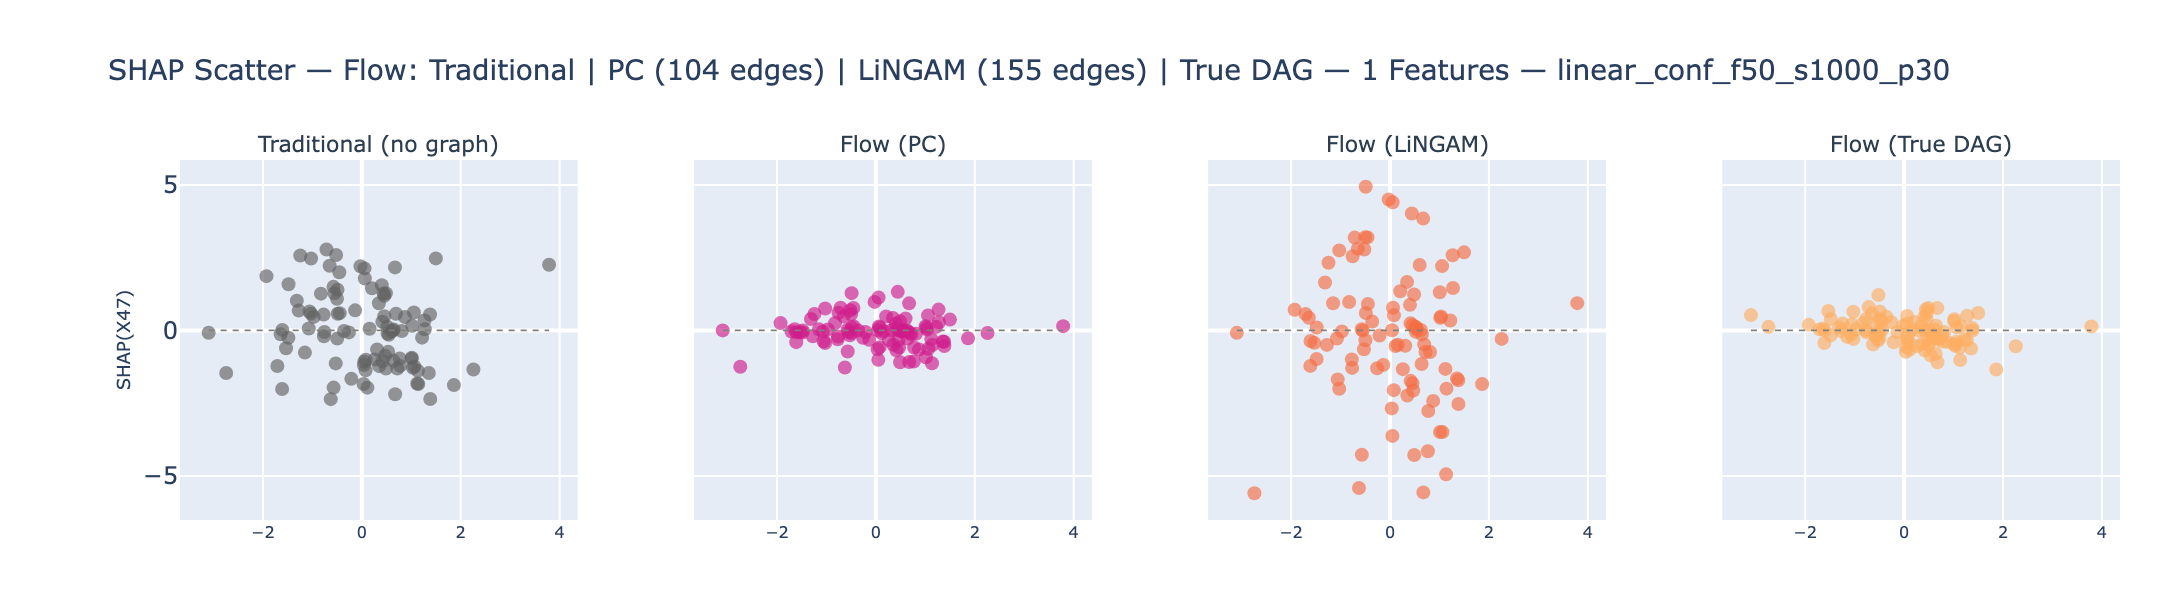
\includegraphics[width=\linewidth]{figures/shap_scatter_flow_X47_linear_conf_f50_s1000_p30.png}
  \caption{\textbf{Shapley Flow SHAP scatter for X47.} Flow+PC and Flow+True columns show closely matching magnitudes, while Flow+LiNGAM is visibly inflated---the scatter-level signature of reversal-induced root-source overloading.}
  \label{fig:shap_X47}
\end{figure}

The same mechanism appears on Sachs through protein pka (Figure~\ref{fig:dag_pka}). pka is a dominant predictor and near-root source (1 incoming, 6 outgoing edges in the consensus DAG). LiNGAM keeps it almost correct, a pure root with 7 outgoing edges, giving an Asymmetric $\Delta M_{\text{oracle}}$ of just 6.4\% of $\hat{\sigma}$, whereas PC reverses several outgoing edges into a 3-in/3-out node, and that mis-orientation cascades downstream to raise pka's Asymmetric $\Delta M_{\text{oracle}}$ to 25.0\%. The asymmetry carries to Flow, where Flow+LiNGAM tracks the oracle but Flow+PC underestimates pka's explainability.

The diagnostic signals for pka are present before the oracle is consulted. At the feature level, $\Delta M_{\text{base}}$ reaches 17.3\% of $\hat{\sigma}$ for at least one Shapley method, placing pka among the highest-deviating proteins relative to the Traditional Shapley baseline (visible in Figure~\ref{fig:heatmap_trad}). This alone warrants closer inspection of pka's discovered connections: a node whose attributions shift that far from the graph-free baseline is one where the injected graph structure is doing significant work, and that work may be misdirected if the discovered edges are unreliable. Compounding this, the feature-level $\Delta M_{\text{disc}}$ for pka (Figure~\ref{fig:gss}) reveals a large discrepancy between what PC and LiNGAM assign to the protein, the two discovery algorithms disagree substantially on its neighbourhood, and that disagreement propagates directly into attribution instability. Together, a high $\Delta M_{\text{base}}$ and a high $\Delta M_{\text{disc}}$ on the same node serve as a two-signal alarm: the discovered causal connections of that feature are both influential and contested. A practitioner encountering this pattern should either research further the causal relations obtained for the specific edges flagged (in pka's case, whether it truly acts as a near-root source or receives inputs from upstream regulators), or consider constraining the discovery output, for instance by enforcing known biological orientation constraints or by increasing the algorithm's confidence tolerance before trusting the resulting Shapley attributions.

\begin{figure}[H]
  \centering
  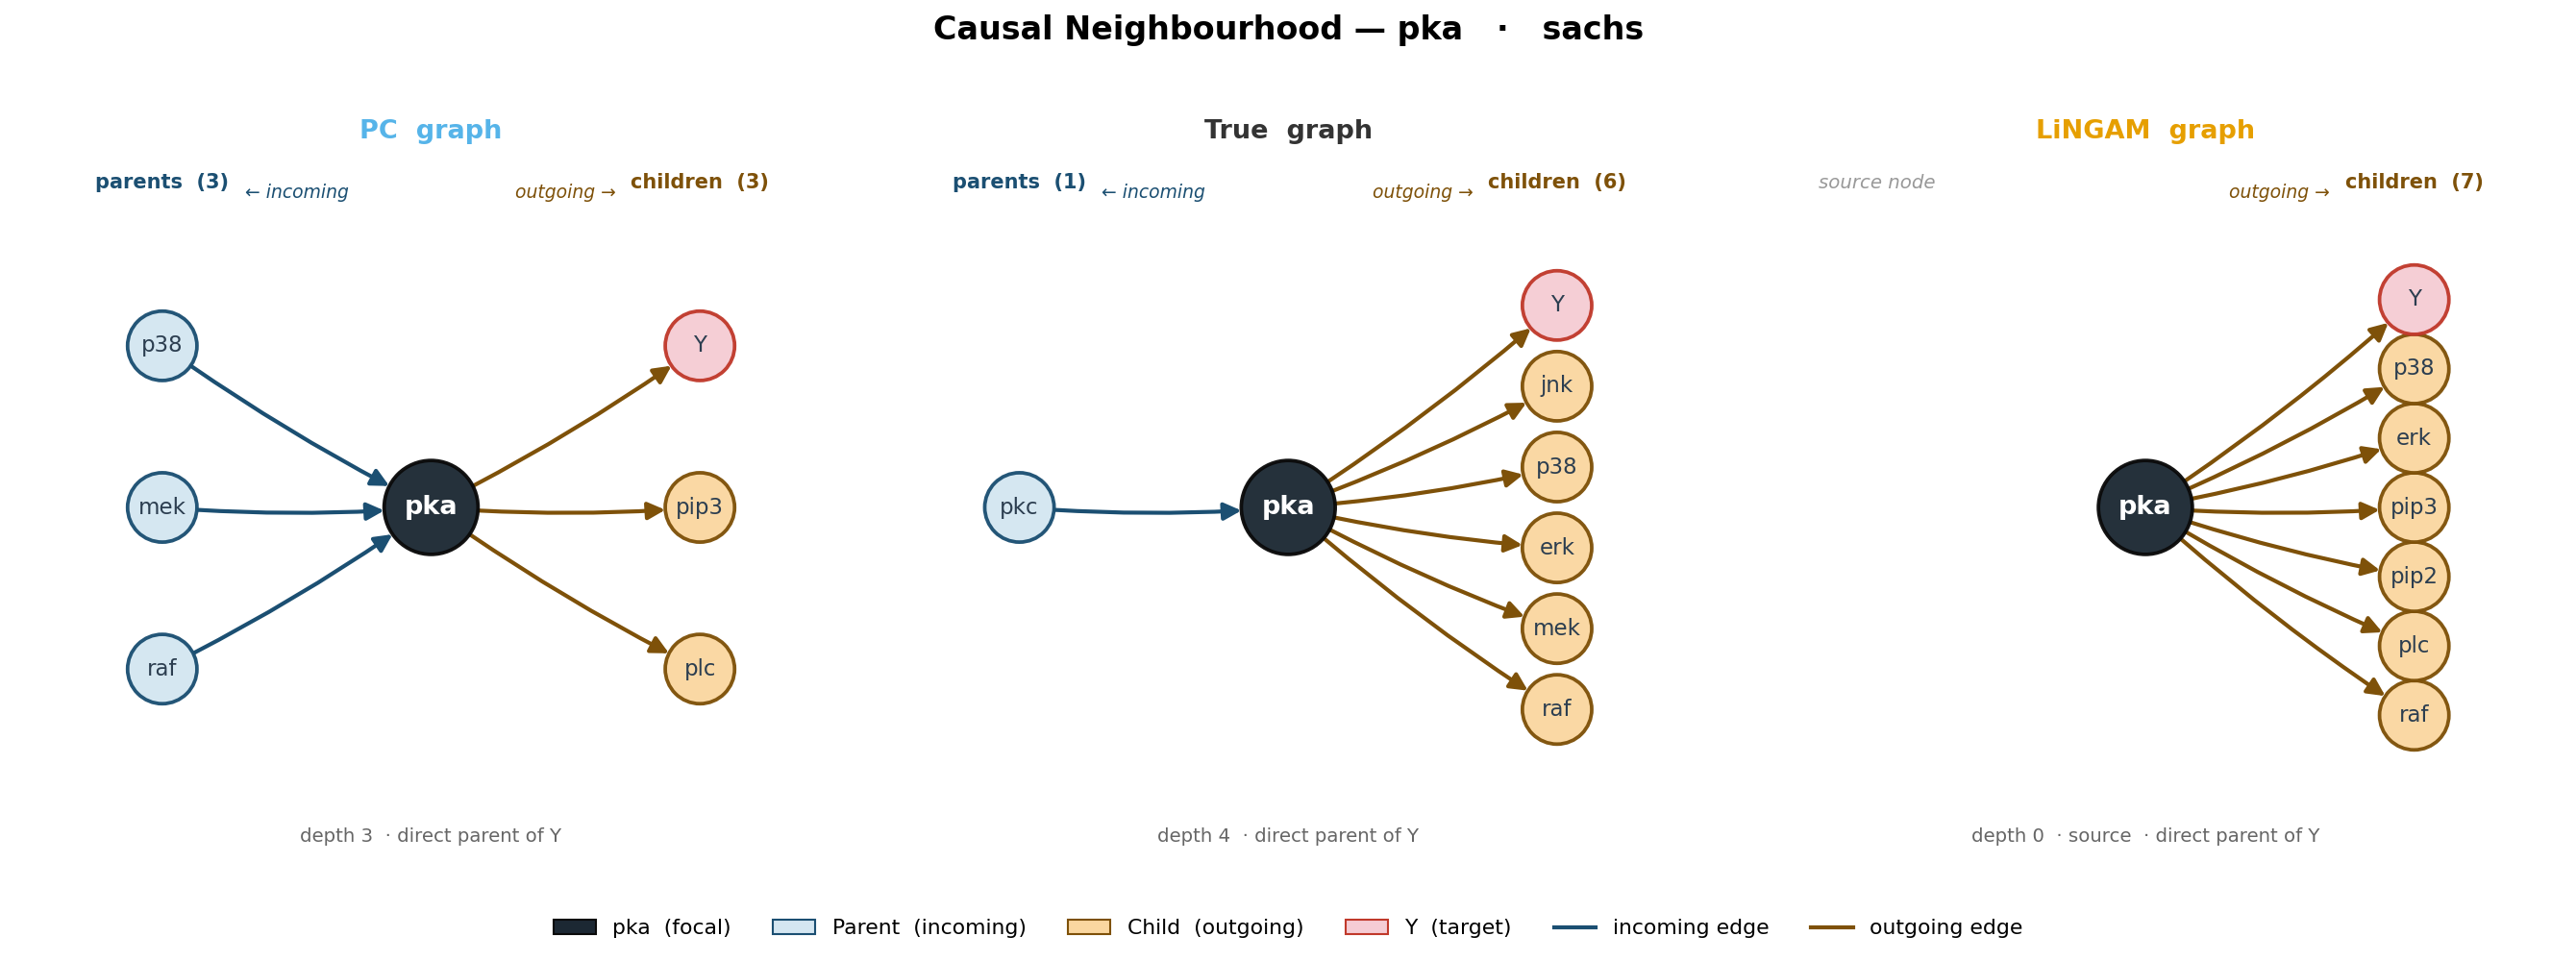
\includegraphics[width=\linewidth]{figures/dag_neighborhood_pka_sachs.png}
  \caption{\textbf{Causal neighbourhood of pka across the PC (left), True DAG (centre), and LiNGAM (right) graphs, Sachs dataset.} pka is a near-root source with 1 incoming and 6 outgoing edges in the consensus DAG. PC gives pka 3 incoming and 3 outgoing edges (reversing several true outgoing links), while LiNGAM keeps it a pure root with 7 outgoing edges and none incoming, much closer to the consensus structure. The PC reversal that adds spurious incoming edges drives its $\Delta M_{\text{oracle}}$ from 6.4\% of $\hat{\sigma}$ (LiNGAM) up to 25.0\% (PC).}
  \label{fig:dag_pka}
\end{figure}

\subsubsection{Directed Edge Inversion and Causal Credit Transfer}

This mechanism illustrates how a single edge orientation error by one discovery algorithm produces a divergent attribution pattern relative to the other algorithm and relative to the oracle. In the True DAG the edge runs $X_{21} \to X_{47}$: X21 is a causal ancestor of X47, which in turn is a dominant direct parent of $Y$. LiNGAM recovers this orientation correctly. PC, by contrast, reverses it to $X_{47} \to X_{21}$, transforming X47 from X21's child into its apparent parent.

The consequences for attributions split sharply across the two graphs. Under LiNGAM, both Causal Shapley and Shapley Flow correctly treat X21 as an upstream node: X21 receives some indirect credit for its causal influence on X47 and through it on $Y$, a sensible allocation given the true generative structure. Under PC the reversed edge places X47 upstream of X21; in Causal Shapley this injects X47 into X21's interventional parent set, altering X21's post-interventional distribution and contaminating both attributions, while in Flow the outgoing edge $X_{47} \to X_{21}$ routes a share of X47's credit toward X21, reducing X47's net attribution and inflating X21's. The result is that the PC and LiNGAM variants disagree substantially: X47 is under-attributed under PC relative to the oracle, while LiNGAM and True DAG agree closely.

The diagnostic signals are present before the oracle is consulted. Feature-level $\Delta M_{\text{base}}$ flags X47 as having elevated divergence from the Traditional Shapley baseline, and feature-level $\Delta M_{\text{disc}}$ highlights it as one of the nodes with the largest magnitude gap between the PC and LiNGAM variants (reaching 29.8\% of $\hat{\sigma}$ for CSV). Together these two signals identify X47 as a feature where the discovered causal structure is doing substantial and contested work. The practical lesson this case illustrates is that the appropriate response to such a signal is not to prune the discovered edge between X21 and X47 as the first option, the edge is genuine, but to invest in resolving its correct orientation before running the structure-aware Shapley computation. Removing a real causal link would impoverish the graph and suppress legitimate indirect-effect attribution, whereas correcting the orientation (as LiNGAM achieves here) restores oracle-consistent explanations without discarding structural information.

\begin{figure}[H]
  \centering
  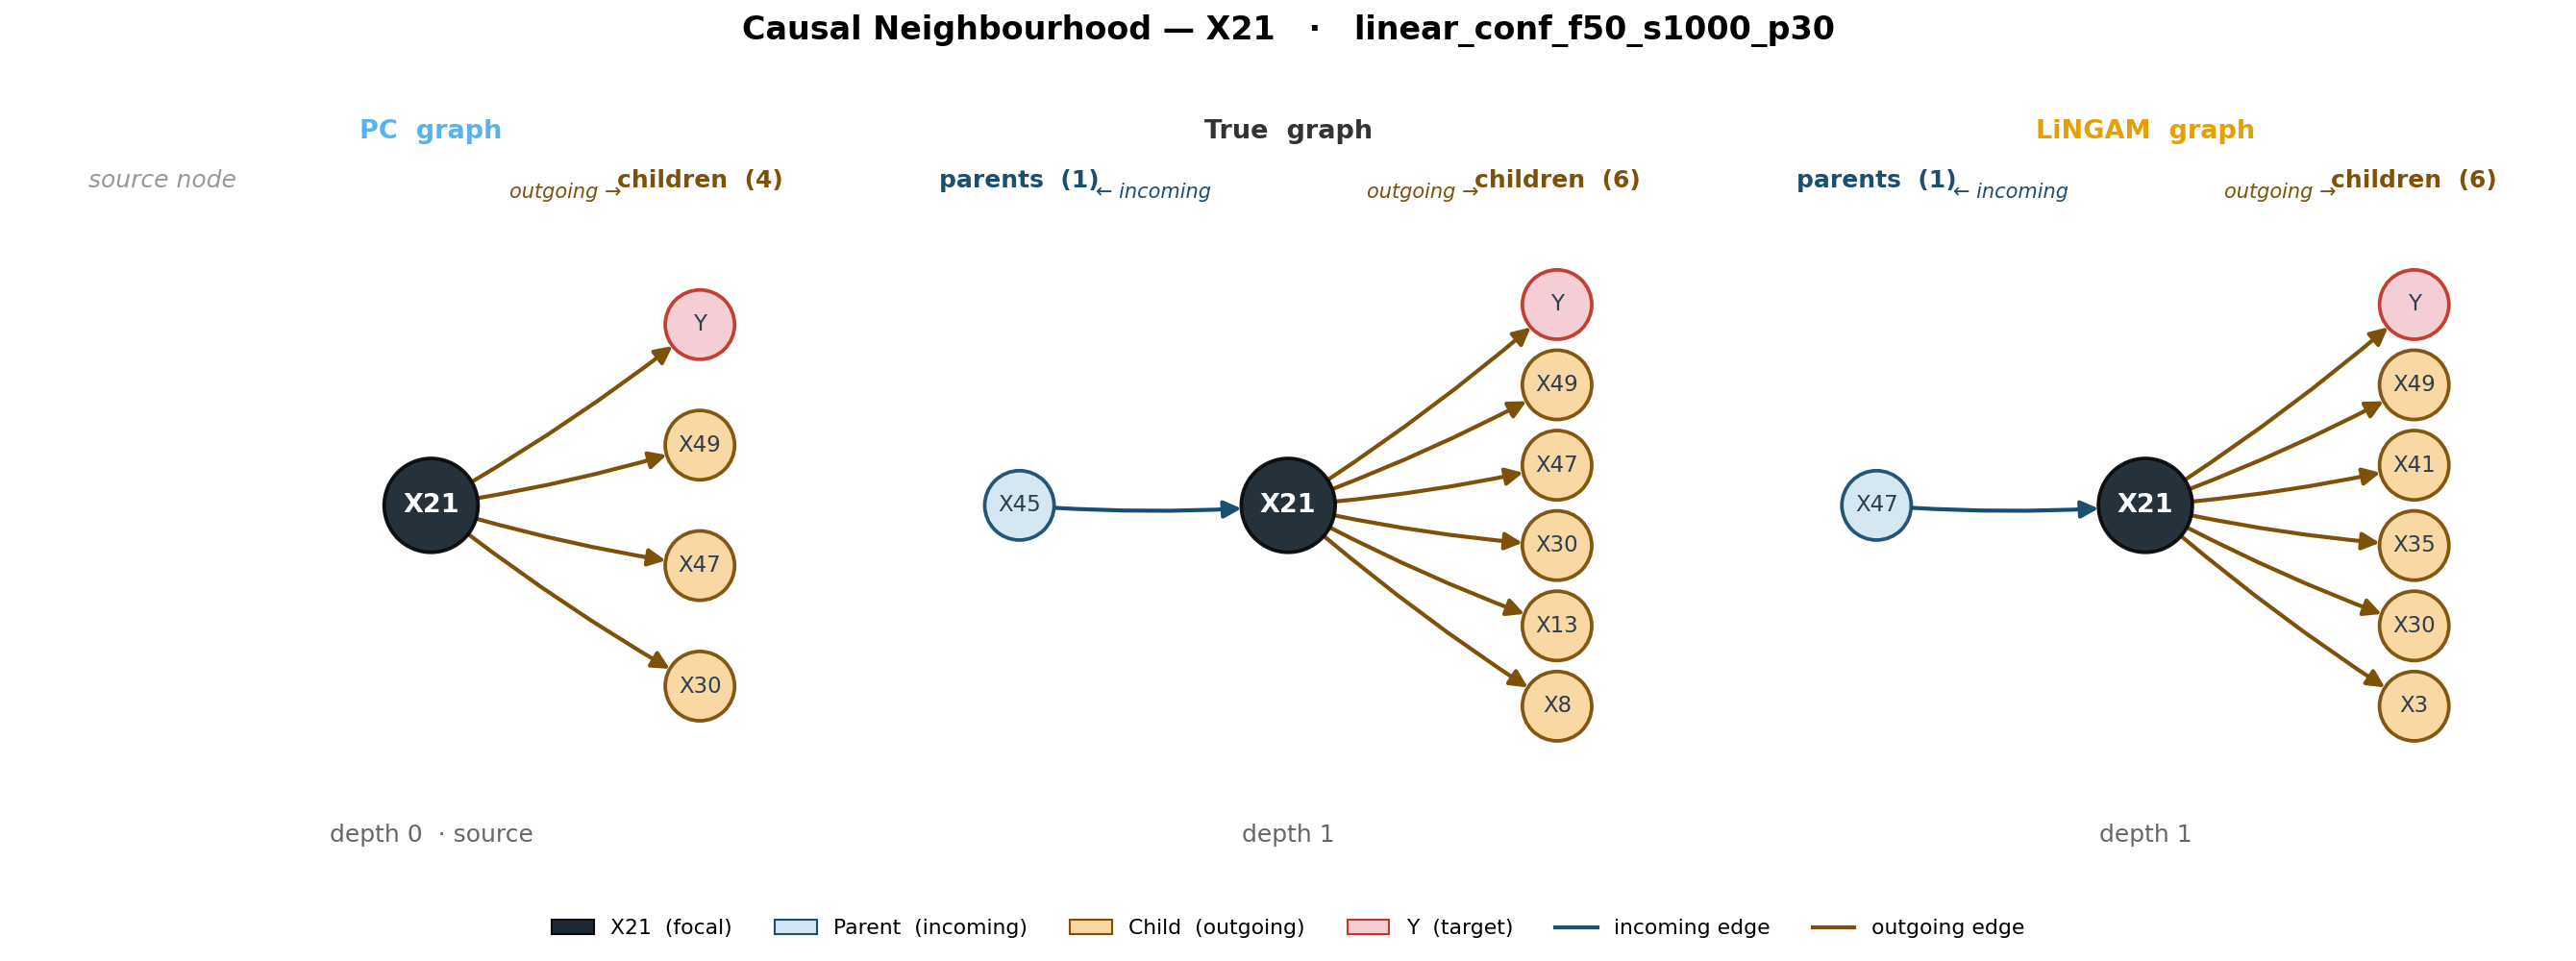
\includegraphics[width=0.85\linewidth]{figures/dag_neighborhood_X21_linear_conf_f50_s1000_p30.png}
  \caption{\textbf{Causal neighbourhood of X21 across the PC (left), True DAG (centre), and LiNGAM (right) graphs, synthetic dataset.} In the True DAG and under LiNGAM, the edge runs $X_{21} \to X_{47}$. PC reverses it to $X_{47} \to X_{21}$, placing X47 upstream of X21 and misdirecting attribution credit in both Causal Shapley and Flow.}
  \label{fig:dag_X21}
\end{figure}

\begin{figure}[H]
  \centering
  \begin{subfigure}[t]{0.48\linewidth}
    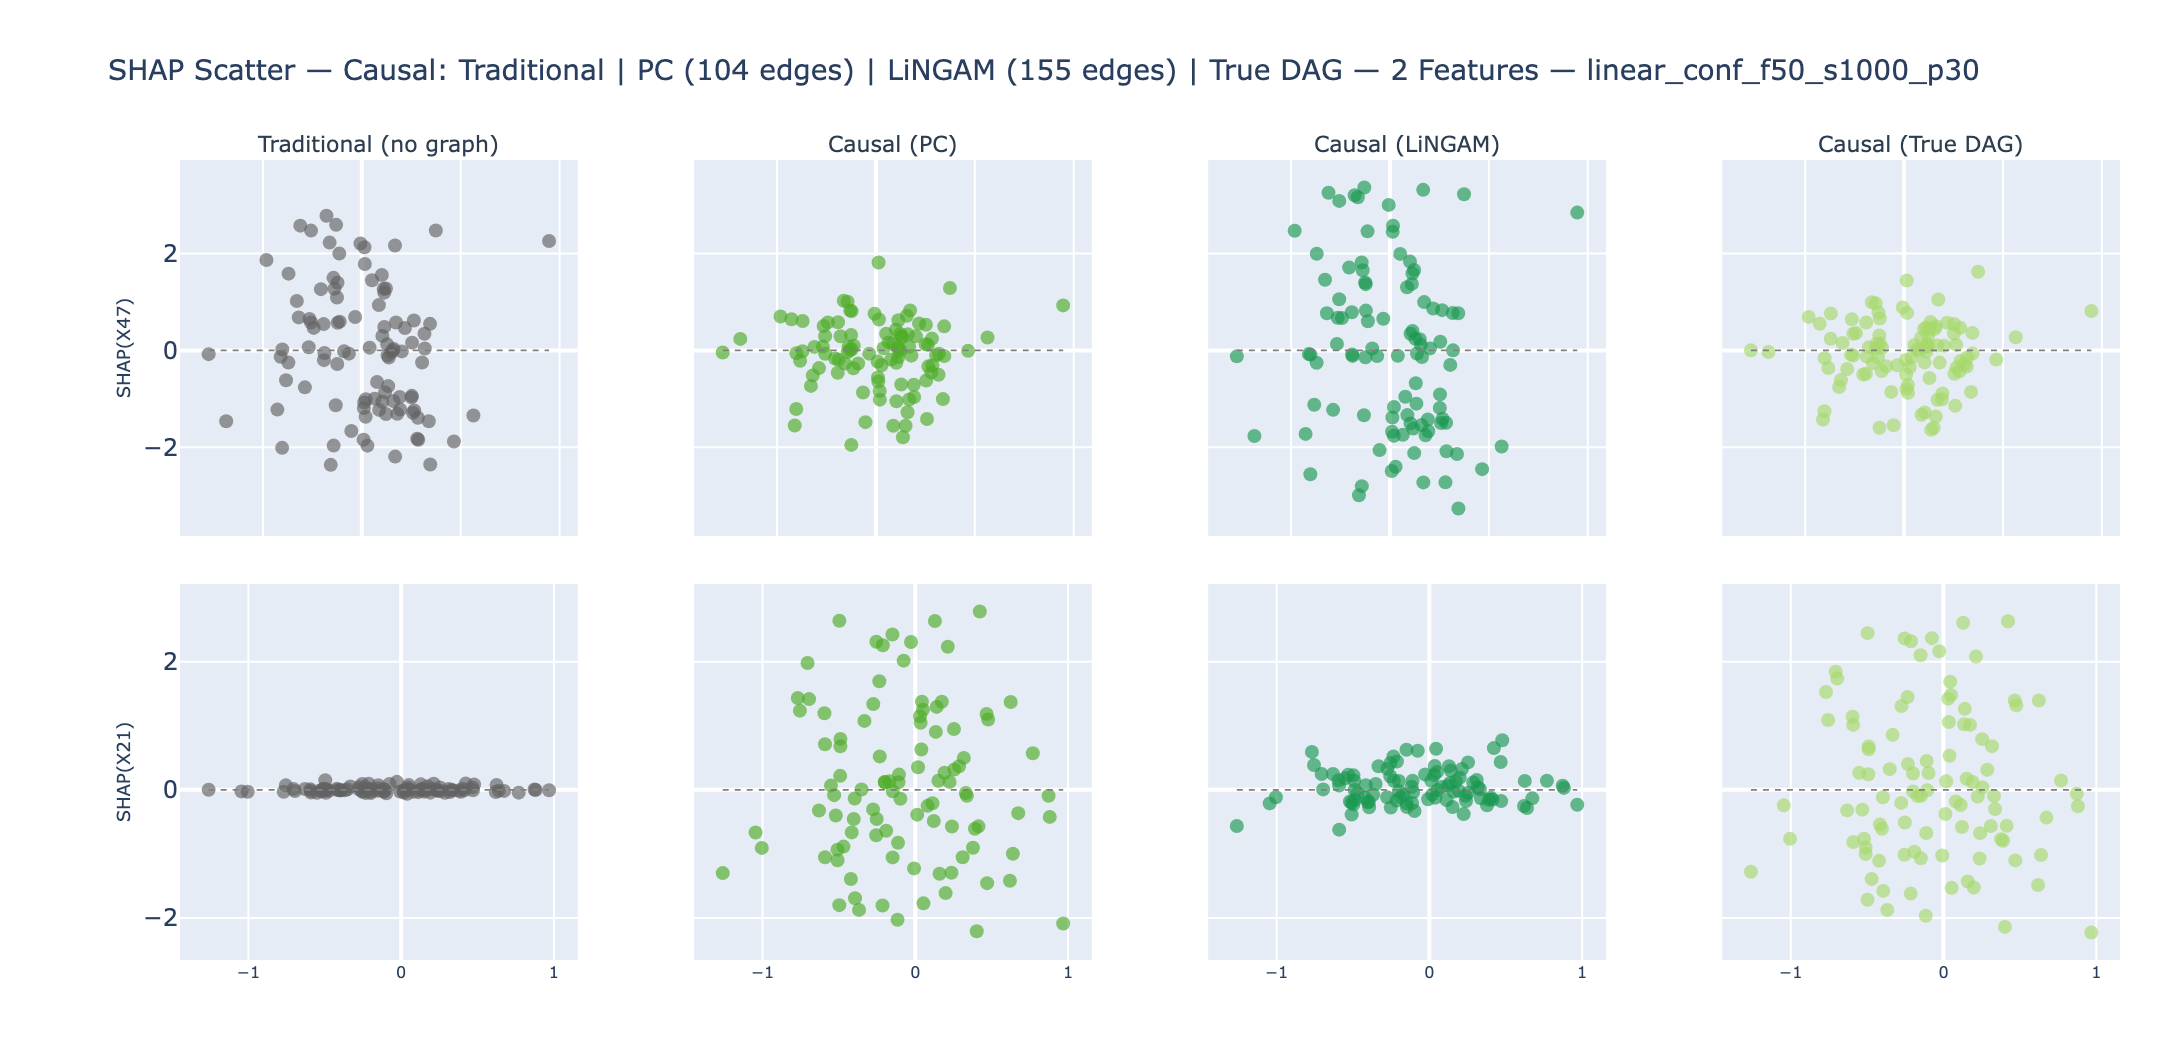
\includegraphics[width=\linewidth]{figures/shap_scatter_causal_X47_X21_linear_conf_f50_s1000_p30.png}
    \caption{Causal Shapley: under LiNGAM (correct orientation) both X21 and X47 attributions track the oracle. Under PC (reversed orientation), X47 is suppressed and X21 acquires inflated credit.}
    \label{fig:shap_X47_X21_causal}
  \end{subfigure}
  \hfill
  \begin{subfigure}[t]{0.48\linewidth}
    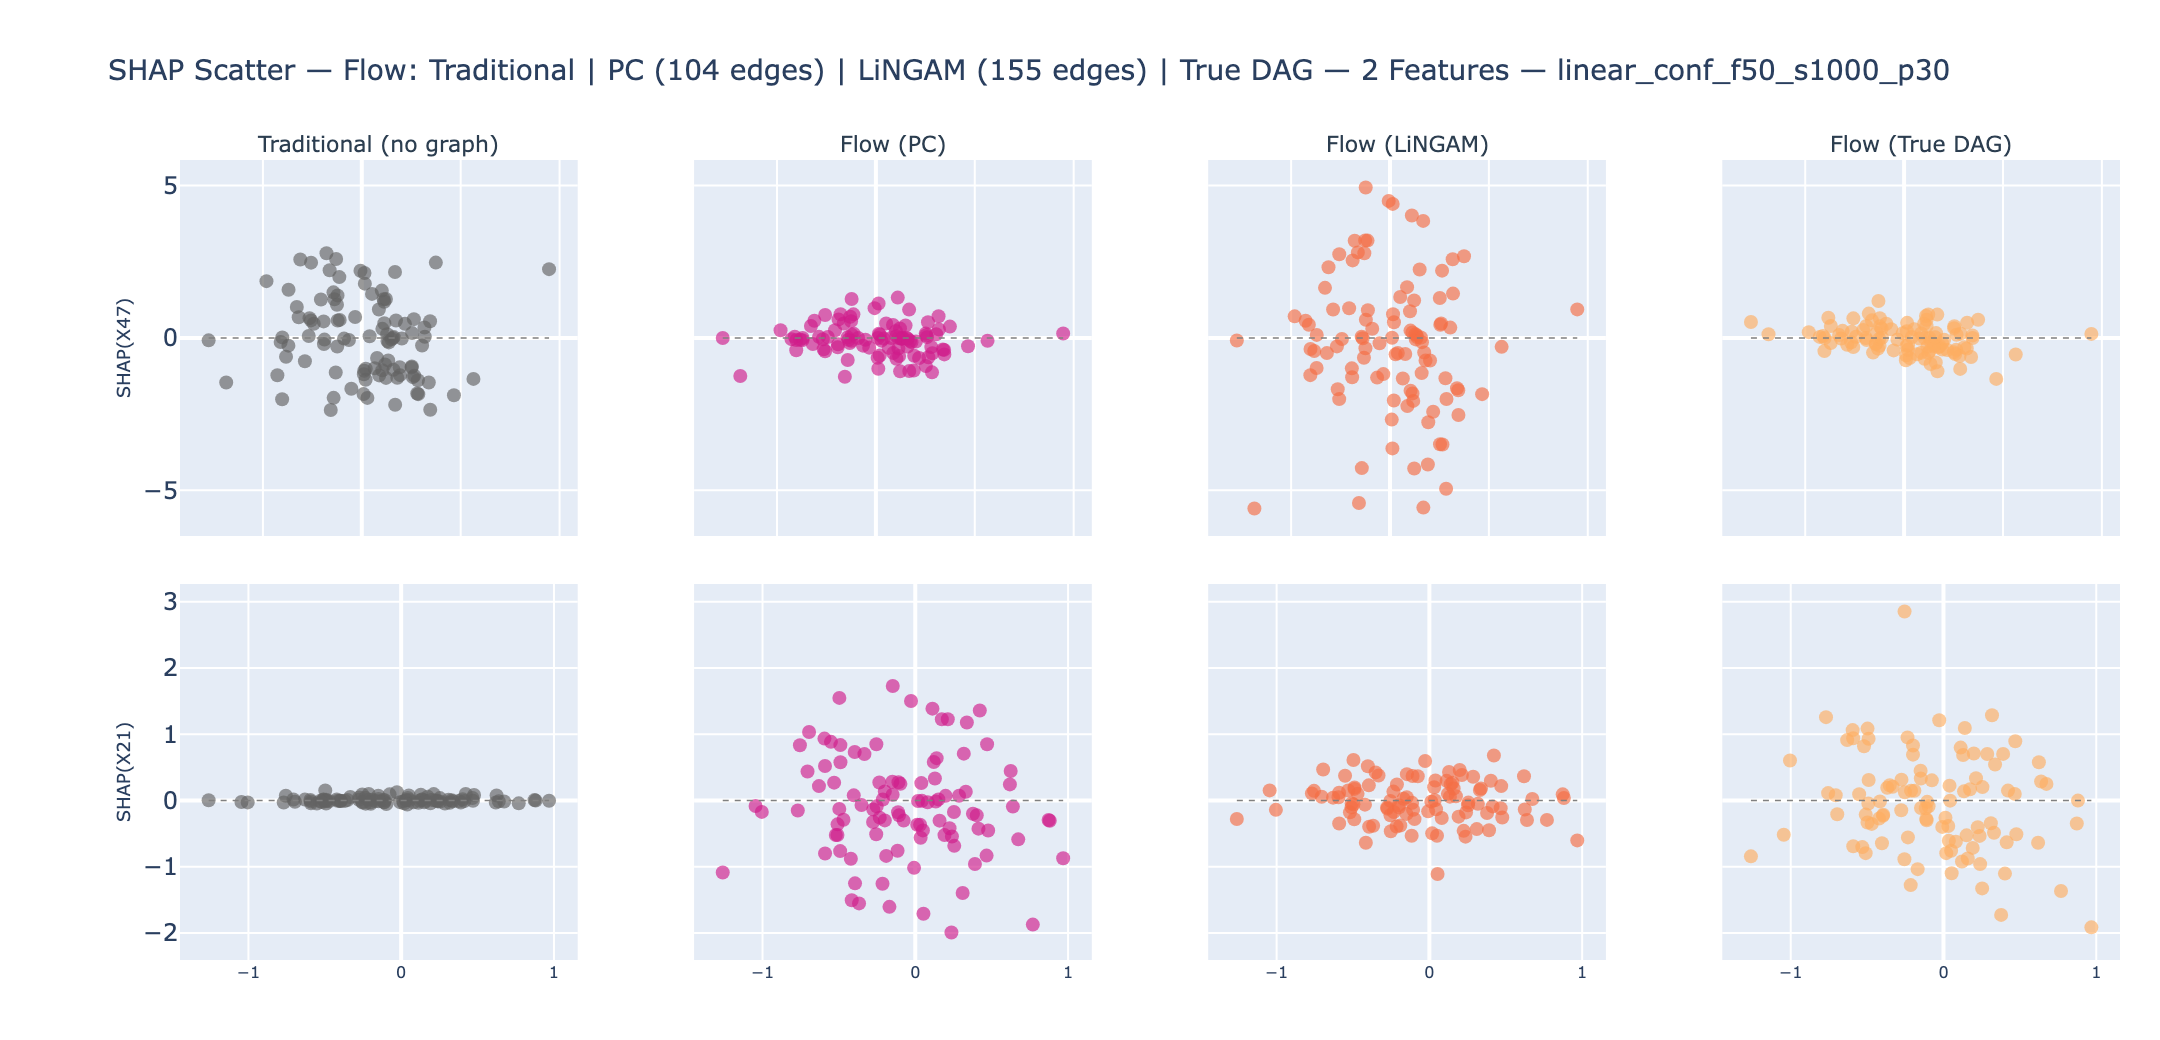
\includegraphics[width=\linewidth]{figures/shap_scatter_flow_X47_X21_linear_conf_f50_s1000_p30.png}
    \caption{Shapley Flow: the same orientation-driven credit transfer appears; Flow+LiNGAM and Flow+True agree closely, while Flow+PC diverges on both features.}
    \label{fig:shap_X47_X21_flow}
  \end{subfigure}
  \caption{\textbf{SHAP scatter for X21 and X47 across graph configurations.}}
  \label{fig:shap_X47_X21}
\end{figure}

\subsubsection{Confounded Subordination and Boundary Isolation}

Synthetic feature X6 is a true intermediate channel with 3 parents and 4 children. Under LiNGAM its parent set is inflated by roughly eight false incoming links (in-degree 8 in the LiNGAM graph against 3 in the True DAG), and under CSV these false parents generate an overly constrained post-interventional distribution for X6, yielding a feature-level $\Delta M_{\text{oracle}} = 28.1\%$ of $\hat{\sigma}$, among the highest in the synthetic confounded track. X6 is a clean illustration of LiNGAM's poor precision and recall translating directly into attribution error: because the discovery algorithm attributes far more incoming connections to the node than truly exist, the interventional conditioning set is contaminated, and the discovery-quality failure becomes a Causal Shapley failure. This makes the precision and recall of the discovery step a direct and visible factor in CSV's reliability.

\begin{figure}[H]
  \centering
  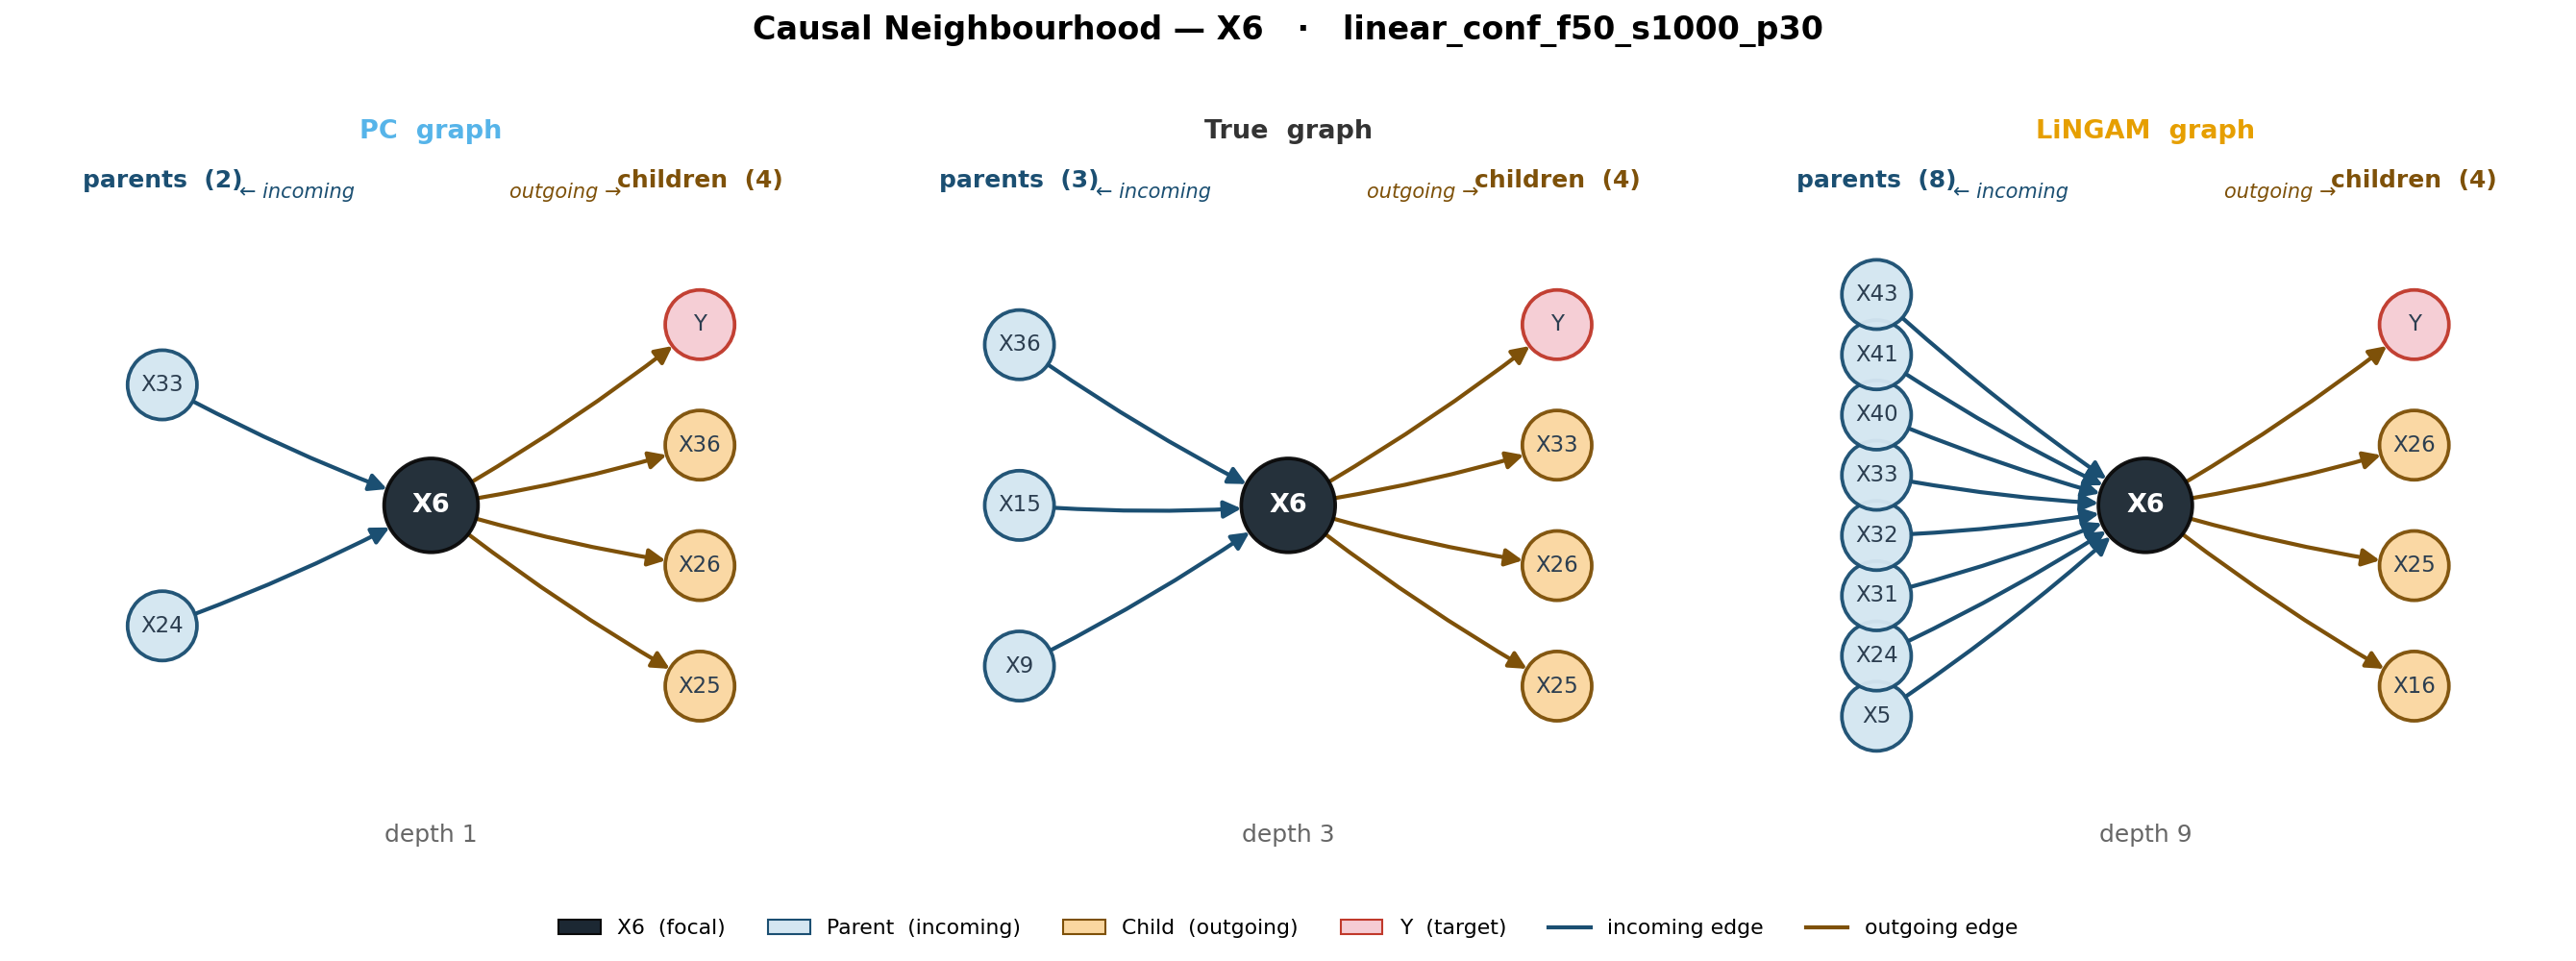
\includegraphics[width=0.85\linewidth]{figures/dag_neighborhood_X6_linear_conf_f50_s1000_p30.png}
  \caption{\textbf{Causal neighbourhood of X6 across the PC (left), True DAG (centre), and LiNGAM (right) graphs, synthetic dataset.} X6 is a genuine intermediate node with 3 incoming and 4 outgoing edges in the True DAG. LiNGAM inflates its in-degree to 8, the over-connection that contaminates its interventional parent set under Causal Shapley.}
  \label{fig:dag_X6}
\end{figure}

\begin{figure}[H]
  \centering
  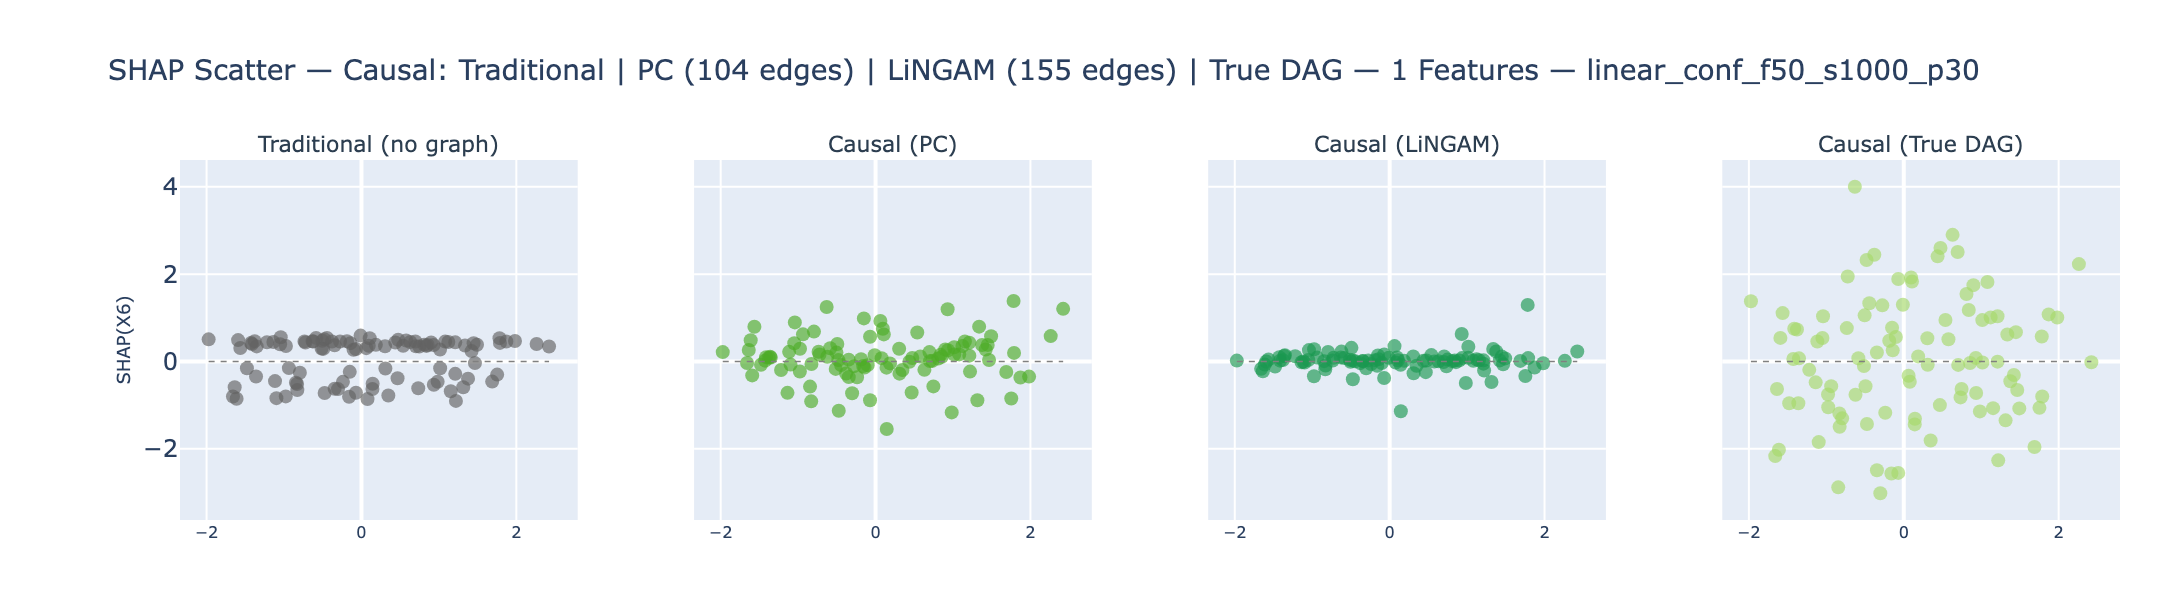
\includegraphics[width=\linewidth]{figures/shap_scatter_causal_X6_linear_conf_f50_s1000_p30.png}
  \caption{\textbf{Causal Shapley SHAP scatter for X6 across Traditional (no graph), Causal+PC, Causal+LiNGAM and Causal+True DAG, synthetic dataset.} The LiNGAM column diverges substantially from both the Traditional baseline and the True DAG oracle, while PC stays close to the oracle---a direct consequence of LiNGAM inflating X6's in-degree from 3 to 8 and contaminating its interventional conditioning set.}
  \label{fig:shap_X6}
\end{figure}

The instance-level effect of this in-degree inflation confirms that under Causal Shapley, the LiNGAM column diverges sharply from both the Traditional baseline and the True DAG oracle: the spurious parent set forces do-distributions conditioned on eight nodes rather than three, producing attributions that neither reflect the graph-free model behaviour nor the causally correct one. Causal Shapley under PC, by contrast, stays much closer to the True DAG column, consistent with PC's more conservative graph on this feature. This makes X6 a clean example of how LiNGAM's poor edge precision---a discovery metric, not an attribution metric---directly degrades the downstream explanation quality under interventional methods.

On the Sachs dataset, protein erk is a downstream node that in the consensus DAG receives inputs from pka and mek. PC discovers a markedly different configuration, removing erk's parent links and isolating it as an apparent root node with several outgoing edges. Under Shapley Flow this isolation assigns erk a disproportionately large attribution, because with no incoming edges and many outgoing ones it accumulates outgoing-edge credit that the true structure would have distributed to its parents (feature-level $\Delta M_{\text{oracle}} = 49.2\%$ of $\hat{\sigma}$ for Flow+PC, the largest in the real-data experiment).

\begin{figure}[H]
  \centering
  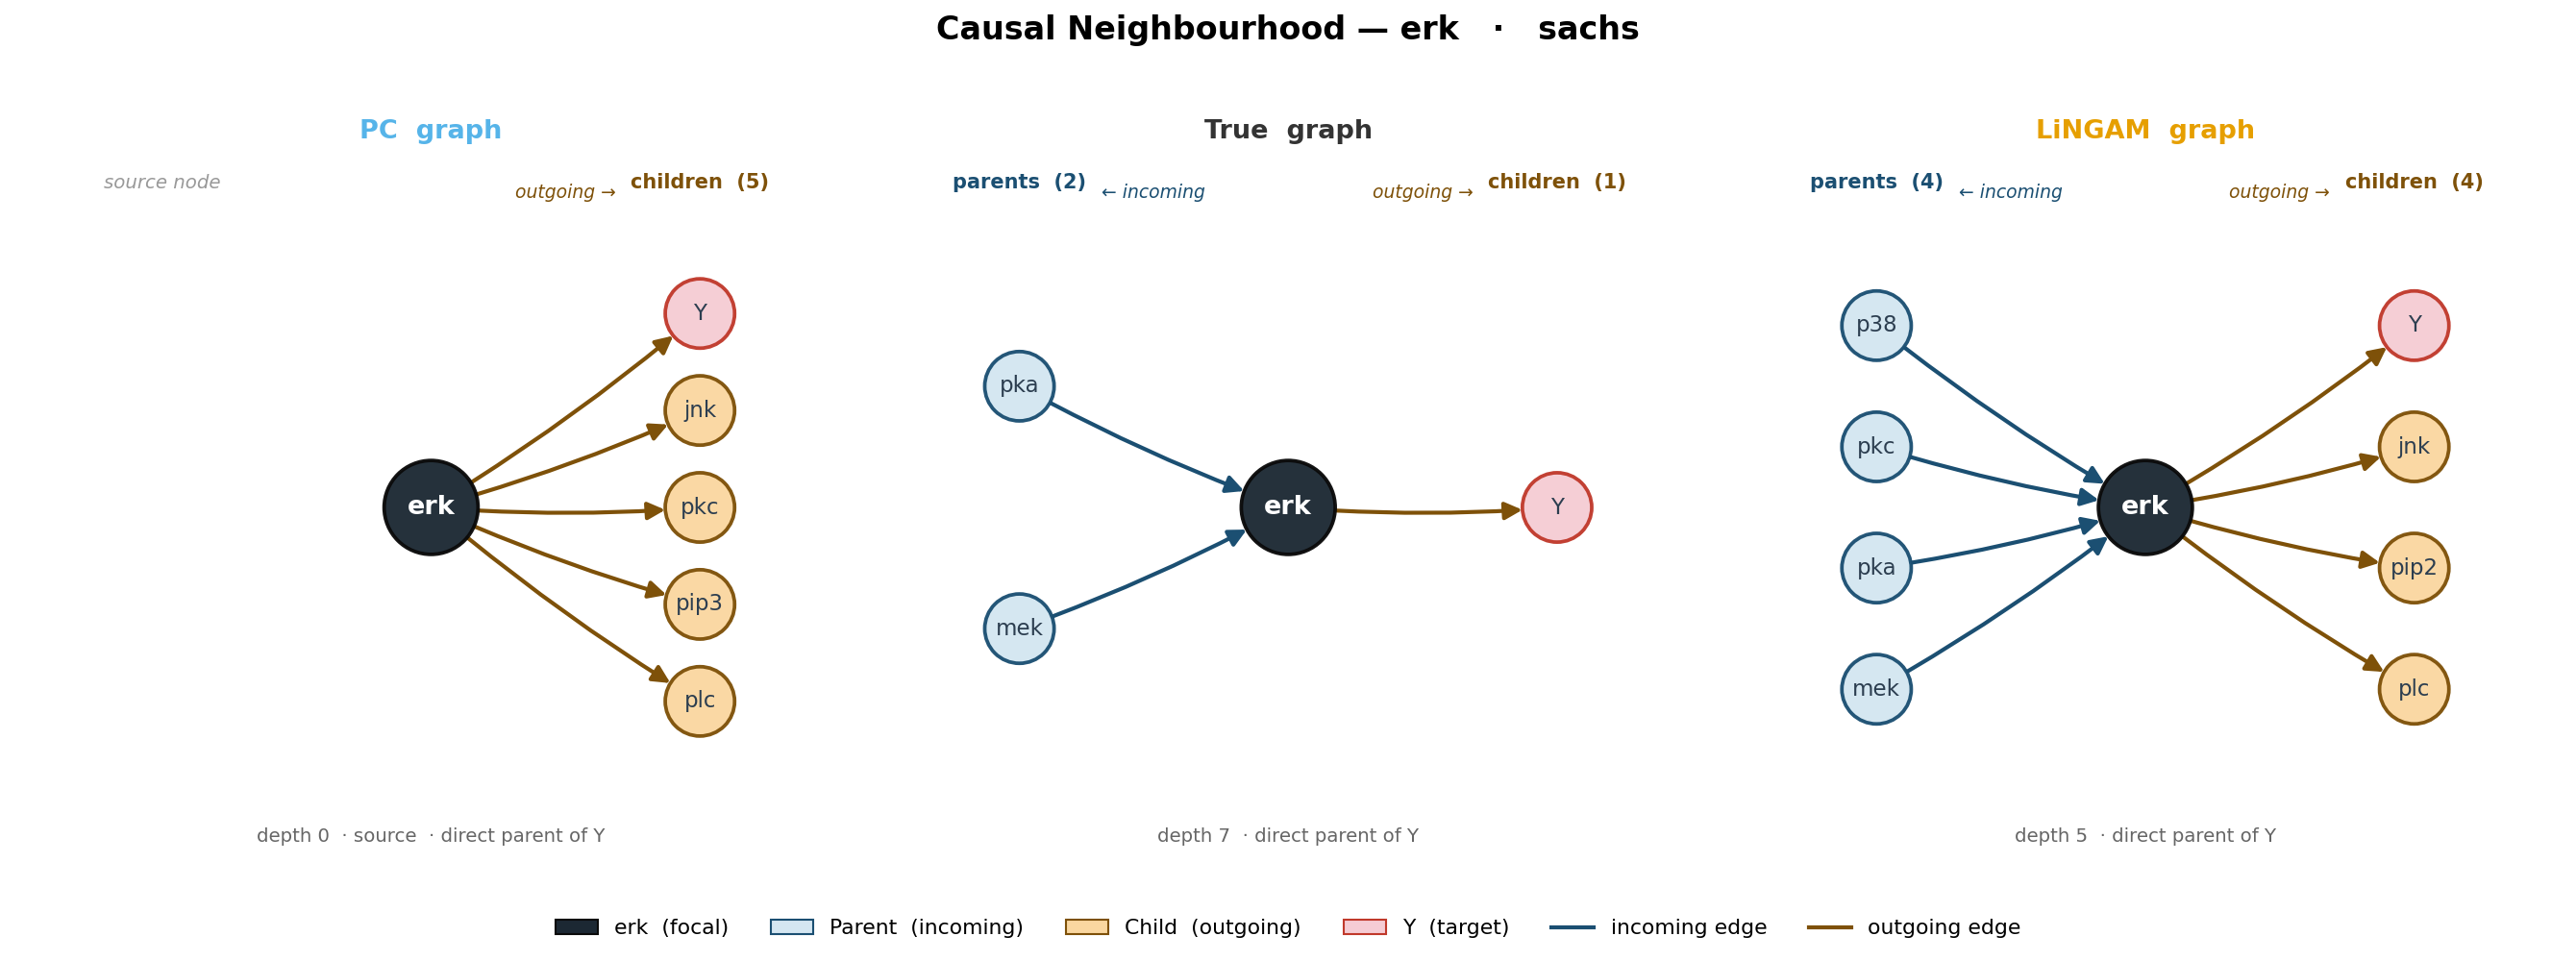
\includegraphics[width=\linewidth]{figures/dag_neighborhood_erk_sachs.png}
  \caption{\textbf{Causal neighbourhood of erk across the PC (left), True DAG (centre), and LiNGAM (right) graphs, Sachs dataset.} In the consensus DAG erk is a downstream node receiving inputs from pka and mek. PC removes its true incoming edges and leaves it with outgoing edges only, recasting a downstream node as a boundary source, the mis-orientation that drives Flow+PC's feature-level $\Delta M_{\text{oracle}}$ of 49.2\% of $\hat{\sigma}$.}
  \label{fig:dag_erk}
\end{figure}

\begin{figure}[H]
  \centering
  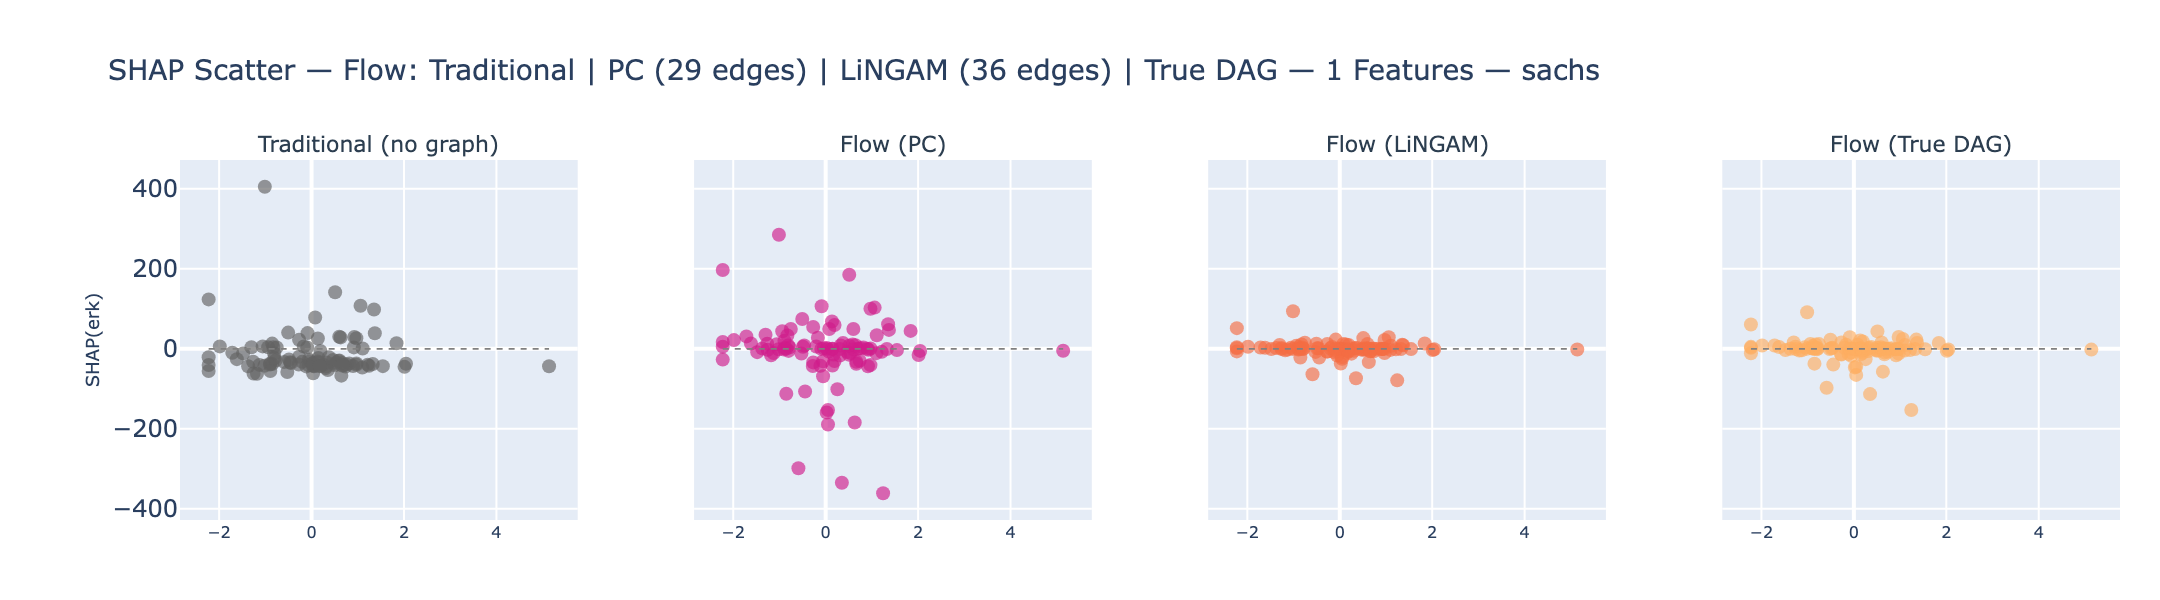
\includegraphics[width=\linewidth]{figures/shap_scatter_flow_erk_sachs.png}
  \caption{\textbf{Shapley Flow SHAP scatter for erk, Sachs dataset.} All three graph-aware variants diverge from each other and from the Traditional baseline. Flow+PC inflates erk's attributions by treating it as a source node; Flow+LiNGAM produces a distinct distortion; only Flow+True DAG tracks the correct downstream credit distribution. The simultaneous divergence on $\Delta M_{\text{base}}$, $\Delta M_{\text{oracle}}$, and $\Delta M_{\text{disc}}$ marks erk as a node where structure-aware methods should not be deployed without prior graph validation.}
  \label{fig:shap_erk}
\end{figure}

The instance-level consequences of these conflicting graph configurations are visible in the Flow Shapley scatter for erk. All three variants---Flow+PC, Flow+LiNGAM, and Flow+True DAG---produce materially different attribution patterns. Flow+PC assigns erk a systematically inflated attribution cluster, consistent with PC treating it as an isolated source node that collects all outgoing-edge credit. Flow+LiNGAM produces a different distortion: LiNGAM recovers some incoming edges for erk but the overall topology still diverges from the consensus DAG, resulting in attributions that are neither close to the PC column nor to the True DAG oracle. The True DAG column behaves differently from both, distributing credit across erk's correct parent links and pulling the overall attribution level down. Across all three metrics, $\Delta M_{\text{base}}$, $\Delta M_{\text{oracle}}$, and $\Delta M_{\text{disc}}$, erk is simultaneously far from the graph-free baseline, far from the oracle, and far from itself under a different causal discovery algorithm. This triple divergence is the clearest warning signal the framework can emit: it indicates that erk's edge configuration is not stable enough across discovery algorithms to justify any structure-aware Shapley method without first resolving the graph uncertainty through domain-expert validation or a more reliable discovery procedure.

%% ============================================================
\section{Conclusion}
\label{sec:conclusion}
%% ============================================================

\subsection{Summary of Findings}

This thesis built an experimental pipeline to measure what happens to feature attributions when an automatically discovered causal graph is plugged into a structure-aware Shapley method. The pipeline runs three Shapley methods (ASV, CSV, and Shapley Flow) under two discovered graphs (PC and LiNGAM) and the True DAG as an oracle, across a controlled 50-feature synthetic dataset and the real-world Sachs cell signaling dataset. The evaluation framework introduces six metrics organized by two dimensions: magnitude of change ($\Delta M$) and sign change ($D$), each measured at three levels: against the graph-free Traditional Shapley baseline, against the True DAG oracle, and as cross-discovery sensitivity between PC and LiNGAM.

The three Shapley methods occupy completely different sensitivity regimes. ASV is stable under graph errors, especially in sparse and high-dimensional datasets: on the 50-feature synthetic data, swapping the True DAG for an imprecise discovered graph moves ASV's attributions by less than $1.1\%$ of $\hat{\sigma}$ ($\Delta M_{\text{oracle}} < 1.1\%$, $D_{\text{oracle}} < 6.3\%$) and flips fewer than $7\%$ of attribution signs. This holds even on Sachs where LiNGAM's graph is barely decent (F1 = 0.326): ASV still keeps $\Delta M_{\text{oracle}} = 2.84\%$ of $\hat{\sigma}$, well under 4\% of the model-output standard deviation. This stability derives entirely from the algorithm's core logic: ASV's observational marginalization means that in a sparse high-dimensional graph, most topological orderings remain compatible across the true and discovered graphs, so the attribution values barely move. CSV and Flow's core logic moves beyond just affecting the ordering. CSV conditions on an interventional distribution for each feature, so every false parent edge injects contaminated conditioning; Flow routes credit along edges, so structural errors propagate across all downstream paths. Even so, the experimental pipeline can identify which features are having structural divergences and shifting the explanations badly, allowing practitioners to spot in advance even for ASV the edges worth improving before running any structure-aware Shapley algorithm.

The two discovery algorithms swap rankings across datasets (PC better on confounded synthetic, LiNGAM better on Sachs), but neither reaches high accuracy on either dataset. That is the more important observation. Causal discovery is hard, and in practice a practitioner will always be working with an imperfect graph. The real question is not which algorithm is generally better, but how much the chosen Shapley method amplifies or absorbs the errors that algorithm makes. A method that is sensitive to graph quality, like CSV or Flow, will inherit the weaknesses of whatever discovery algorithm is used. A method that is robust, like ASV, stays stable regardless. This framing shifts the decision point: rather than trying to find the best discovery algorithm, it is more productive to first check how sensitive the chosen Shapley method is to graph errors on the specific data at hand, and only invest in graph improvement where the sensitivity is high.

The evaluation metrics reveal things invisible in raw attribution values. The $\Delta M_{\text{base}}$ metric flags features where the injected graph is doing a lot of work: X24 on synthetic reaches $32.5\%$ of $\hat{\sigma}$; pka on Sachs reaches $17.3\%$; X6 on synthetic reaches $28.1\%$. When $\Delta M_{\text{base}}$ and $\Delta M_{\text{disc}}$ are both high on the same node, that is the strongest warning the framework produces. pka shows this pattern: the two algorithms disagree substantially on its neighbourhood, and that disagreement propagates directly into attribution instability. X47 shows it too: PC and LiNGAM recover the $X_{21}$--$X_{47}$ edge with opposite orientations, and the $\Delta M_{\text{disc}}$ for CSV reaches 29.8\% of $\hat{\sigma}$ as a result. When these two signals appear together on a node, the practical response is not to discard the feature but to invest in resolving the relevant edges, through domain knowledge, additional data, or a more targeted discovery run, before using any structure-aware Shapley method for that node. erk on Sachs takes this further, showing high $\Delta M_{\text{base}}$, high $\Delta M_{\text{oracle}}$, and high $\Delta M_{\text{disc}}$ simultaneously. That triple divergence means the node is far from the graph-free baseline, far from the oracle, and far from itself under a different algorithm---the framework's clearest signal that graph uncertainty should be resolved before any structure-aware method is deployed.

\subsection{Main Contribution and Practical Recommendations}

The most important contribution of this work is the evaluation framework itself. Before this work, a practitioner who wanted to add a discovered causal graph to a Shapley computation had no systematic way to assess what that decision would cost in attribution quality. The metrics defined here---$\Delta M_{\text{base}}$, $\Delta M_{\text{oracle}}$, $\Delta M_{\text{disc}}$, $D_{\text{base}}$, $D_{\text{oracle}}$, $D_{\text{disc}}$---at both dataset level and feature level, give a practitioner a structured vocabulary for this assessment. Each metric measures a different dimension of change: how much the graph moves attributions away from the graph-free model behaviour, how close they get to the oracle, and how stable they are across different discovery algorithms. Together these dimensions describe not just whether attributions changed, but whether the change was in a useful direction. In most real-world scenarios only the base and disc metrics are actually available: the oracle metrics require a known ground-truth graph, which is precisely what a practitioner does not have when using causal discovery in the first place. The base and disc metrics are what the framework is really built around---$\Delta M_{\text{base}}$ and $D_{\text{base}}$ only need the Traditional Shapley run as a reference, and $\Delta M_{\text{disc}}$ and $D_{\text{disc}}$ only need two discovery algorithms run on the same data. The oracle metrics are included because this thesis has a controlled setting where validation is possible, but their role is to confirm what the other metrics already flag.

A key practical use of the framework is to run two or more discovery algorithms on the same data and measure the cross-discovery stability ($\Delta M_{\text{disc}}$, $D_{\text{disc}}$) before committing to any structure-aware Shapley method. If PC and LiNGAM produce very different attributions for the same feature, that is a direct sign that the method's output depends more on which algorithm happened to be chosen than on the model's actual predictive behaviour. This does not require a ground-truth graph: the disagreement between two imperfect algorithms is itself the warning signal. This makes the pipeline a diagnostic tool: it points to exactly which nodes and which edges are responsible for the instability, so graph refinement effort can be focused where it matters.

Given all of this, the practical ordering of the three methods is clear:
\begin{itemize}
  \item \textbf{ASV is the recommended default} for any practitioner who wants to incorporate causal structure without taking on attribution instability. It delivers oracle-level alignment with minimal deviation from the Traditional Shapley baseline, works well even with poor discovery results like Sachs PC (F1 = 0.167), and adds no computational cost above standard Monte Carlo SHAP.
  \item \textbf{CSV and Flow are useful only when the graph quality is high}, for example when domain experts have validated the structure or when the cross-discovery stability metrics show the graph is stable. On confounded synthetic data with LiNGAM's graph, CSV produces $D_{\text{oracle}} = 37.5\%$ and $D_{\text{disc}} = 37.9\%$---a level of instability that makes explanations inconsistent across audit runs and difficult to defend in practice.
\end{itemize}

\subsection{Limitations and Future Work}

The primary analysis was conducted on a single synthetic functional form (linear confounded) and one real dataset. Nonlinear and mixed functional forms, different graph densities, and larger sample sizes remain to be tested.

All Shapley computations use $T = 100$ Monte Carlo samples, a deliberate trade-off for the 50-feature system and topological order loops for the Causal Shapley. Increasing $T$ would reduce sampling noise. The CSV implementation uses a conditional Gaussian approximation ($M = 10$ inner samples), which is appropriate for linear systems but likely underperforms on nonlinear data.

Future work should extend the evaluation to nonlinear Shapley variants, explore ensemble approaches that average attributions across multiple discovered graphs to reduce cross-discovery instability, and investigate whether active learning strategies could use the feature-level $\Delta M_{\text{disc}}$ signal to guide targeted graph refinement---starting from the nodes the framework identifies as most contested.

%% ============================================================
\appendix
\section{Shapley Method Subroutines}
\label{app:subroutines}
%% ============================================================

This appendix collects the helper subroutines invoked by the algorithm blocks of Section~\ref{sec:setup}. Each subroutine is grouped under the method or methods that use it. The main algorithm blocks in Section~\ref{sec:setup} call these by name.

\subsection{Coalition Value (Traditional and Asymmetric Shapley)}

Both Traditional Shapley (Section~\ref{sec:setup}) and Asymmetric Shapley estimate the observational coalition value $v(S) = \mathbb{E}[f(X) \mid X_S = x_S]$ with the same subroutine. Features in the coalition $S$ take the instance's real values; the remaining features are filled in from each background row, and the model output is averaged over the background.

\begin{algorithm}[H]
  \caption{COALITION\_VALUE --- $v(S) = \mathbb{E}[f(X) \mid X_S = x_S]$}
  \label{alg:coalition_value}
  \begin{algorithmic}[1]
    \Function{Coalition\_Value}{$x, S, f, D$}
      \State $\text{samples} \gets \text{copy}(D)$  \Comment{one row per background instance}
      \For{each feature $j \in S$}
        \State $\text{samples}[:,j] \gets x[j]$  \Comment{overwrite column $j$ with the real value}
      \EndFor
      \Return $\text{mean}(f(\text{samples}))$  \Comment{average prediction over the background}
    \EndFunction
  \end{algorithmic}
\end{algorithm}

\subsection{Uniform Random Topological Ordering (Asymmetric and Causal Shapley)}

Asymmetric Shapley and the outer loop of Causal Shapley both draw a uniform random linear extension of a DAG with a randomized Kahn algorithm. It maintains a pool of ``ready'' nodes whose ancestors have all been placed and selects one uniformly at each step, which samples uniformly over the linear extensions and runs in $O(n)$ per ordering. The children lists and initial in-degrees are precomputed once over the relevant DAG (the $X$-only feature subgraph for Asymmetric; the component DAG for Causal; $Y$ is excluded, as it is never a player). For Asymmetric the procedure operates on features; for Causal it operates on components, whose ordering is then expanded to features.

\begin{algorithm}[H]
  \caption{SAMPLE\_TOPOLOGICAL\_ORDERING --- uniform random linear extension (Kahn)}
  \label{alg:topo}
  \begin{algorithmic}[1]
    \PRECOMPUTE (once): \texttt{children[]}, \texttt{in\_degree[]} from the DAG edges ($Y$ excluded)
    \Statex \hspace{2.5em} If the feature DAG contains a cycle, disable constraints $\Rightarrow$ reduces to Traditional Shapley
    \Function{Sample\_Topological\_Ordering}{\texttt{children}, \texttt{in\_degree}}
      \State $\text{deg} \gets \text{copy}(\texttt{in\_degree})$
      \State $\text{ready} \gets [i : \text{deg}[i] = 0]$  \Comment{source nodes}
      \State $\text{order} \gets []$
      \While{$\text{ready} \neq \emptyset$}
        \State $k \gets \textsc{uniform\_random\_index}(\text{ready})$
        \State $\text{node} \gets \text{ready}[k]$;\quad swap-remove from ready  \Comment{$O(1)$ swap-remove}
        \State $\text{order}.\text{append}(\text{node})$
        \For{$\text{child} \in \texttt{children}[\text{node}]$}
          \State $\text{deg}[\text{child}] \gets \text{deg}[\text{child}] - 1$
          \If{$\text{deg}[\text{child}] = 0$}\quad $\text{ready}.\text{append}(\text{child})$\EndIf
        \EndFor
      \EndWhile
      \Return order  \Comment{a uniform linear extension}
    \EndFunction
  \end{algorithmic}
\end{algorithm}

\subsection{Post-Interventional Sampling (Causal Shapley)}

The inner loop of Causal Shapley draws each sample from the post-interventional distribution $P(X \mid \mathrm{do}(X_S = x_S))$ with the subroutine below. The intervened features are fixed to their instance values, and the remaining features are filled in component by component in a fixed topological order so that parents are resolved before children. Inside a confounded component the missing features are drawn independently given their parents, which destroys the spurious within-component correlation; in an ordinary component they are drawn jointly given the parents and any fixed siblings.

\begin{algorithm}[H]
  \caption{POST\_INTERVENTIONAL\_SAMPLE --- draw from $P(X \mid \mathrm{do}(X_S = x_S))$}
  \label{alg:post_int}
  \begin{algorithmic}[1]
    \Function{Post\_Interventional\_Sample}{$x, S$, components, confounded[], parents[], $\mu$, $\Sigma$}
      \State $\text{sample} \gets \mathbf{0}_n$;\quad \textbf{for} $j \in S$: $\text{sample}[j] \gets x[j]$  \Comment{fix the interventions}
      \For{each component $C$ in FIXED topological order}
        \State $\text{missing} \gets C \setminus S$
        \If{$\text{missing} = \emptyset$}\quad \textbf{continue}\EndIf
        \If{$\texttt{confounded}[C]$}  \Comment{intervention breaks ties}
          \For{$j \in \text{missing}$}  \Comment{draw INDEPENDENTLY}
            \State $\text{sample}[j] \gets \textsc{gaussian\_conditional}(\text{target}=\{j\},\,\text{cond}=\texttt{parents}[C])$
          \EndFor
        \Else  \Comment{ordinary dependence}
          \State $\text{fixed} \gets C \cap S$  \Comment{draw JOINTLY given parents AND siblings}
          \State $\text{sample}[\text{missing}] \gets \textsc{gaussian\_conditional}(\text{target}=\text{missing},\,\text{cond}=\texttt{parents}[C] \cup \text{fixed})$
        \EndIf
      \EndFor
      \Return sample
    \EndFunction
  \end{algorithmic}
\end{algorithm}

The conditional draws use the closed-form Gaussian expression under a multivariate-Gaussian approximation of the background data, $X \sim \mathcal{N}(\mu, \Sigma)$. A singular conditioning matrix falls back to the conditional mean, and the univariate branch is used whenever a single feature is sampled (the only case exercised in this thesis, since the confounder list is empty).

\begin{algorithm}[H]
  \caption{GAUSSIAN\_CONDITIONAL --- closed-form conditional Gaussian draw}
  \label{alg:gaussian_cond}
  \begin{algorithmic}[1]
    \Function{Gaussian\_Conditional}{target $A$, cond $B$, vals $b$}
      \If{$B = \emptyset$}
        \Return draw from $\mathcal{N}(\mu_A,\,\Sigma_{AA})$  \Comment{marginal}
      \EndIf
      \State $\Sigma_{BB}^{-} \gets \textsc{pseudo\_inverse}(\Sigma_{BB})$
      \State $\mu_{\mathrm{cond}} \gets \mu_A + \Sigma_{AB}\,\Sigma_{BB}^{-}\,(b - \mu_B)$
      \State $\Sigma_{\mathrm{cond}} \gets \Sigma_{AA} - \Sigma_{AB}\,\Sigma_{BB}^{-}\,\Sigma_{BA}$
      \State symmetrise $\Sigma_{\mathrm{cond}}$; nudge eigenvalues $\geq \varepsilon$
      \Return draw from $\mathcal{N}(\mu_{\mathrm{cond}},\,\Sigma_{\mathrm{cond}})$  \Comment{scalar branch if $|A|=1$}
    \EndFunction
  \end{algorithmic}
\end{algorithm}

\subsection{System Value (Shapley Flow)}

Shapley Flow evaluates the model on a set of active edges with the subroutine below. Each node is assigned its foreground or background value according to the activation rule, $Y$ is stripped before the model is evaluated, and the empty edge set returns $f(x_{\mathrm{bg}})$ while the full edge set returns $f(x_{\mathrm{fg}})$.

\begin{algorithm}[H]
  \caption{SYSTEM\_VALUE --- binary foreground/background activation}
  \label{alg:system_value}
  \begin{algorithmic}[1]
    \Function{System\_Value}{active\_edges, $x_{\mathrm{fg}}$, $x_{\mathrm{bg}}$}
      \For{each node $i$ in the graph}
        \If{$i$ is a source \textbf{and} has an active outgoing edge}
          $\mathrm{val}[i] \gets x_{\mathrm{fg}}[i]$
        \ElsIf{$i$ has an active incoming edge}
          $\mathrm{val}[i] \gets x_{\mathrm{fg}}[i]$
        \ElsIf{edge $(i \to Y)$ is active}
          $\mathrm{val}[i] \gets x_{\mathrm{fg}}[i]$
        \Else
          $\mathrm{val}[i] \gets x_{\mathrm{bg}}[i]$
        \EndIf
      \EndFor
      \State drop $Y$ from val  \Comment{$Y$ is never an input to $f$}
      \Return $f(\mathrm{val})$
    \EndFunction
  \end{algorithmic}
\end{algorithm}

%% ============================================================
%% Bibliography
%% ============================================================
\newpage
\bibliography{references}

\end{document}
